


\documentclass[a4paper,11pt,ngerman,DIV=12,BCOR=12mm,titlepage,toc=listof,toc=bib]{scrartcl}

% Tabellen schöner machen:
\usepackage{booktabs}
\usepackage{multicol}
\usepackage{multirow}


\usepackage{cmap} % to make the PDF files "searchable and copyable" in pdf viewer
\usepackage[T1]{fontenc}
\usepackage[utf8]{inputenc}
\usepackage[ngerman]{babel}
\usepackage[babel,german=quotes]{csquotes}
\usepackage{bibgerm}
\usepackage[comma]{natbib}
\usepackage[font=small,labelfont=bf,format=hang]{caption} % viele Formatierungsmöglichkeiten für die Bildunterschriften
\usepackage[scaled]{beramono} % Monospace Font im Dokument
\usepackage{libertine}
\renewcommand*\familydefault{\sfdefault}  %% Only if the base font of the document is to be sans serif


\usepackage{microtype}          % echter Blocksatz
\usepackage{fixltx2e}           % Verbessert einige Kernkompetenzen von LaTeX2e
\usepackage{ellipsis}           % Korrigiert den Weißraum um Auslassungspunkte
\usepackage{color}
\usepackage{graphicx}           % Paket zum Einbinden von Grafiken:
\usepackage{caption3}
\usepackage{subcaption}			% zum Einbinden von Grafiken nebeneinander!!!
\usepackage{epstopdf}

\usepackage[thinqspace, textstyle]{SIunits} %Syntax: \unit{0}{\kelvin} sind \unit{273}{\celsius} oder z.b. {\watt\per\square\meter}, oder \unit{12}{\kilo\square\meter} für Quadratkilometer

\usepackage{textcomp} 			% für geografische Koordinaten nach: Zahl\textdegree\ zahl\textquotesingle\ zahl\dq\ himmelsrichtung 

%\usepackage{amsmath} % Auskommentieren, wenn mathematische Formeln gesetzt werden sollen.
\usepackage{pifont,mathptmx,charter,courier}
\usepackage[scaled]{helvet}
\usepackage{vmargin,fancyhdr}
\usepackage{mathrsfs,amssymb}
\usepackage[intlimits]{empheq}
\usepackage{theorem}
\usepackage{parskip}
\tolerance=2000






% Support for PDF inclusion
\usepackage[final]{pdfpages}

\usepackage{setspace}		% Paket für halben Zeilenabstand
%\doublespacing			% doppelter Zeilenabstand
\onehalfspacing			% Zeilenabstand 1,5

%%% Listings (Quelltext-Darstellungen) formatieren %%%
\usepackage{listings}
\definecolor{codegray}{gray}{.95}
\definecolor{darkblue}{rgb}{0,0,.6}
\definecolor{darkred}{rgb}{.6,0,0}
\definecolor{darkgreen}{rgb}{0,.6,0}
\definecolor{red}{rgb}{.98,0,0}
\definecolor{Tgreen}{HTML}{73D216}	% tango chameleon 2#
\definecolor{Tlilacdark}{HTML}{5C3566}	% tango plum 3
\definecolor{Tlilac}{HTML}{75507B}	% tango plum 2
\lstset{basicstyle=\footnotesize\ttfamily, frame=single, backgroundcolor=\color{white}, breaklines, 		showstringspaces=false,
  commentstyle=\color{Tlilac}, keywordstyle=\bfseries\color{Tgreen}, stringstyle=\color{darkred},
  xleftmargin=0.5cm, numbers=left, numberstyle=\footnotesize, stepnumber=1, numbersep=5pt, 
  literate={ö}{{\"o}}1 % Probleme mit Umlauten in Codeumgebungen umgehen
           {ä}{{\"a}}1
           {ü}{{\"u}}1
           {ß}{{ss}}1
}

\renewcommand*\lstlistlistingname{Script-Verzeichnis} % Umbenennen des Listing-Verz. in Script-Verz.
\renewcommand*\lstlistingname{Script} % Umbenennen des Listings in Script

%%% Hyperref-Paket
\usepackage[
	colorlinks,
	pdfpagelabels,
	pdfstartview = FitH,
	bookmarksopen = true,
	bookmarksnumbered = true,
	linkcolor = black,
	plainpages = false,
	hypertexnames = false,
	citecolor = black,
	urlcolor=black,
	pdftitle={Titel der Arbeit}, %%% Titel eintragen, erscheint automatisch in den PDF Eigenschaften
	pdfauthor={Autor der Arbeit} %%% Autor eintragen, erscheint automatisch in den PDF Eigenschaften
]{hyperref}

%%% Seitenlayout mit dem KOMA-Paket
\usepackage[%
   % headtopline,
   % plainheadtopline,
    headsepline,
   % plainheadsepline,
    footsepline,
   % plainfootsepline,
   % footbotline,
   % plainfootbotline,
   % ilines,
   % clines,
   % olines,
   automark,
   % autooneside,% ignore optional argument in automark at oneside
   komastyle,
%    standardstyle,
   % markuppercase,
   % markusedcase,
%   nouppercase,
]{scrpage2}





%%%%%%%%%%%%%%%%%%%%%%%%%%%%%%%%%%%%%%%%%%%%%%%%%%%%%
% Schusterjungen und Hurenkinder vermeiden
\clubpenalty = 10000
\widowpenalty = 10000
\displaywidowpenalty = 10000



%%% Hier wird die Titelseite angepasst:

% Seitenrahmen und Nummerierungen ausschalten
\pagestyle{empty}

% fuer den Anfang roemische Seitennummern
\pagenumbering{Roman}    % roman | arabic


\titlehead{Ernst Moritz Arndt Universität Greifswald\\
           Fachbereich Naturwissenschaften\\
           Institut für Landschaftsökologie und Naturschutz}

\subject{Diplomarbeit}

\title{Zusammenhang zwischen Makrophytobenthos und Sediment in flachen Küstengewässern der Ostsee}

%\subtitle{Untertitel, wenn benötigt} 

% Name des oder der Autoren eintragen
\author{Antje Kerkow}

% Datum wird automatisch eingetragen beim kompilieren, für manuell einfach ersetzen!
\date{\today} 

% Anpassen nach Bedarf, für einzeilig einfach die \\ wegnehmen
\publishers{Dozenten:\\PD Dr. Irmgard Blindow \\Prof. Dr. Hendrik Schubert}


%%% Beginn des eigentlichen Dokuments

%%%%%%%%%%%%%%%%%%%%%%%%%%%%%%%%%%%%%%%%%%%%%%%%%%
\begin{document}
%%%%%%%%%%%%%%%%%%%%%%%%%%%%%%%%%%%%%%%%%%%%%%%%%%

\maketitle % Titelseite hier jetzt erstellen
\clearpage


\pagestyle{scrheadings}    % wieder auf normale Seitenrahmen zurück schalten
\clearscrheadfoot

\automark[subsection]{section}
\cfoot{\pagemark}
\chead{\headmark}

% Inhaltsverzeichnis in den PDF-Links eintragen
\pdfbookmark[1]{Inhaltsverzeichnis}{toc}

%%% Inhaltsverzeichnis 
\tableofcontents

\newpage

%%% Abbildungsverzeichnis 
\listoffigures

%%% Tabellenverzeichnis 
\listoftables

%%% Listings-Verzeichnis 
\lstlistoflistings

\newpage

\section*{Danksagung}

Hiermit möchte ich mich bei allen bedanken, die mich bei meiner Diplomarbeit unterstützt haben.

Mein ganz besonderer Dank geht an Jutta Meyer, die mit unermüdlicher Ausdauer fast alle Schnorcheltouren bei jedem Wind und Wetter begleitet hat, die im Labor etliche Stunden Sedimente mit mir gesiebt und Biomasseproben ausgewaschen hat und die für jedes Problemchen immer ein offenes Ohr hatte. Ebenso herzlich möchte ich mich bei Milena Kafka, Caroline Lindner und Bozena Nawka für die gute Zusammenarbeit und bei Irmgard Blindow für die engagierte und intensive Betreuung bedanken. \\
Bei den Mitarbeitern des Nationalparkamtes möchte ich mich bedanken, dass sie diese Studie überhaupt ermöglicht und die Erlaubnis erteilt hat, für wissenschaftliche Zwecke im begrenzten Umfang die Schutzgebietszonen bei Hiddensee zu befahren und zu beproben.\\
Desweiteren möchte ich mich ganz herzlich bei Sven Dahlke bedanken, der mit viel Begeisterung, Fachkenntnis und Blick fürs Detail wichtige Probenahmeutensilien in Eigenbau angefertigt hat, der mich in die Unterwasserfotografie eingeführt und mir seine Unterwasserkamera zur Verfügung gestellt hat.\\ 
Auch bei Helmut Ehmke und Lothar Spengler möchte ich mich bedanken für die Anfertigung von Probenahmegeräten, für das Beibringen des Motorbootfahrens und die Begleitung auf See. Ebenso gilt mein Dank Wolfgang und Gerlinde Zenke, die sich um viel Organisatorisches und alles rund um das Labor gekümmert haben.\\
Bei Franziska Bitschofsky möchte ich mich für die Bereitstellung ihrer Analyseergebnisse des Sedimentes entlang des Salzgradienten bedanken und bei Maike Piepho für die Organisation der Unterkünfte für unsere Salzgradienten-Tour.\\
Zu guter Letzt geht ein ganz herzliches Dankeschön an meinen Bruder Daniel Kerkow, der mir für Fragen rund um das Anfertigen von Karten und das Schreiben in Latex zur Seite stand und an meine Eltern für die Unterstützung während des Schreibens der Diplomarbeit.\\


%%%%%%%%%%%%%%%%%%%%%%%%%%%%%%%%%%%%%%%%%%%%
\newpage % Beginn des Textkörpers
%%%%%%%%%%%%%%%%%%%%%%%%%%%%%%%%%%%%%%%%%%%%

%% Für den Hauptteil normale Seitenzahlen
\pagenumbering{arabic}  % Nummerierungstyp roman | arabic

\section{Einleitung}



\clearpage

\section{Untersuchungsgebiete}
Das vorliegende Kapitel wurde gemeinschaftlich mit drei weiteren Diplomandinnen des BACOSA-Projektes verfasst.  

\subsection{Hiddenseer Boddengewässer (Antje Kerkow, Caroline Lindner)}

Die Insel Hiddensee liegt langgestreckt mit einer Nord-Süd-Ausdehnung von 16,6 Kilometern und einer WO-Ausdehnung von maximal 2 Kilometern nordöstlich der Halbinsel Fischland-Darß-Zingst und westlich der Insel Rügen. Auf ihrer Westseite ist sie von der offenen Ostsee, genauer betrachtet von ihrer großräumlichen Einheit Arkonasee, umgeben.

Die Arkonasee hat einen Salzgehalt von 7-9 PSU im Oberflächenbereich und 13 bis 21 PSU am Grund \citep{iow_2014} und wird durch die Darßer Schwelle, einer Erhebung zwischen dem Darß und dem dänischen Gedser, von der östlich angrenzenden Beltsee getrennt \citep{biele_1997}. Die Darßer Schwelle bildet aufgrund einer sprunghaften Änderung des Salzgehaltes eine natürliche ökologische Ausbreitungsgrenze für zahlreiche Organismen \citep{biele_1997}.

Auf der Ostseite Hiddensees befinden sich mit einer Fläche von \unit{170}{\kilo\metre\squared} die flachen westrügenschen Boddengewässer, die Gegenstand dieser Studie waren. Zu ihnen gehören der Vitter Bodden nördlich der Fährinsel mit der angrenzenden Griebener Bucht und der Schaproder Bodden, der sich von der Fährinsel bis zum Gellen, der Südspitze Hiddensees, erstreckt.

Der Einstrom in die Hiddenseer Boddengewässer erfolgt, je nach Windbedingungen, aus unterschiedlichen Richtungen. Im Norden bringt der Rassower Strom Wasser aus dem Libben, dem tiefen Einnschnitt zwischen der Rügener Halbinsel Bug und dem Nordende Hiddensees. An der Südspitze Hiddensees strömt Wasser aus der offenen Ostsee über den Gellenstrom ein, der Barther Strom hingegen bringt durch Zuflüsse stark ausgesüßtes Wasser aus der sonst abgeschlossenen Darß-Zingster-Boddenkette. Ein größerer Zustrom von salzhaltigem Wasser erfolgt bei Einstrombedingungen aus dem Greifswalder Bodden über den Strelasund \citep{leps_1933}.

\cite{hartnack_1926} fand bei 1000 Beobachtungen heraus, dass in der Region insgesamt Winde aus westlicher Richtung dominieren und einen Anteil von \unit{45}{\%} an allen örtlichen Stürmen haben. Dabei kann stark salziges Tiefenwasser aus der Arkonasee über den \unit{4-5}{\metre} tiefen Gellenstrom hereingedrückt werden \citep{leps_1933}. Desweiteren kommen \unit{18}{\%} der Stürme aus Nordwest und \unit{17}{\%} aus Südwest. In der sturmärmsten Jahreszeit, dem Frühling, gewinnen jedoch auch Nord- und Nord-Ost- Stürme an Bedeutung \citep{hartnack_1926}.

Neben den Zugängen zur Ostsee stehen die Hiddenseer Bodden mit der Nordrügenschen Boddenkette in Verbindung, die keinen weiteren Zustrom als über den Vitter Bodden und den Rassower Strom erfährt und die eine geringe Süßwasserzufuhr von 41 Millionen m$^3$ über den Karower Mühlenbach erhält.



\subsubsection{Vitter Bodden (Bozena Nawka, verändert)}


Der Vitter Bodden erstreckt sich zwischen 54\textdegree\ 32\textquotesingle\ 40\dq\ N und 54\textdegree\ 35\textquotesingle\ 51\dq\ N und zwischen 13\textdegree\ 6\textquotesingle\ 29\dq\ E und 13\textdegree\ 9\textquotesingle\ 37\dq\ E \citep{nathansen_2014}. Die \unit{12,4}{\kilo\metre\squared} große Wasserfläche mit einer mittleren Tiefe von \unit{1,4}{\metre} \citep{correns_1976} und einer maximalen Tiefe von \unit{6}{\metre} \citep{biele_1997} liegt im Nationalpark Vorpommersche Boddenlandschaft.

Der Vitter Bodden wird vom nördlichen Teil der Insel Hiddensee mit dem Dornbusch, einem am Ende des Weichselglazials entstandenen Stauchmoränen-Lobus, und von den holozänen Ablagerungen des Alten und Neuen Bessins eingerahmt \citep{katzung_2004}.
Im Süden ist er durch die Fährinsel-Schwelle, ein nur durch die Fahrrinne vertieftes Flachwassergebiet über Geschiebemergel, vom Schaproder Bodden abgegrenzt \citep{mobus_2001}. Im Bereich der Fährinsel hebt sich der Geschiebemergel bis etwa \unit{1}{\metre} unter Flur, während er sich westlich der Fährinsel und im mit holozänen Ablagerungen aus Mudden und Sanden gefüllten Becken des Vitter Boddens auf mehr als \unit{20}{\metre} absenkt \citep{mobus_2001}.

Nach \cite{bachor_2005} beträgt der mittlere Salzgehalt des Vitter Boddens 8,8 PSU und liegt nach dem Venedig-System im $\beta$ -mesohalinen Bereich \citep{gosselck_2011}, was durch eigene Messungen von 8,02 - 8,28 PSU (August und September 2013) bestätigt werden konnte. 

\begin{figure}[htb]
\centering
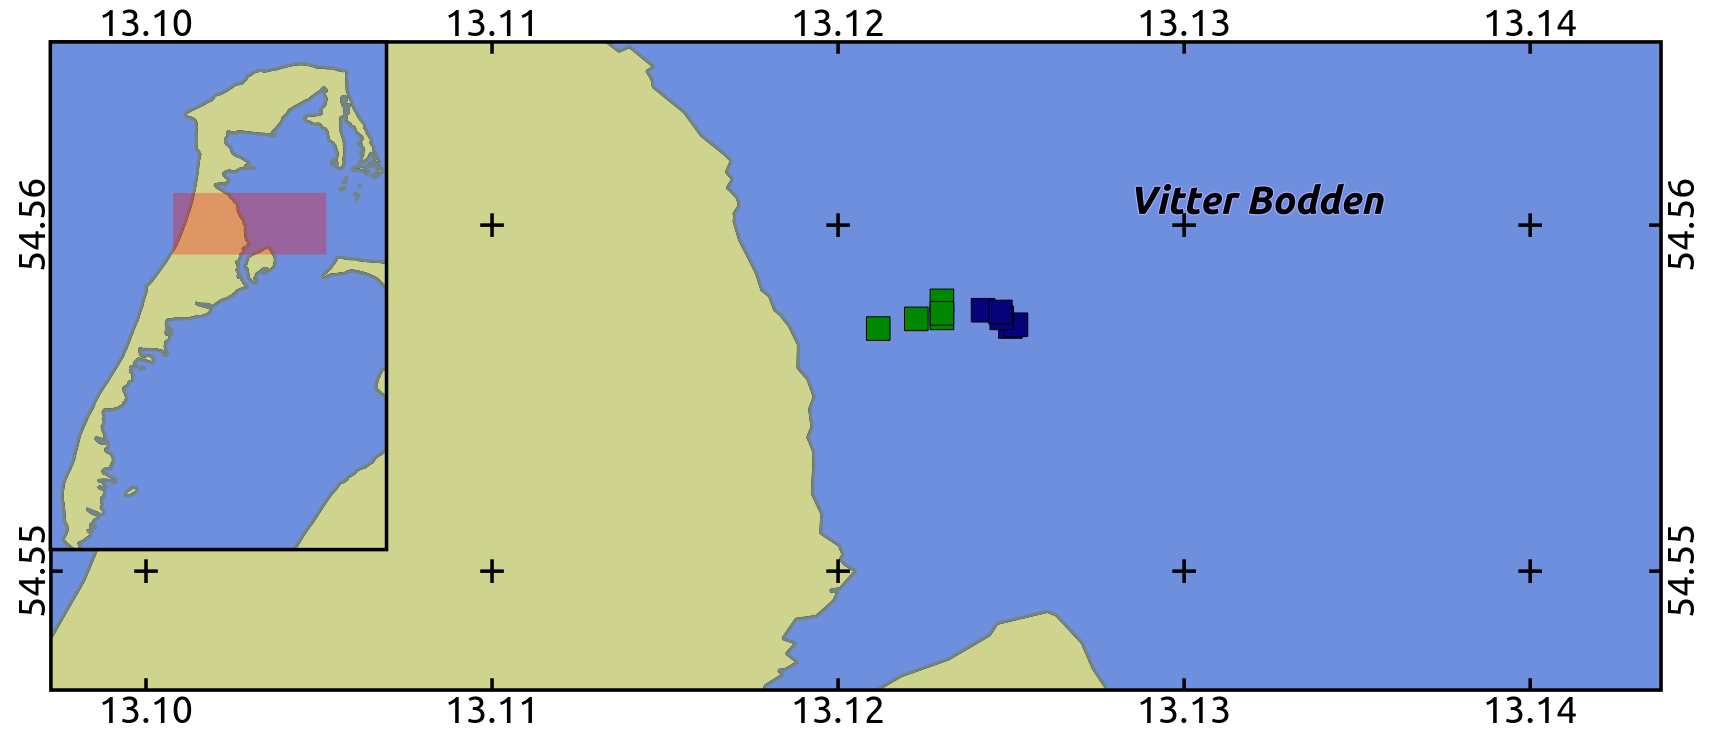
\includegraphics[width=1\textwidth]{images/Vitte.png}
\caption[Probenahmepunkte Vitte]{Probenahmepunkte Vitte; Markierungen: grün = dichte Vegetation, blau = spärliche Vegetation; Maßstab: 1:160.000}
\label{Vitte}
\end{figure}


Die Probennahmestandorte lagen im Flachwasserbereich südlich des Vitter Hafens und nördlich der Fährinsel. Hier ist das Befahren mit motorbetriebenen Wasserfahrzeugen laut Nationalparkverordnung verboten \citep{landesamt_fur_forsten_2002}.

Der makrophytendominierte Standort mit einer mittleren Wassertiefe von \unit{0,83}{\metre} zeigt eine dichte Bedeckung der lose auf dem Boden aufliegenden Braunalge F. vesiculosus f. filiformis. Darin zahreich eingestreut sind winterannuelle Myriophylliden und Parvopotamiden. Der Makrophytenarme Standort hingegen ist auf einer kleinen Sandbank mit einer mittleren Wassertiefe von \unit{0,62}{\metre} gelegen. Hier wachsen vereinzelt Parvopotamiden und die erst später im Jahr aus den Oosporen auskeimenden Chariden. 


\subsubsection{Griebener Bucht (Milena Kafka, verändert)}

Die Griebener Bucht ist Teil des Vitter Boddens und liegt im Nordosten der Insel Hiddensee. Sie ist nur im Süden zum Vitter Bodden hin geöffnet, ansonsten umschlossen von Land. Im Westen liegt der Ort Grieben und im Osten die Bessinsche Schaar \citep{mobus_2000}. Durch die vorwiegenden Westwinde wird  Geschiebemergel aus dem Pleistozän vom Nordufer der Insel abradiert und in südöstliche Richtung durch Hakenbildungen (Alt- und Neu-Bessin) abgelagert \citep{naumann_2012}.

Der Alt-Bessin begann vor 300 bis 500 Jahren zu wachsen, während sich der vorgelagerte Neu-Bessin erst seit etwa 100 Jahren bildet und jährlich \unit{30 bis 60}{\metre} wächst \citep{karge_2007}. Nach \cite{mobus_2000} würden der Bug und der Altbessin zusammenwachsen, wenn für die Schiffahrt zwischen Hiddensee und Rügen die Libben-Fährrinne nicht ausgebaggert werden würde.

Die Griebener Bucht ist im Mittel etwa \unit{1}{\metre} tief \citep{flugge_2004, hendreschke_2009} und als Schutzgebietszone I des Nationalparks ausgewiesen, die das Befahren mit Wasserfahrzeugen, Angeln und Baden untersagt. Ihre Salinität beträgt 8,11 – 8,66 PSU (eigene Messungen von Juli bis September) und gehört nach \cite{gosselck_2011} ebenso wie der Vitter Bodden zur $\beta$ – mesohalinen Zone.

\begin{figure}[htb]
\centering
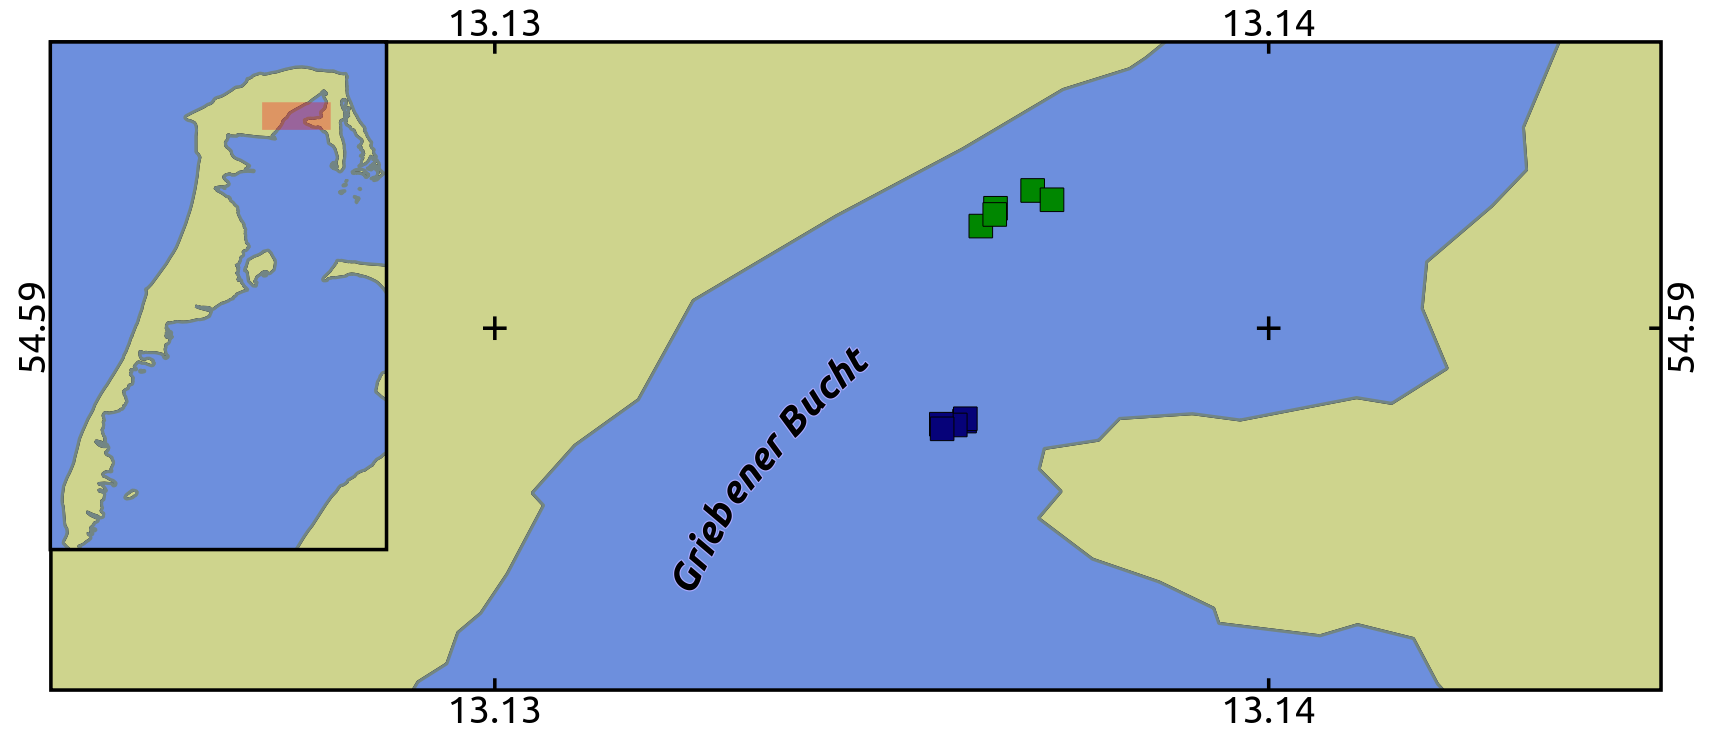
\includegraphics[width=1\textwidth]{images/Grieben.png}
\caption[Probenahmepunkte Griebener Bucht]{Probenahmepunkte Griebener Bucht bei Hiddensee; Markierungen: grün = dichte Vegetation, blau = spärliche Vegetation; Maßstab: 1:6700}
\label{Grieben}
\end{figure}


Der makrophytendominierte Standort für die Probenahmen befand sich \unit{80}{\metre} vom Ufer entfernt am Nordende des Ortes Grieben und die mittlere Wassertiefe dort beträgt \unit{0,87}{\metre}. Hier zeigt sich ein Mosaik aus Parvopotamiden, insbesondere mit Ruppia cirrhosa als rasenhaft bestandsbildende Art, aus Chacareen und Fucus vesiculosus f. filiformis. Der makrophytenarme Standort befand sich mit einer mittleren Tiefe von \unit{0,65}{\metre} \unit{300}{\metre} südöstlich nahe der Ausbuchtung des Alten Bessins. Hier fanden sich vereinzelt Characeen, Parvopotamiden und lose Bällchen des baltischen Blasentangs.



\subsection{Weitere Buchten und Bodden entlang des Salzgradienten}


Es wurden in zwei Bundesländern insgesamt fünf Standorte von West nach Ost ausgewählt: die Geltinger Bucht in der Flensburger Förde, die Orther Bucht südlich der Insel Fehmarn, das Salzhaff in der Wismarer Bucht, der Vitter Bodden bei Hiddensee und die Spandowerhagener Wiek bei Usedom.


\begin{figure}[htb]
\centering
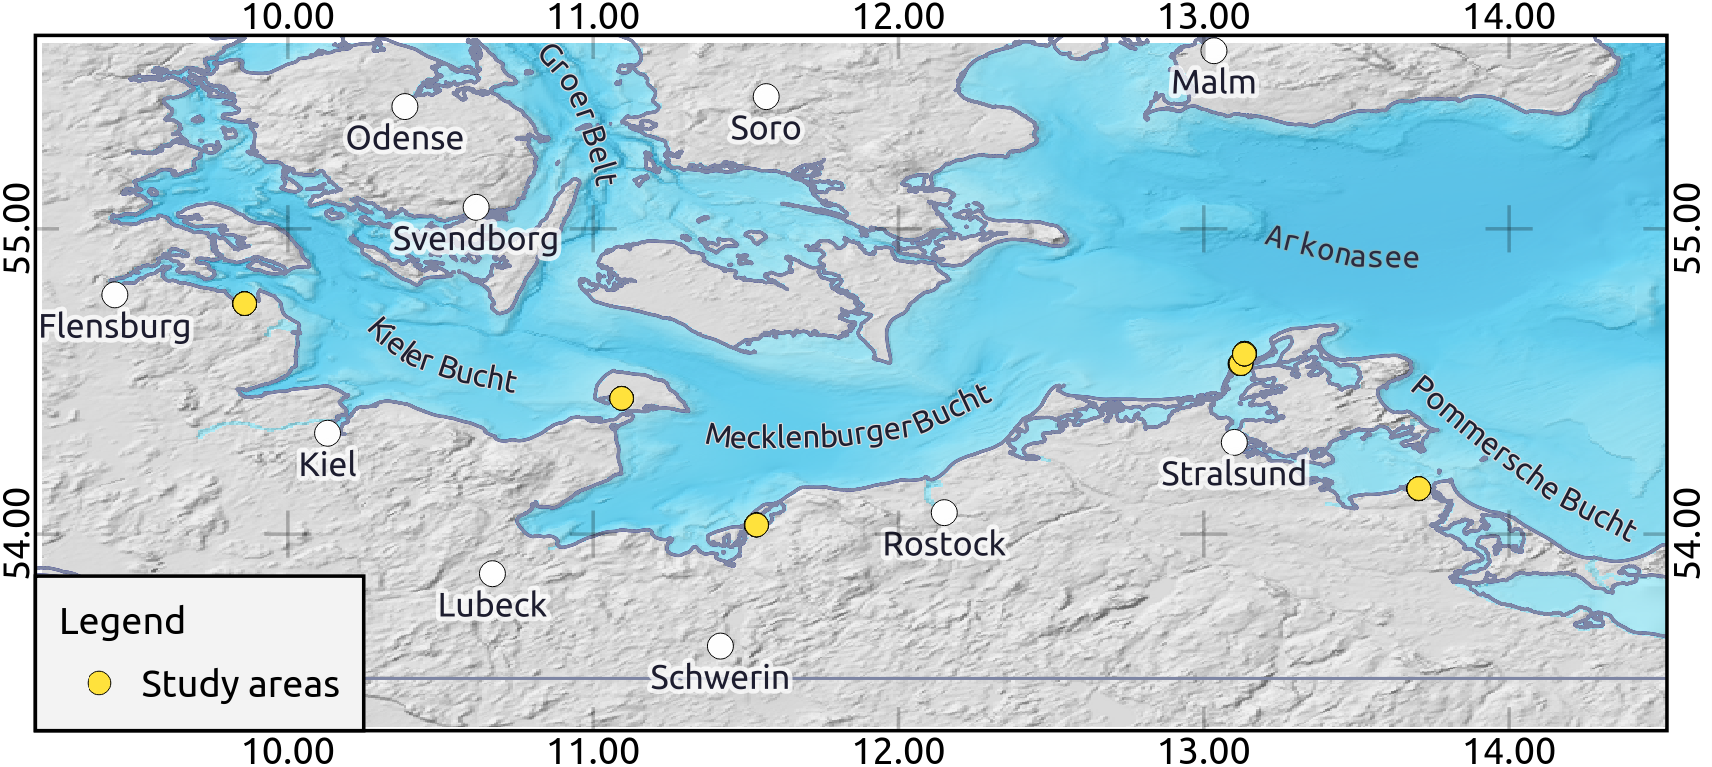
\includegraphics[width=1\textwidth]{images/Uebersicht.png}
\caption[Übersichtskarte der Probenahmestandorte entlang des Salzgradienten]{Probenahmestandorte entlang des Salzgradienten, von links nach rechts: Geltinger Bucht, Orther Bucht, Salzhaff, Hiddensee (Vitter Bodden und Griebener Bucht), Spandowerhagener Wiek; Maßstab: 1:1700000}
\label{Uebersicht}
\end{figure}




\subsubsection{Geltinger Bucht (Antje Kerkow)}


\begin{figure}[htb]
\centering
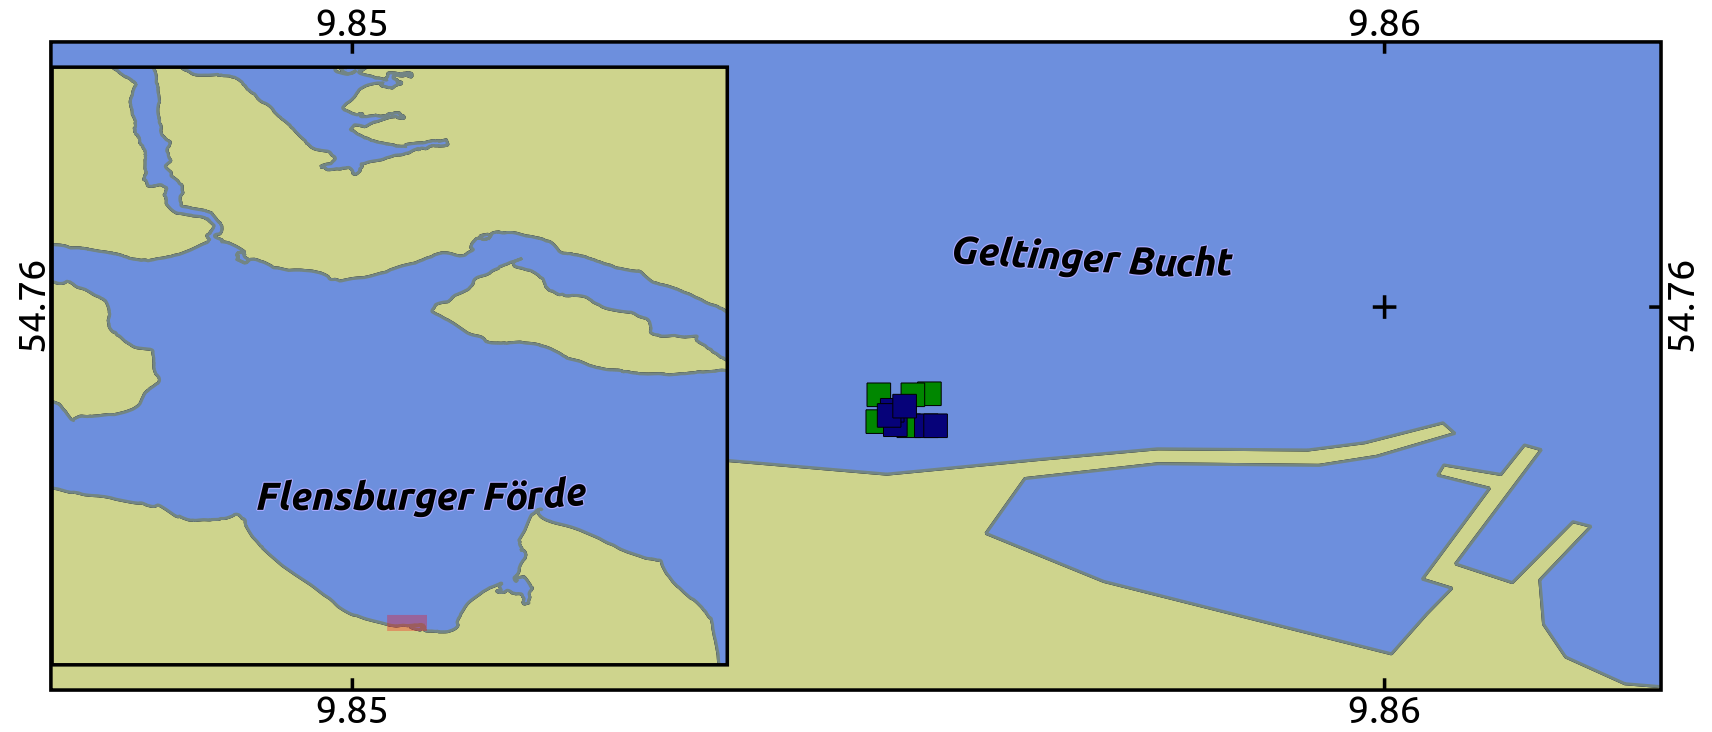
\includegraphics[width=1\textwidth]{images/GB.png}
\caption[Probenahmepunkte Geltinger Bucht]{Probenahmepunkte Geltinger Bucht; Markierungen: grün = dichte Vegetation, blau = spärliche Vegetation; Maßstab: 1:5000}
\label{GB}
\end{figure}


Die Geltinger Bucht ist ein südlicher Ausläufer der Flensburger Außenförde mit einer West-Ost-Ausdehnung von \unit{7,3}{\kilo\metre} und einer Nord-Süd-Ausdehnung von \unit{5}{\kilo\metre}. In ihrem Außenbereich ist sie \unit{20}{\metre} tief \citep{nikulina_2009}, jedoch verfügt sie auch über Steinriffe und ausgedehnte Flachwasserzonen mit Seegrasbeständen \citep{landesbetriebfurkustenschutznationalparkundmeeresschutzschleswig-holstein_2013}.

Die Bucht entstand durch den Rückzug des Gletschereises der Weichseleiszeit. Durch Randmöranen entstanden Höhenzüge, die die Bucht in NNW und SSE-Richtung keilförmig einschlossen. Das Grundmoränenbecken dazwischen wurde während des Meeresspiegelanstieges der Litorinatransgression mit Wasser gefüllt \citep{reisch_1997}.

Der Salzgehalt der Geltinger Bucht wird beeinträchtigt durch Stürme, die salziges Ostseewasser über die Holnisschwelle drücken und damit das Tiefenwasser erneuern \citep{nikulina_2009}. Der Süßwassereinstrom  in die Flensburger Förde ist mit \unit{\430}{\kilo\cubic\metre}/Jahr \citep{lanu_2001} dagegen gering.
Das Wasser im tiefen Zentral- und Außenbereich der Bucht ist saisonal geschichtet und wird als meso-polyhalin eingestuft \citep{reimers_2005}. \cite{kandler_1963,exon_1972} und \cite{bluhm_1990} maßen Salzgehaltswerte zwischen 20 und 26 PSU für das Wasser am Grund und 15 bis 20 PSU für das Oberflächenwasser. Die küstennahen Bereiche hingegen werden als mesohalines äußeres Küstengewässer eingestuft. Zum Zeitpunkt der eigenen Untersuchung betrug der Salzgehalt dort zwischen 9,8 und 10,1 PSU.

Der Vegetationsbewuchs der Bucht ist geprägt durch ein dichtes Vorkommen der Arten Fucus vesiculosus und Ruppia cirrhosa . Zwischen 1900 und 1950 wurde ebenfalls das Vorkommen von Chara aspera, Chara baltica, Lamprothamium papulosum, Zannichellia palustris, Chorda filum und Fucus serratus dokumentiert \citep{mertens_2007}.


\subsubsection{Orther Bucht (Antje Kerkow)}

\begin{figure}[htb]
\centering
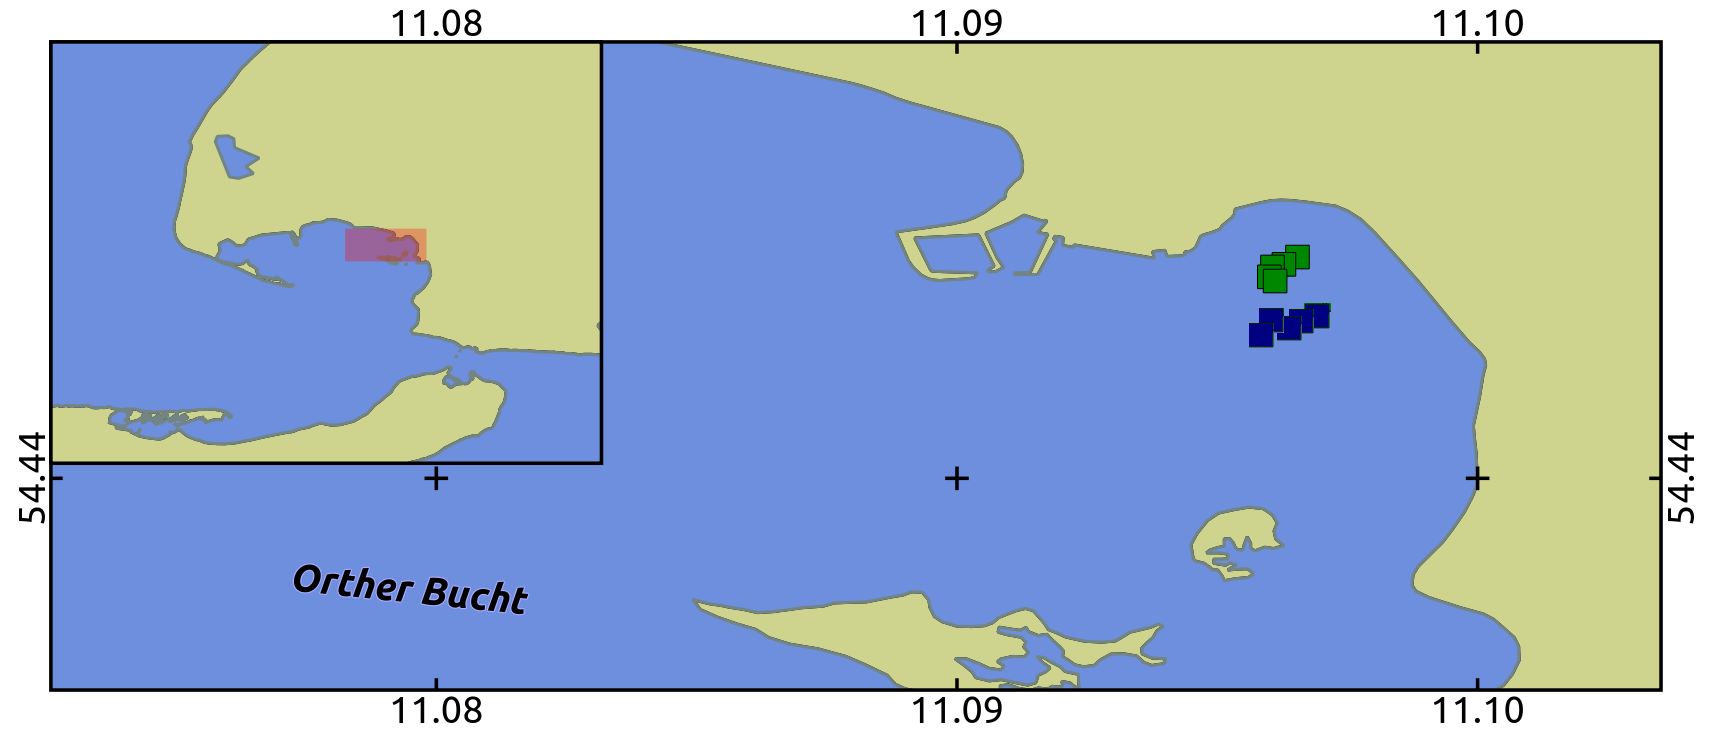
\includegraphics[width=1\textwidth]{images/OB.png}
\caption[Probenahmepunkte Orther Bucht]{Probenahmepunkte Orther Bucht; Markierungen: grün = dichte Vegetation, blau = spärliche Vegetation; Maßstab: 1:10000}
\label{OB}
\end{figure}



Die Orther Bucht liegt mit einer maximalen Tiefe von \unit{4,1}{\metre} \citep{seekartefehmarnsundkartograph_unbekannt_1902} an der Südwest- Seite der Insel Fehmarn. Die Landschaft in dieser Region ist ein Jungmoränengebiet des Schleswig-Holsteinischen Hügellandes, das von der Weichseleiszeit geformt wurde. Die Bucht misst \unit{4,8}{\kilo\metre} in ihrer West-Ost- und \unit{2,8}{\kilo\metre} in ihrer Nord-Süd-Ausdehnung und wird halb umschlossen von der Nehrungshalbinsel Krummersteert. Diese entstand durch die Abtragung von Sand und Geschiebemergel an der Nordwest-Seite der Insel, wo durch die kräftige Brandung das Material gelockert und mit der Strömung in südliche Richtung abtranspoertiert wird \citep{eschwe_2005}.

Die Orther Bucht wird eingestuft als mesohalines inneres Küstengewässer \citep{reimers_2005} und zeigte zum Zeitpunkt der Untersuchung einen Salzgehalt zwischen 11,0 und 11,5 PSU auf.
Die Vegetation ist sehr artenreich, so bilden wurzelnde Arten, insbesondere Characeen, dichte Bestände bis \unit{1}{\metre} Wassertiefe, während in \unit{2 bis 3}{\metre} Tiefe Zostera marina die bestandsbildende Art ist. In einer umfangreichen Vegetationskartierung 2004 wurden folgende Arten gefunden: Tolypellia nidifica, Chara aspera, Chara baltica, Chara canescens, Lamprothamnium papulosum, Ruppia maritima, Zostera marina, Zannichellia palustris, Potamogeton pectinatus, Chorda filum und Fucus vesiculosus. Zudem wurden 1951 auch die Arten Ruppia cirrhosa und Fucus serratus vorgefunden \citep{mertens_2007}.



\subsubsection{Salzhaff (Caroline Lindner, verändert)}

Das Salzhaff liegt im Nordwesten des Bundeslandes Mecklenburg-Vorpommern im Bereich der Koordinaten 54\textdegree\ 2\textquotesingle\ 22\dq\ N bis 54\textdegree\ 5\textquotesingle\ 37\dq\ N und 11\textdegree\ 31\textquotesingle\ 26\dq\ E bis 11\textdegree\ 37\textquotesingle\ 1\dq\ E \citep{nathansen_2014}, nordöstlich der Stadt Wismar und per Luftlinie etwa \unit{35}{\kilo\metre} von Rostock entfernt. Es bildet den Nordostteil der Wismar-Bucht, die zur Mecklenburger Bucht gehört und ist Teil der großräumigen Einheit Beltsee \cite{biele_1997}.

Das Salzhaff wird im Nordwesten durch die Halbinsel Wustrow und die Insel Kieler Ort und im Südwesten durch die Halbinsel Boiensdorfer Werder von der Wismarer Bucht getrennt. Im Süden des Salzhaffs liegt das mecklenburgische Festland.

Die \unit{1,5}{\kilo\metre} breite und \unit{4}{\metre} tiefe Kielung zwischen Kieler Ort und Boiensdorfer Werder verbindet das Salzhaff mit der Wismarer Bucht. Seit 1987 gibt es an der schmalsten Stelle des Kieler Ortes infolge eines sturmbedingten Durchbruchs, der den Haken Kieler Ort von Wustrow trennte, eine zweite Verbindung zur Wismar-Bucht \citep{kohn_1991}.

Das Salzhaff nimmt eine Fläche von \unit{20 bis 22}{\kilo\metre\squared} ein und hat von Südwest nach Nordost eine Länge von \unit{12}{\kilo\metre}. Der vorspringende Tessmannsdorfer Haken teilt das Salzhaff in eine äußere Bucht im Südwesten mit einer Tiefe von bis zu \unit{5}{\metre} und in eine innere Bucht im Nordosten, die eine Tiefe von bis zu \unit{3}{\metre} erreicht \citep{weber_1997}. Die tiefste Verbindung der beiden Buchten bildet der Ellbogen, eine Rinne von etwa \unit{30}{\metre} Breite und \unit{2}{\metre} Tiefe \citep{kohn_1991}.
Die mittlere Tiefe des Salzhaffs liegt bei \unit{2,3}{\metre}. Die maximale Tiefe beträgt \unit{10}{\metre} und befindet sich nordöstlich des Boiensdorfer Werders \citep{kohn_1991}.
Der einzige Süßwasserzufluss ist der Hellbach, der in die innere Bucht mündet, jedoch zu keiner nennenswerten Verringerung des Salzgehaltes führt \citep{weber_1997}. 

Die Mecklenburger Bucht und das Salzhaff unterliegen Salzgehaltsschwankungen, da sie über den Fehmarn Belt mit dem Kattegat und Skagerrak verbunden sind. Daher kamen, wie im Jahr 1994, schon Schwankungen von 8 bis 18 PSU vor. In der Regel liegt der Salzgehalt jedoch über 10 PSU \citep{weber_1997}. Im Juni 2013 konnte dies mit eigenen Messungen von 10,7 PSU im äußeren Salzhaff nachwiesen werden. Das Salzhaff liegt demnach im $ \alpha$ -mesohalinen Bereich \citep{gosselck_2011}. 




\begin{figure}[htb]
\centering
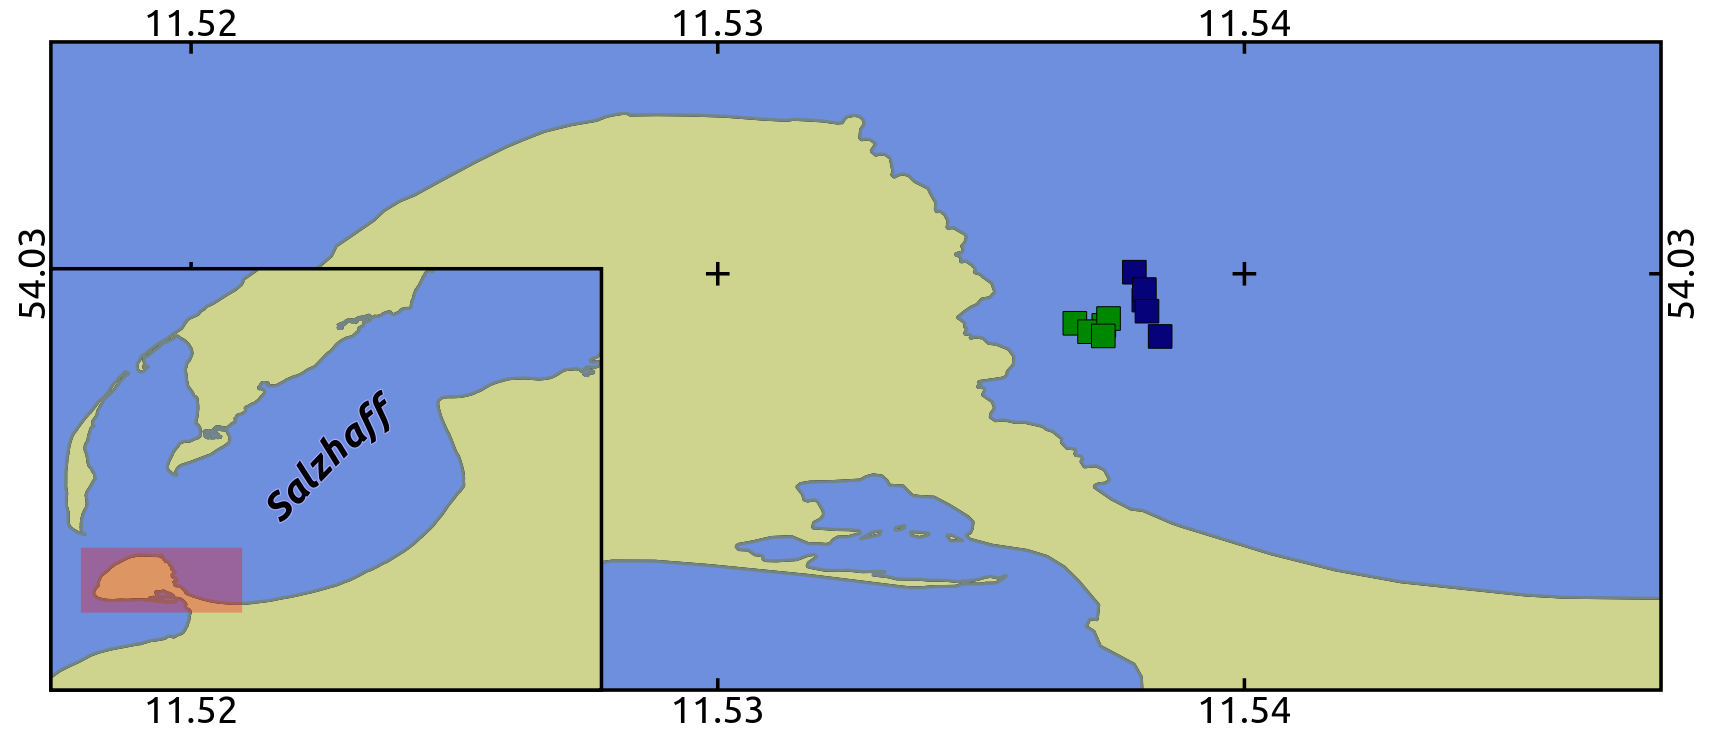
\includegraphics[width=1\textwidth]{images/SH.png}
\caption[Probenahmepunkte Salzhaff]{Probenahmepunkte Salzhaff; Markierungen: grün = dichte Vegetation, blau = spärliche Vegetation; Maßstab: 1:10000}
\label{SH}
\end{figure}



\subsubsection{Spandowerhagener Wiek (Caroline Lindner, verändert)}

Die Spandowerhagener Wiek liegt im Nordwesten der Insel Usedom im Bundesland Mecklenburg-Vorpommern, etwa \unit{22}{\kilo\metre} (Luftlinie) von der Stadt Greifswald entfernt, zwischen den Koordinaten 54\textdegree\ 8\textquotesingle\ 58\dq\ N bis 54\textdegree\ 9\textquotesingle\ 40\dq\ N und 13\textdegree\ 41\textquotesingle\ 55\dq\ E bis 13\textdegree\ 45\textquotesingle\ 6\dq\ E \citep{nathansen_2014}. 
Es handelt sich um eine Bucht, die die Mündung des nördlichen Peenestroms mit dem Greifswalder Bodden verbindet. Sie wird im Osten von der Insel Usedom und im Westen vom vorpommerschen Festland sowie der Insel Struck begrenzt. 

Die Wiek gehört zum Naturschutzgebiet „Peenemünder Haken, Struck und Ruden“ \citep{niedermeyer_2011}.
Das Becken ist flach und wird sowohl von der ausgesüßten Zufuhr der Peene als auch von salzhaltigem Wasser des Greifswalder Boddens gespeist. Es nimmt eine Fläche von \unit{5,4}{\kilo\metre\squared} ein \citep{niedermeyer_2011} und erreicht von Nordwest nach Südost eine maximale Länge von \unit{4}{\kilo\metre}.

Der Greifswalder Bodden ist mit seinen durchschnittlich \unit{5,8}{\metre} etwas tiefer als die flache Spandowerhagener Wiek \citep{meyer_1998}, deren Tiefe bei Struck \unit{2,2}{\metre} beträgt \citep{bartels_1998} und gegenüber im Süden der Wiek bei Freest eine mittlere Tiefe von \unit{1,2}{\metre} aufweist (Buckmann et al 1998). Der Flachwasserbereich ist durch die Fahrrinne der Peene und der etwa \unit{4}{\metre} tiefen Rinne zum Kühlwasserkanal des ehemaligen Kerkraftwerks Nord durchzogen \citep{gosselck_2007}.

Je nach Wasserstand kommt es im Bereich der Peenemündung und des Peenestroms zu salzhaltigem Einstrom aus dem Greifswalder Bodden oder zum Ausstrom von Wasser geringer Salinität aus der Peene \citep{buckmann_1998}. Dadurch kann der Salzgehalt im nördlichen Peenestrom und damit in der Spandowerhagener Wiek zwischen 1 und 8,5 PSU erheblich schwanken \citep{meyer_1998}.

Im Bereich der Spandowerhagener Wiek bei dem Ort Freest wurde eine sprunghafte Abnahme des Salzgehaltes von etwa 6 bis 9 PSU im Greifswalder Bodden auf 3 PSU im Mündungsgebiet festgestellt \citep{gunther_1998}. Untersuchungen im Rahmen des BACOSA-Projektes im Juli 2013 am Westufer nahe Spandowerhagen ergaben einen Salzgehalt von 2,7 PSU. Damit liegt die Spandowerhagener Wiek im $\alpha$ - oligohalinen Bereich.



\begin{figure}[htb]
\centering
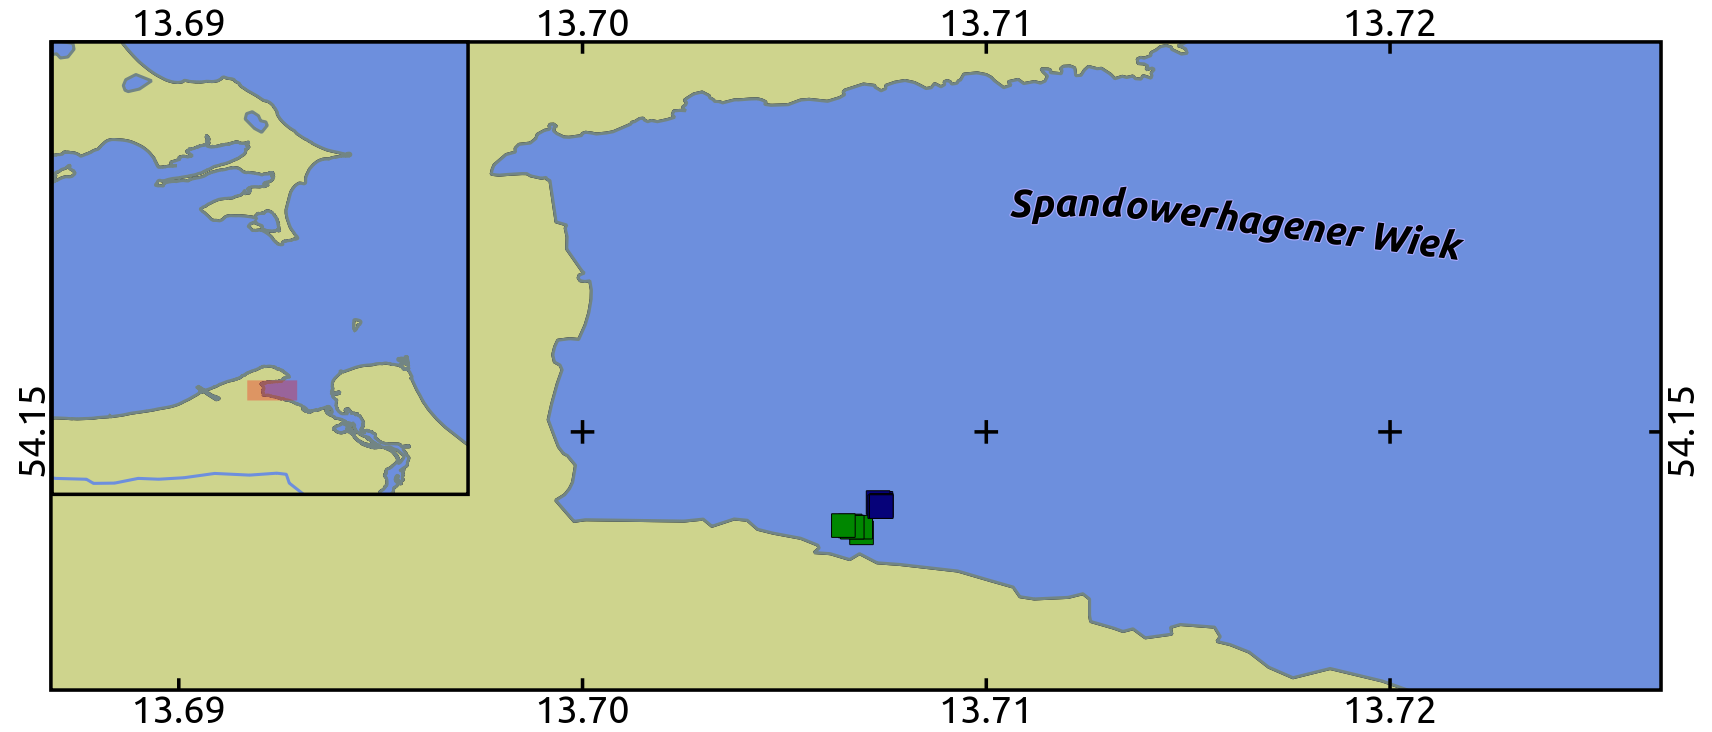
\includegraphics[width=1\textwidth]{images/SW.png}
\caption[Probenahmepunkte Spandowerhagener Wiek]{Probenahmepunkte Spandowerhagener Wiek; Markierungen: grün = dichte Vegetation, größere vegetationsfreie Flächen sind nicht vorhanden; Maßstab: 1:13000}
\label{SW}
\end{figure}





\clearpage

\section{Methoden}
\subsection{Probenahmen}

Im Hauptuntersuchungsgebiet, in den Boddengewässern östlich Hiddensees gelegen, erfolgte eine umfassende Studie der Zusammenhänge vieler Einzelparameter bei denen der Einfluss der Zeit jeweils mitberücksichtigt wurde. Hier wurden jeweils an zwei Standorten fünf mal der Wuchs der Vegetation im Verlauf der Wachstumssaison von Juni bis September untersucht, davon zwei mal zusätzlich die Biomasse. Das Sediment wurde drei mal im Verlaufe der Saison untersucht. Parallel erfolgten Studien zu Strömungsverhältnissen, gelöstem Sediment in der Wassersäule und zu Phyto- und Zooplankton, ebenfalls fünf mal im Jahr an den gleichen Standorten.

Die Studie erfolgte in Gemeinschaftsarbeit von fünf Wissenschaftlerinnen, dabei wurden die Probenahmetermine für verschiedene Untersuchungen möglichst zeitnah miteinander verbunden, sodass bei der Auswertung des Datenmaterials aufeinander Bezug genommen werden konnte(Die genauen Termine sind in Tabelle            \ref{Probenahmetermine} notiert.). Für die Befahrung und Beprobung der Standorte innerhalb des Nationalparkes lag eine Genehmigung der Aufsichtsbehörde des zuständigen Nationalparkamtes vor.

Zusätzlich zu den Hiddenseer Bodden wurden einmalig im Juni und Juli an 4 Standorten entlang des Salzgradienten in flachen Buchten und Boddengewässern der Ostsee  in Zusammenarbeit mit weiteren Wissenschaftlern der Universitäten Rostock und Kiel Vegetation, Sediment, Phytoplankton und suspendiertes Material untersucht(Probenahmetermine siehe Tabelle \ref{Salztabelle}.).

An jedem Standort wurde zwischen 2 Gruppen unterschieden: eine mit dichter Vegetation (über \unit{50}{\%} Deckung) und eine ohne oder nur mit spärlicher Vegetation (nicht mehr als \unit{2}{\%} Deckung zu Beginn der Studie). In jeder Gruppe gab es fünf Messparallelen. Diese waren Plots der Größe zwei mal zwei Meter, die circa acht bis zwölf Meter voneinander entfernt lagen und die jeweils homogen in ihrem Vegetationsbild waren. Um diese Flächen im Jahresverlauf untersuchen zu können, waren sie jeweils an ihrer Südwest-Ecke mit einer nummerierten Schwimmboje markiert.

Es wurde versucht, die Gruppen möglichst nah aneinander und in der gleichen Wassertiefe zu platzieren, jedoch ließ sich dies nur bedingt in der Praxis umsetzen. Damit sich die Vegetation zwischen den Gruppen deutlich unterschied, mussten sie \unit{30-300}{\metre} voneinander entfernt liegen, was zum Beispiel in der \unit{54}{\metre} schmalen Griebener Bucht bedeutet, dass sich die Gruppen auf unterschiedlichen Seiten der Bucht befanden. 


\begin{table}[htb]
\caption{Übersicht Untersuchungen und Probenahmetermine}
\begin{tabular}{lllll}
\toprule
Nr. &  Date & Vitte & Date & Grieben\\
\midrule
\multirow{3}{*}{1} & Jun 04 & Vegetation & Jun 09 & Vegetation \\
 & Jun 05 & Susp. Material, Plankton & Jun 11 & Susp. Material, Plankton \\
 & Jun 05 & Sediment & Jun 11 & Sediment \\
\midrule
\multirow{4}{*}{2} & Jul 03 & Vegetation & Jul 05 & Vegetation \\
 & Jul 03 & Susp. Material, Plankton & Jul 05 & Susp. Material, Plankton \\
 & Jul 06 & Biomass  & Jul 05 & Biomass \\
 & Jul 05 & Sediment (F. Bitschofsky)\\
 \midrule
 \multirow{4}{*}{3} & Aug 01 & Susp. Material, Plankton & Jul 30 & Susp. Material, Plankton\\
 & Aug 01 & Sediment & Jul 30 & Sediment\\
 & Aug 06 & Vegetation & Aug 07 & Vegetation\\
 & Aug 06 & Biomass & Aug 07 & Biomass\\
 \midrule
 \multirow{3}{*}{4} & Aug 19 & Susp. Material, Plankton &  Aug 17 & Susp. Material, Plankton\\
 & Aug 19 & Sediment & Aug 17 & Sediment\\
 & Aug 21 & Vegetation & Aug 21 & Vegetation\\
 \midrule
 \multirow{2}{*}{5} & Sep 16 & Susp. Material, Plankton & Sep 16 & Susp. Material, Plankton\\
 & Sep 22 & Vegetation & Sep 22 & Vegetation
\bottomrule
\end{tabular}
\label{Probenahmetermine}
\end{table}




\subsection{Vegetationskartierung}

Um die Vegetation (und weitere Parameter) zu untersuchen, wurden die Plots mit einem motorisieren Ruderboot von der Lee-Seite angefahren, wobei unmittelbar in der Nähe eines Plots der Motor möglichst nicht in Betrieb genommen wurde. Der Anker wurde so geworfen, dass er weit genug entfernt war, um kein Sediment über der Fläche aufzuwirbeln und dass das Boot an der Lee-Seite der Fläche zum Stehen kam. Dann wurde (nach der Lichtmessung und der Wasserprobeentnahme für weitere Analysen) ein absenkbarer Aluminium-Vegetationsrahmen der Größe zwei mal zwei Meter so abgelegt, dass der Zementstein der Schwimmboje die Süd-West-Ecke des Plots einnahm.

Nun wurde per Schnorcheln die Vegetationsbedeckung insgesamt und für jede vorkommende Pflanzen-und Großalgenart geschätzt. Auch fädige Algen, wurden mit berücksichtigt und Proben davon eingepackt. 

Zur Identifizierung der nicht ohne Hilfsmittel erkennbaren Arten, insbesondere der Characeen-Arten, wurden anfänglich jeweils gleich aussehende Exemplare aus dem Plot-angrenzenden Gebiet entnommen und im Labor mit dem Binokular bestimmt, später im Jahr konnten sie bei guten Sichtverhältnissen ohne Hilfsmittel bestimmt werden. Die fädigen Algen wurden nur bestimmt, sofern sie als Bestand aus nur einer Art bestanden, jedoch nicht, wenn es sich um ein Geflecht unterschiedlicher Arten handelte.

Die Gefäßpflanzen wurden bestimmt nach \cite{van_de_weyer_2007} und \cite{rothmaler_2005} und die Algen nach \cite{pankow_1971}.


\begin{table}[h]
\centering
\caption{Skala für die Schätzung der Makrophytenbedeckung}
\begin{tabular}{llr}
\toprule
Code	&& Translation\\
\midrule
0,5	 	&& \unit{<1}{\%} \\
2 		&& \unit{1-4}{\%} \\
5 		&& \unit{5}{\%}\\
\midrule
10 		&& \unit{6-14}{\%}\\
20 		&& \unit{15-24}{\%}\\
30 		&& \unit{25-34}{\%}\\
40		&& \unit{35-44}{\%}\\
50		&& \unit{45-54}{\%}\\
\midrule
60		&& \unit{55-64}{\%}\\
70		&& \unit{65-74}{\%}\\
80		&& \unit{75-84}{\%}\\
90		&& \unit{85-94}{\%}\\
100		&& \unit{95-100}{\%}\\
\bottomrule
\end{tabular}
\label{Deckung}
\end{table}



Die Schätzung der Deckungsgrade erfolgte nach einer Skala, die im Bereich der unteren Deckungsgrade an die Braun-Blanquet-Skala angepasst, jedoch im Bereich größerer Deckungen eine höhere Genauigkeit aufweist (Vgl. Tabelle \ref{Deckung}).

Außerdem wurde eine Höhenstufenkartierung an jedem Plot durchgeführt. Hierbei wurde die Deckung der Vegetation insgesamt und für jede vorkommende Art in unterschiedlichen Abständen vom Grund geschätzt. Dabei wurden auf den Wuchshöhen \unit{5}{\centi\metre}; \unit{10}{\centi\metre} und alle weiteren zehn Zentimeter bis zur Oberfläche kartiert. Zur Orientierung dabei wurden zwei Stäbe gesetzt, die bis zur Null-Marke an zwei Plot-Enden ins Sediment gesteckt wurden und an denen Ösen für jede Wuchshöhe angebracht waren, in die eine Schnur eingespannt werden konnte. Die Deckungen wurden dann auf einem Unterwasserprotokoll notiert.






\subsection{PV und PVI}

Der Anteil des Pflanzenvolumens am Gesamtwasservolumen (Plant Volume Infested, PVI), wird nach \cite{jeppesen_1998, schriver_1995, canfield_1984} berechnet als 

\begin{equation*}
\frac{\text{Mittlere Wuchshöhe} * \text{Deckung}}{\text{Wassertiefe}}.
\end{equation*}

Die mittlere Wuchshöhe, multipliziert mit der Deckung, wird auch als 'Area specific plant volume', PV, bezeichnet \citep{jeppesen_1998}.\\
In dieser Studie wurde ein genaueres Verfahren angewendet, in dem die Deckungen aller Höhenstufen (vgl. Vegetationskartierung, Höhenstufenkartierung) bei der Berechnung berücksichtigt wurden:


\begin{align*}
 PV &=\sum_{i=a}^n \frac{H_i * C_i}{100} & H_i &=\text{Länge einer jeden Höhenschicht}\\ 
 & & C_i &=\text{Deckung auf dieser Höhenschicht}\\
 & & a-n &=\text{Höhenstufen vom Boden}\\
 & &     &\text{\quad bis zur Wasseroberfläche}\\
 PVI &=\frac{PV}{\text{mittlere Wassertiefe}}.\\
\end{align*}



\subsection{Mittlere Wassertiefe}

Die Wassertiefen wurden einmalig an jedem Plot mit dem Zollstock gemessen und zusammen mit der Uhrzeit notiert. Später wurde der aktuelle Pegelstand der nächstgelegenen Pegelmessstation und deren Mittelwasserstand recherchiert. Mit diesen Informationen konnte der mittlere Wasserstand für jeden Plot berechnet werden.

Die Pegelmessstationen für die jeweiligen Standorte waren Kappeln für die Geltinger Bucht, Heiligenhafen für die Orther Bucht, Timmendorf für das Salzhaff, Kloster für die Hiddenseeer Standorte und Stahlbrode für die Spandowerhagener Wiek. Die minutengenauen Wasserstände hielten die Wasser- und Schifffahrtsämter von Stralsund und Lübeck bereit. Die Mittelwasserstände stammen von der Webseite Pegelonline der \cite{wasser-_und_schifffahrtsverwaltung_des_bundes_2013}.



\subsection{Biomasse} 


Um die Biomasse zu untersuchen, wurde ein \unit{20}{\centi\metre} hoher quadratischer Stahlrahmen mit einer Kantenlänge von \unit{50}{\centi\metre} angefertigt. Dieser wurde in ungefähr einem halben Meter Abstand zum Hauptplotuntersuchungs-Plot auf dem Boden abgesetzt und leicht ins Sediment eingedrückt. Bei der Auswahl der benachbarten kleineren Fläche, nachfolgend als Miniplot bezeichnet, wurde darauf geachtet, dass sich das Vegetationsbild  möglichst wenig von dem im Hauptuntersuchungs-Plot unterscheidet.

Die Biomasse wurde schnorchelnd mit einer Harke abgeerntet und in einen Angelkescher gefüllt, wobei der Kescher ständig in einer leicht kreisenden Bewegung unter Wasser gehalten wurde, sodass die Biomasse nicht entweichen konnte. Um sicher zu gehen, dass keine Biomasse übersehen wurde, wurde zum Schluss noch einmal ein paar Minuten abgewartet, bis sich die Trübung durch das aufgewirbelte Sediment gelegt hatte und eventuell noch einmal nachgeerntet. Durch die harkende Methode wurde nicht nur die oberirdische sondern auch die Wurzelbiomasse abgeerntet und ging in die Analyse mit ein.

Für den Transport wurde die Biomasse in Plastiktüten verpackt und im Labor möglichst rasch bearbeitet. Hierfür wurde sie gewaschen und Steine und Muscheln herausgesammelt. Anschließend wurde sie bei \unit{105}{\celsius} so lange getrocknet, bis kein Gewichtsverlust durch weiteres Trocknen mehr beobachtet werden konnte. Anschließend wurden die Proben im Exsikkator abgekühlt und gewogen.

Für die Bestimmung des aschfreien Trockengewichtes wurden jeweils etwa \unit{30}{\gram} Trockenbiomasse aus jeder Probe in  Aluminium-Schalen, die vorher bei \unit{500}{\celsius} erhitzt wurden, im Exsikkator abgekühlt sind und danach gewogen wurden, eingewogen. Proben aus Plots mit einer sehr geringen Menge Biomasse wurden vollständig verascht und bereits vor dem Trocknen in Schalen gefüllt, die auf diese Weise behandelt wurden. Die Subproben wurden dann bei \unit{500}{\celsius} drei Stunden im Ofen verbrannt. Die lineare Anheizzeit betrug 3 Stunden. Dann wurden die Proben wieder im Exsikkator abkühlen lassen und erneut eingewogen. Das prozentuale aschfreie Trockengewicht [AFDW (\%)] wurde dann berechnet als:

\begin{align*}
 AFDW(\%)&=\frac{100(B_d-B_b)}{B_d} & B_b &=\text{Gewicht der Biomasse}\\ 
 & &     &\text{\quad verascht bei 500\celsius}\\
 & & B_d &=\text{Gewicht der Biomasse}\\
 & &     &\text{\quad getrocknet bei 105\celsius}\\
\end{align*}




\subsection{Sediment}
\subsubsection{Analytik in Gelände und Labor}
Die Sedimententnahme unmittelbar neben jedem Plot erfolgte mittels eines Stechzylinders mit einem Innendurchmesser von \unit{10}{\centi\metre}, welcher mit Hilfe eines langen Carbon-Rohres vom Boot aus in das Sediment gestoßen wurde. Mit Hilfe einer am Rohr angebrachten, handgefertigten Schelle wurde der Zylinder am Rohr angebracht. Anschließend wurde er mit einem Stopfen mit Rücklassventil oben verschlossen, circa \unit{10}{\centi\metre} lotrecht ins Sediment geschoben und an die Oberfläche befördert, wobei das Rücklassventil beim Herausnehmen aus dem Wasser geschlossen gehalten und der Sedimentkern zusätzlich von unten mit einem Stopfen gesichert wurde. Auf dem Boot wurde zuerst der obere Stopfen abgenommen und das im Zylinder überstehende Wasser mit einem Schlauch von circa \unit{5}{\milli\metre} Innendurchmesser abgesaugt. Danach wurde der untere Stopfen entfernt und der Zylinder auf einem Ständer mit Gummistempel platziert. Das Sediment wurde mit dem Stempel aus dem Zylinder herausgedrückt und die obersten \unit{2}{\centi\metre} mit einem Spatel abgenommen und zur weiteren Untersuchung im Labor in feste Tüten verpackt.

Im Labor wurde jede Sedimentprobe zu einer Mischprobe verarbeitet, sichtbare Tier- und Pflanzenteile wurden herausgesammelt. Für die Bestimmung des Wassergehaltes wurden Aluminiumschälchen vorbereitet. Für 2 Stunden wurden sie bei \unit{500}{\celsius} in den Ofen und danach in den Exsikkator zum Abkühlen gestellt. Anschließend wurden sie mit einer Feinwaage gewogen und das Gewicht notiert.

Aus den Mischproben wurden mit einer manuell vorn eingekürzten Spritze etwa \unit{10}{\milli\litre} Probenmaterial entnommen und in die Aluminiumschälchen gefüllt. Anschließend wurden die Schalen mit dem Probenmaterial eingewogen. Danach wurde das Sediment 12 Stunden bei \unit{105}{\celsius} getrocknet, im Exikkator abgekühlt und erneut eingewogen. Anhand des Gewichtsunterschiedes der Probe vor und nach dem Trocknen konnte der prozentuale Wassergehalt ermittelt werden.

Um den organischen Gehalt in Form des aschfreien Trockengewichtes zu untersuchen, wurde das getrocknete Sediment aus den \unit{10}{\milli\litre}-Proben 12 Stunden bei \unit{500}{\celsius} in den Ofen gestellt, erneut im Exsikkator abgekühlt und eingewogen. Anschließend wurde der Anteil des Glühverlustes am Trockengewicht berechnet.

Für die Korngrößenanalyse wurden weitere \unit{100}{\gram} des frischen Sedimentes abgewogen und nass gesiebt. Dafür wurde eine Siebkaskade mit mittleren Korngrößendurchlässen von \unit{1000}{\micro\metre}, \unit{500}{\micro\metre}, \unit{250}{\micro\metre}, \unit{125}{\micro\metre} und \unit{63}{\micro\metre} verwendet. Der Anteil einer jeden Kornfraktion wurde in bei \unit{105}{\celsius} getrocknete  und danach eingewogene Aluminiumschälchen gefüllt und ebenso wie die \unit{5}{\milli\litre}-Proben mindestens 24 Stunden bei \unit{105}{\celsius} getrocknet und nach dem Abkühlen gewogen. Durch Aufaddieren aller Gewichte der getrockneten Korngrößen abzüglich des prozentualen Wassergehaltes konnte geschlussfolgert werden, wie groß der Anteil der Sedimentfraktion unter \unit{63}{\micro\metre} Durchmesser war. Mit Hilfe dieser Werte konnten die Gewichte aller gröberen Korngrößenfraktionen anteilig zur Summe der Gewichte aller Korngrößen berechnet werden.

Für die weitere statistische Auswertung wurden alle Korngrößenklassen mit dem negativen Logarithmus zur Basis 2 in $ \Phi $-Werte umgerechnet. 
Zur Beschreibung der Korngrößenverteilungen wurden für jeden Plot an jedem Untersuchungstag Median, Mittelwert, Sortierung und Schiefe ausgerechnet und die Werte der jeweiligen Replikate für jedes Datum gemittelt.

Die Sedimentproben entlang des Salzgradienten wurden von Franziska Bitschofsky (BACOSA-Doktorandin der Universität Rostock) aus den Untersuchungsflächen entnommen und bearbeitet. Dabei wurde jeweils nur ein Sedimentkern pro Standort für die Korngrößenanalyse aus dem dichtbewachsenen und aus dem spärlich bewachsenen Bereich entnommen. Aus jedem Kern wurden im Labor 3 Messparallelen untersucht und Mittelwerte (arithmetisches Mittel) gebildet. Die Nasssiebung, das Trocknen und Verbrennen erfolgten auf die gleiche Art wie bei den Hiddenseer Langzeitstandorten.


 
\subsubsection{Berechnungen der Kennwerte}


\begin{align*}
 AFDW(\%)&=\frac{100(S_d-S_b)}{S_d} & AFDW&=\text{Aschfreies Trockengewicht}\\ 
 & & S_b &=\text{Gewicht des Sedimentes}\\
 & &     &\text{\quad verascht bei 500\celsius}\\
 & & S_d &=\text{Gewicht des Sedimentes}\\
 & &     &\text{\quad getrocknet bei 105\celsius}\\
 L(\%)	 &=\frac{100(S_w-S_d)}{S_w} & L&=\text{Wassergehalt}\\
 & & S_w &=\text{Gewicht des feuchten}\\
 & & 	 &\text{\quad Sedimentes}\\
 \\
 S_{d_i} (\%)&=\frac{100*S_d__i}{\sum_{k=a}^f S_d__k} & i&=\text{Gewicht einer Korngrößen-}\\
 & & &\text{\quad fraktion der Kategorien a-f}\\
 S_{b_i} (\%)&=\frac{100*S_b__i}{\sum_{k=a}^f S_b__k}\\
 \\
 S_{d_{<63}} (\%) &=\frac{M-L(\%)}{100}-\sum_{k=a}^e S_d__k & M&=\text{Gesamteinwaage Feucht-}\\
  & & 	 &\text{\quad probe}\\
 \\
 \Phi &=-log_2 \frac{d}{d_0} & d&=\text{Korndurchmesser}\\
 \\
 \tilde{x} &=\Phi_{50} & \tilde{x}&= \text{Median}\\
 \\
 So &=\frac{\Phi_{84}-\Phi_{16}}{4} + \frac{\Phi_{95}-\Phi_5}{6,6} & So &= \text{Sortierung}\\             
 \\
 Sk &=\frac{\Phi_{16}+\Phi_{84}-2*\Phi_{50}}{2*(\Phi_{95}-\Phi_{5})} + \frac{\Phi_{5}+\Phi_{95}-2*\Phi_{50}}{2*(\Phi_{84}-   \Phi_{16})} & Sk &= \text{Schiefe} 
\end{align*}
\\


\subsection{Datenanalyse und Kartenerstellung}

Dateneingabe und Berechnungen erfolgten in Microsoft Office Excel 2007. Mit Histogrammen wurden die mittleren Korngrößen, Sortierung, Schiefe und organischer Anteil der Sedimente sowie der Gehalt der \Unit{< 63}{$ \mu\metre $}-Fraktion und außerdem Deckungsgrade, PVI-Werte, Biomasse und Gehalt der organischen Substanz der Biomasse der Hiddenseer Standorte auf Normalverteilung und Gleichheit der Varianzen untersucht. Anschließend wurde mit dem Mann-Whitney-Test analysiert, ob sich die Parameter zu jedem Zeitpunkt zwischen den dicht und spärlich bewachsenen Arealen in Grieben sowie in Vitte unterscheiden. Mit dem Kruskal-Wallis-Test wurde untersucht, ob sich die Parameter (außer der Biomasse) im Jahresverlauf unterscheiden. Trat dieses Ergebnis ein, wurde mit multiplen Vergleichen mit dem Dunn's Test untersucht, zwischen welchen Tagen sie sich unterscheiden. Innerhalb des Dunn's Tests wurde der \textit{p}-Wert korrigiert. Bei einem \textit{p}-Wert unter 0.05 wurde ein Ergebnis als signifikant gewertet.

Die Ergebnisse wurden mit Boxplots und Balkendiagrammen visualisiert. Aufgrund der geringen Stichprobengröße und des kategorialen Charakters der Daten für die Deckungsgrade wurden die statistischen Größen mit dem Median und der mittleren Abweichung vom Median (MAD) gezeigt. Histogramme, Boxplots und Balkendiagramme wurden mit IBM SPSS Statistics 20 erstellt. Auch der Mann-Whitney-Test und der Kruskal-Wallis-Test wurden damit berechnet. Für multiple Vergleiche mit dem Dunn's-Test wurde das Programm GraphPad Prism 6 benutzt. 

Die Visualisierung der Regressionsmatritzen und die Bestimmung der besten multiplen Regressionsmodelle mittels Rückwärtsselektion wurden mit Minitab 16 durchgeführt. Der Ausschluss eines Parameters aus dem Modell erfolgte ab einem p-Wert von 0,1. 

Die Erstellung der Karten erfolgte mit QGIS 2.0.1. 



\clearpage

\section{Ergebnisse - Hiddenseer Standorte}
\subsection{Detaillierte Vegetationsstruktur}


\subsubsection{Vitte, dicht bewachsener Standort}

\begin{figure}[!htb]
        \centering
        \begin{subfigure}[htb]{0.45\textwidth}
                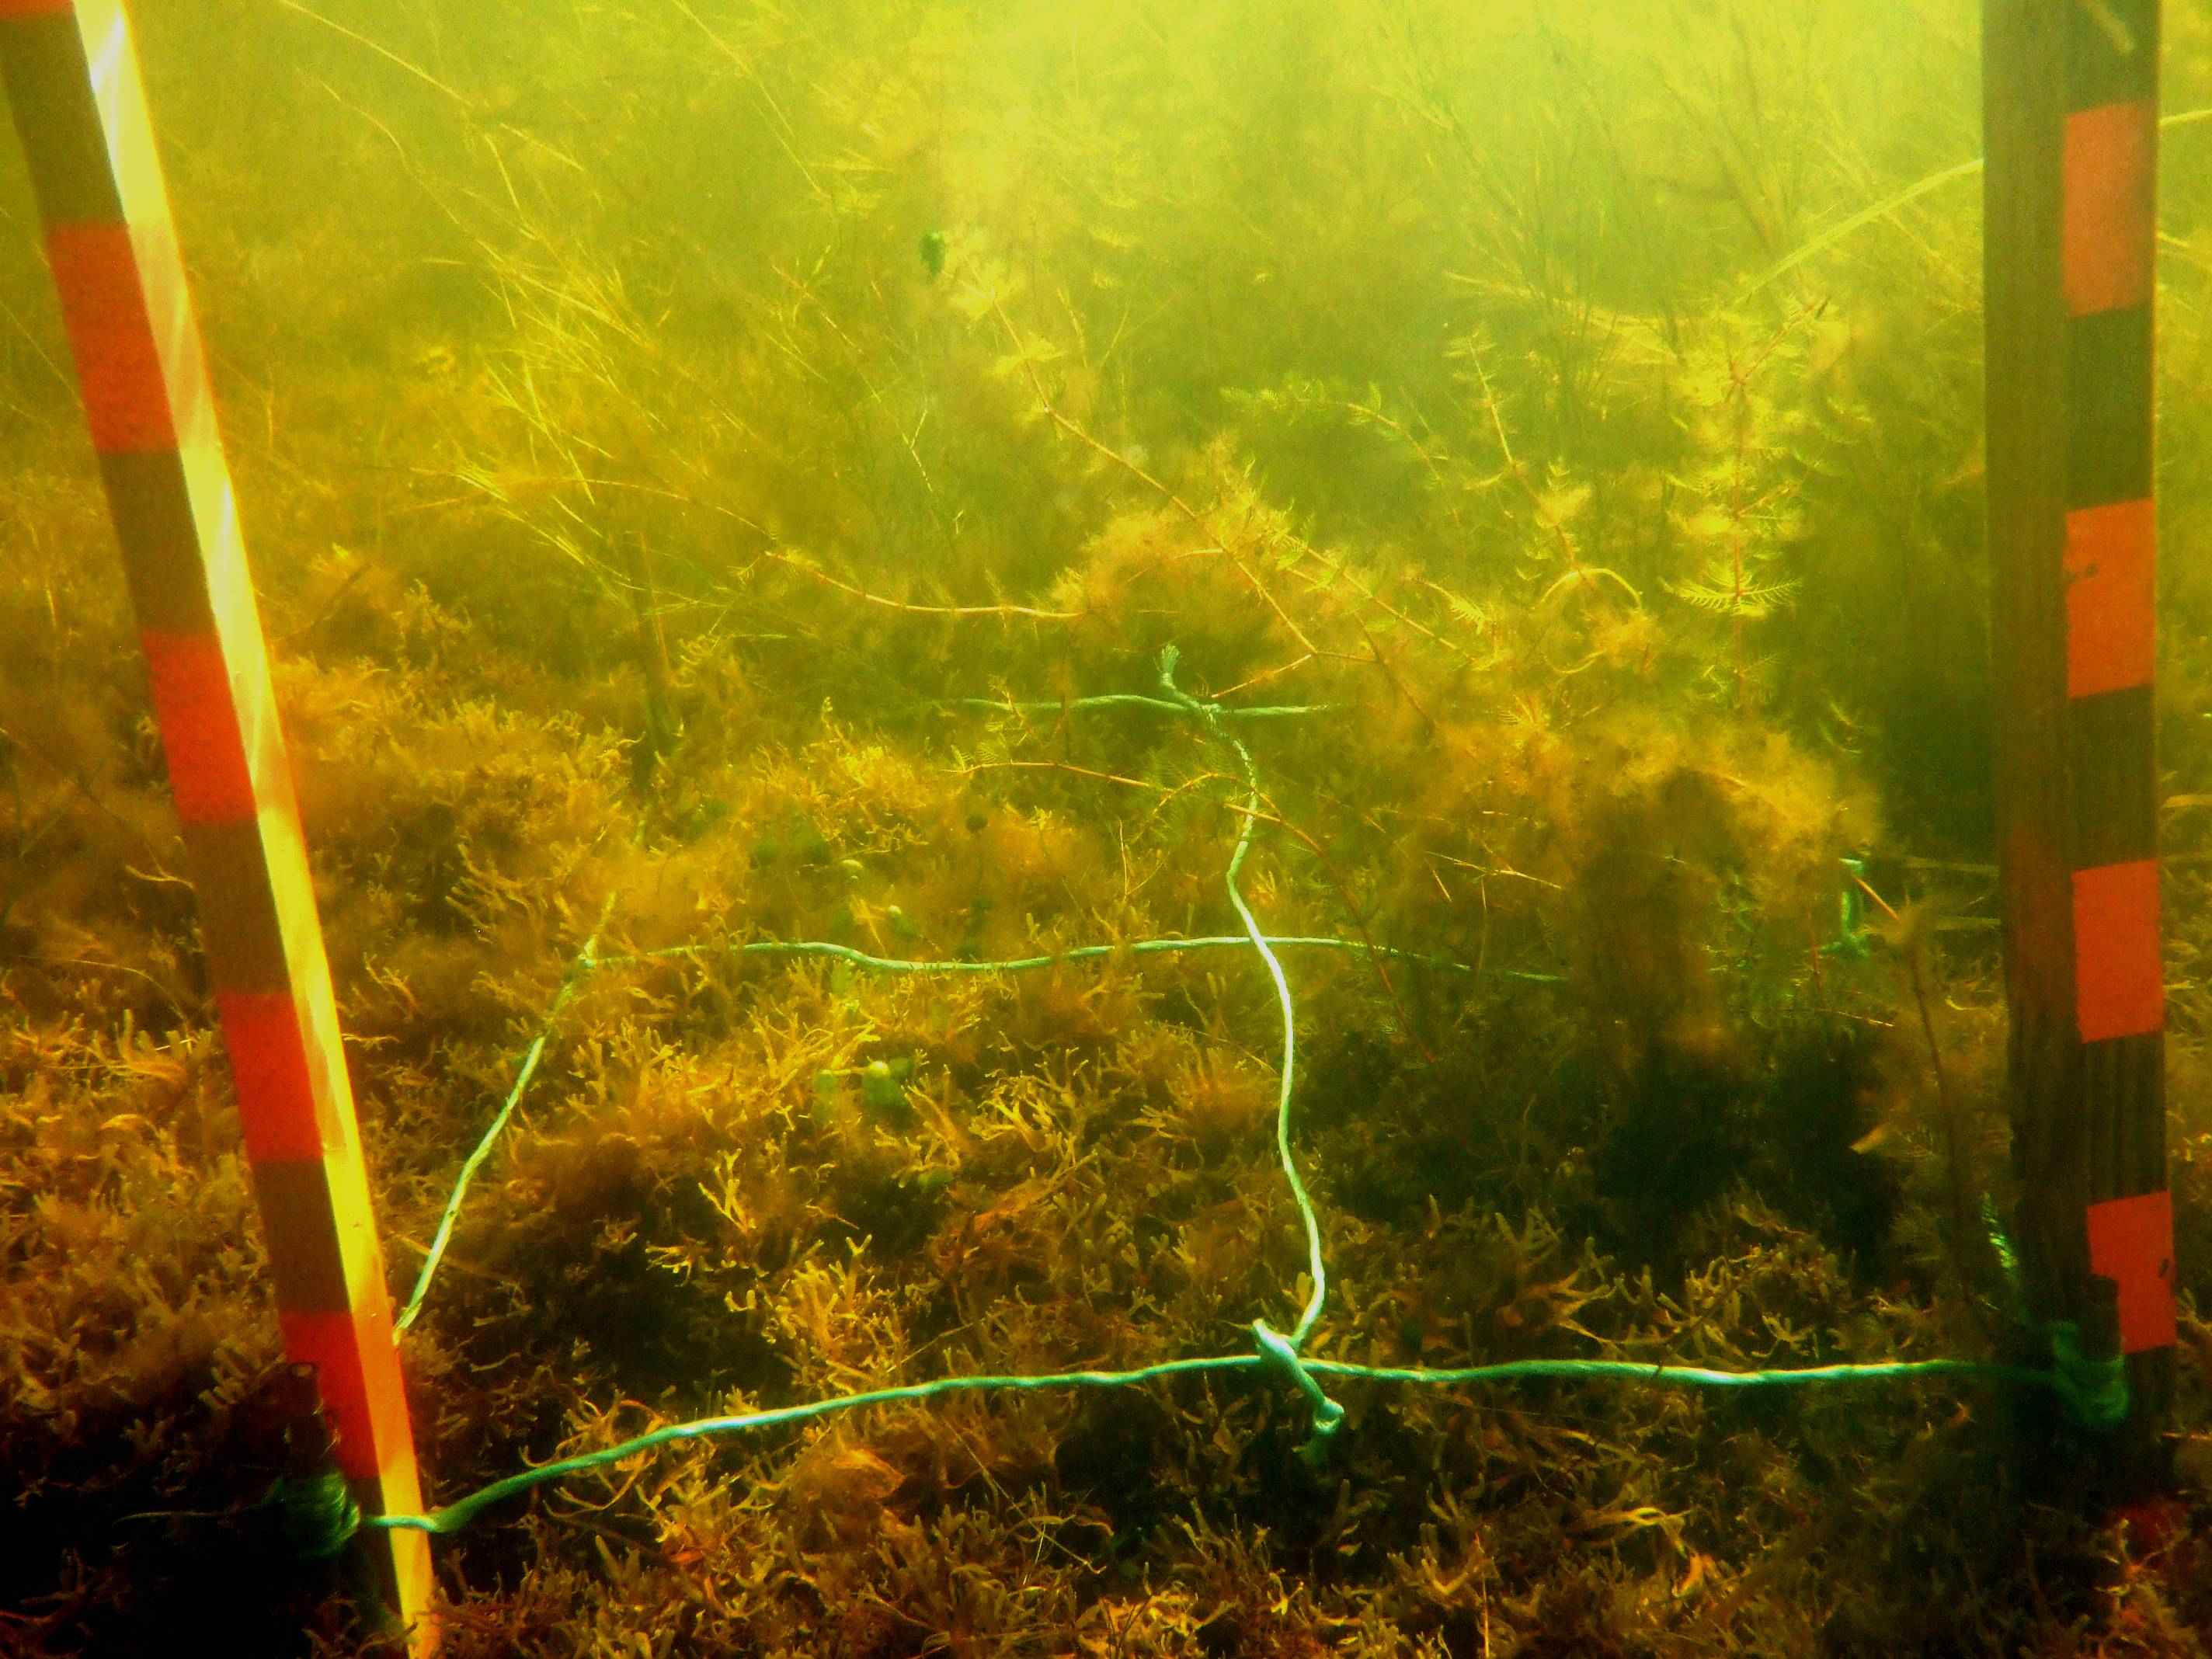
\includegraphics[width=\textwidth]{images/plotpictures/BSP_V+M}
        \end{subfigure}
        \begin{subfigure}[htb]{0.45\textwidth}
                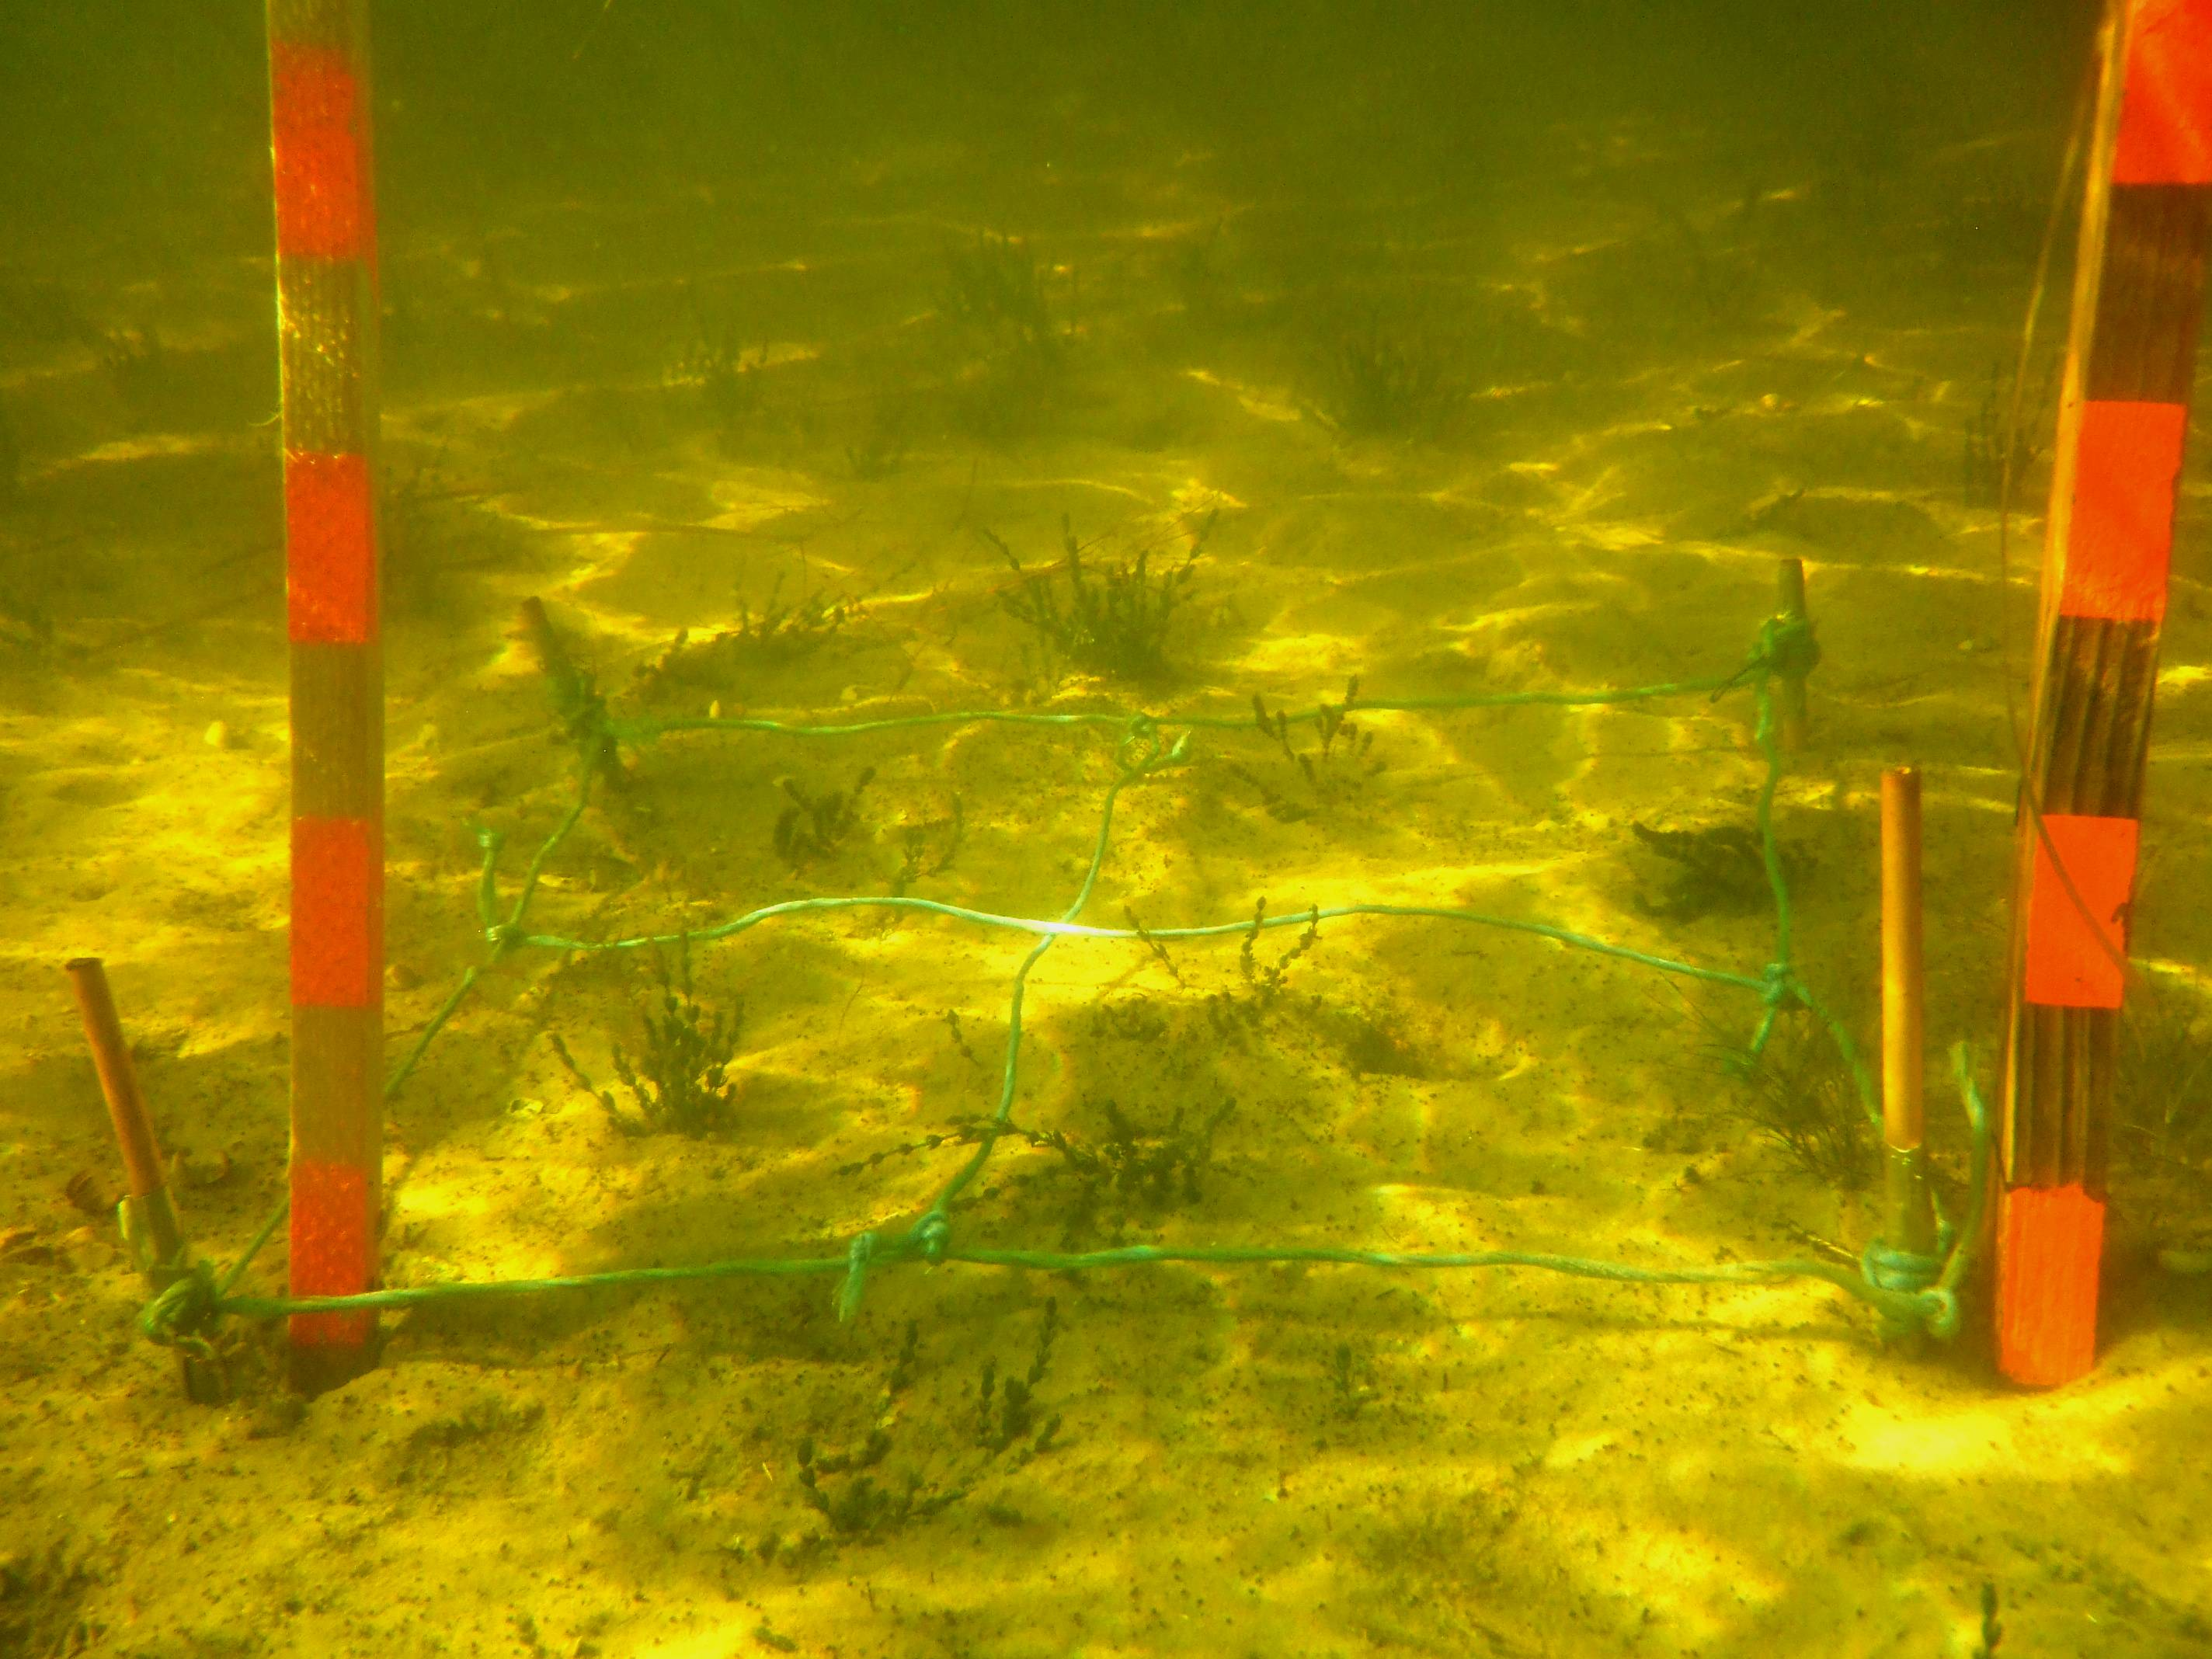
\includegraphics[width=\textwidth]{images/plotpictures/Bsp_V-M}
        \end{subfigure}
        \caption[Fotoaufnahmen der Vegetation in Vitte]{Vegetation in Vitte, vegetationsdominierter Standort 					(links) und  vegetationsarmer Standort (rechts), \unit{0,25}{\metre\squared}- Miniplots, 						Aufnahme August 2013}
        \label{fig:fotos_vitte}
\end{figure}


Die Deckung in Vitte an den vegetationsdominierten Standorten betrug ganzjährig \unit{100}{\%}, wobei der baltische Blasentang \textit{Fucus vesiculosus f. balticus} den Boden vollständig abdeckte. Zwischen dem baltischen Blasentang kam vereinzelt die ebenfalls nicht verwurzelte, kugelförmige Rotalge \textit{Furcellaria fastigiata f. aegagropila} mit einer Deckung von \unit{0,5}{\%} während des gesamten Beobachtungszeitraumes vor. Während die sessilen Makroalgen im Juni bis maximal \unit{5}{\centi\metre}- Wuchshöhe kartiert wurden, sind sie in der Hauptvegetationsperiode (Anfang Juli bis Mitte August) auch auf \unit{10}{\centi\metre} Wuchshöhe mit einer Deckung von \unit{50}{\%} zu finden. Im weiteren Jahresverlauf nimmt die Deckung von \textit{Fucus vesiculosus f. balticus} auf \unit{10}{\centi\metre} Wuchshöhe allmählich wieder ab. Ende August waren es \unit{40}{\%} und Ende September \unit{30}{\%}.

Desweiteren ist die Angiosperme \textit{Potamogeton pectinatus} prägend für den Vitter makrophytendominierten Standort. Mit einer Deckung von \unit{5}{\%} im Mai bis \unit{20}{\%} im August findet sie sich an vielen Stellen zwischen dem dichten Makroalgenteppich und wächst bis an die Wasseroberfläche, an der sich ihr langgestreckter, fadenartiger Wuchs fortsetzt. Insgesamt nimmt die Deckung der Art und die Dichte ihrer Verzweigungen vom Grund zur Oberfläche hin deutlich ab. 

Auch die Angiosperme \textit{Myriophyllum spicatum} findet sich vereinzelt zwischen den Makroalgen mit einer maximalen Deckung von \unit{2}{\%} Ende August. Auch diese zeigt ihre größte Dichte und die meisten Verzweigungen am Grund und nur wenige Äste reichen weiter als \unit{10}{\centi\metre} in den Wasserkörper hinein. Ihre maximale Höhe Ende August beträgt \unit{60}{\centi\metre}.

Im Mai und Juni war der Standort dicht bedeckt von Matten filamentöser Algen, die sich freischwimmend dicht am Grund zwischen den aufwachsenden Angiospermen befanden und später im Jahr verschwanden. Auch die Meerseite \textit{Chorda filum}, eine \unit{40-60}{\centi\metre} lange, fadenförige Braunalge, war im Juni und Juli in alle Plots eingestreut, später im Jahr zog sie sich zusammen und lag schließlich flach eingerollt der \textit{Fucus}-Decke auf. Von Juli bis Ende August wurden zusätzlich Blaualgen-Zellkugeln der Art \textit{Isactis plana} gefunden, die sich vor allem an \textit{Myriophyllum spicatum} und \textit{Potamogeton pectinatus} angeheftet hatten.



\subsubsection{Vitte, spärlich bewachsener Standort}


Dieser Standort war im Juni noch gänzlich unbedeckt. Anfang Juli zeigten sich erste wenige Sprösslinge von \textit{Chara baltica} und \textit{Chara canescens} auf \unit{5}{\centi\metre} Wuchshöhe. Im August wuchs \textit{Chara baltica} bis auf durchschnittlich \unit{10}{\centi\metre}, an einigen Plots auch bis \unit{0,5}{\centi\metre} Deckung auf, während die Bedeckung durch \textit{Chara canescens} unverändert blieb. Zudem traten Anfang August \textit{Potamogeton pectinatus} und \textit{Myriophyllum spicatum} auf einer Wuchshöhe von \unit{5}{\centi\metre} auf, sodass die Gesamtdeckung zu diesem Zeitpunkt \unit{2-5}{\prozent} betrug. \\
Ende August bis Anfang September zeigten sich die höchsten Vegetationsbedeckungen mit \unit{2-20}{\%} bei dieser Untersuchungsgruppe. \textit{Myriophyllum spicatum} und \textit{Potamogeton pectinatus} wuchsen bei gleichbleibend geringer Deckung bis \unit{10}{\centi\metre} auf und \textit{Chara baltica} zeigt nun eine Deckung von \unit{2-5}{\%} auf \unit{10}{\centi\metre}. An einem Plot expantierte \textit{Chara canescens} und bedeckte dort \unit{20}{\%} des Grundes. Auch \textit{Ruppia cirrhosa} trat dazu und bedeckte Ende August zu \unit{0-2}{\%} die Fläche. Im September war \textit{Chara canescens} nicht mehr anwesend, dafür breitete sich \textit{Ruppia cirrhosa} auf den Plots auf einer Höhe von maximal \unit{5}{\centi\metre} mit Deckungsgraden von \unit{0-20}{\%} aus. Auch Seegras (\textit{Zostera marina}) zeigte sich Ende August und Anfang September stellenweise auf den Plots.

\begin{figure}[!htb]
\centering
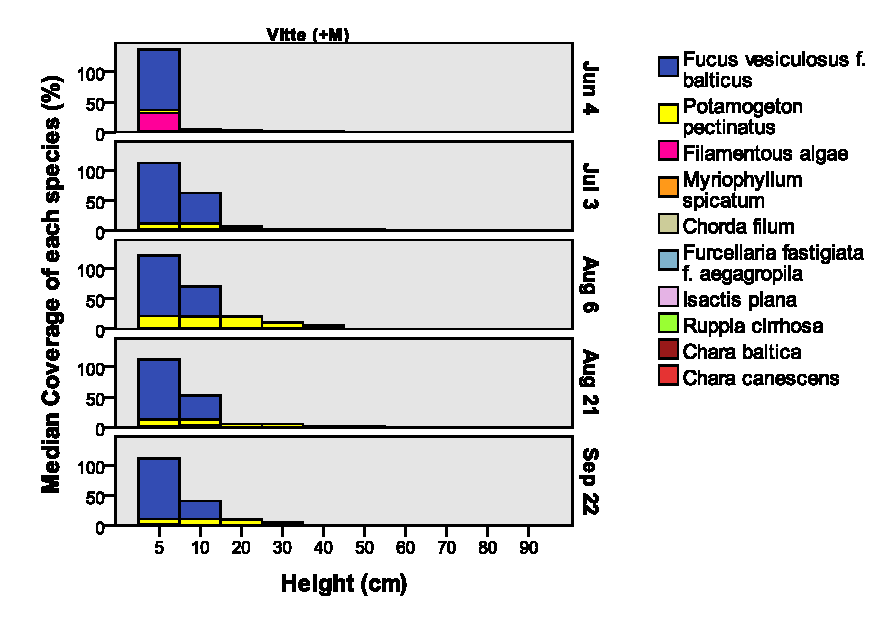
\includegraphics[width=0.90\textwidth]{images/Wuchshoehenkartierung/Vitte+Mb1.eps}
\caption[Höhenstufenkartierung Vitte (+M)]{Deckungen aller Arten auf Höhenstufen vom Grund bis zur Oberfläche, Vitte, dicht bewachsener Standort}
\label{fig:wuchshoehen_vitte_+m1}
\end{figure}
\\
\begin{figure}[!htb]
\centering
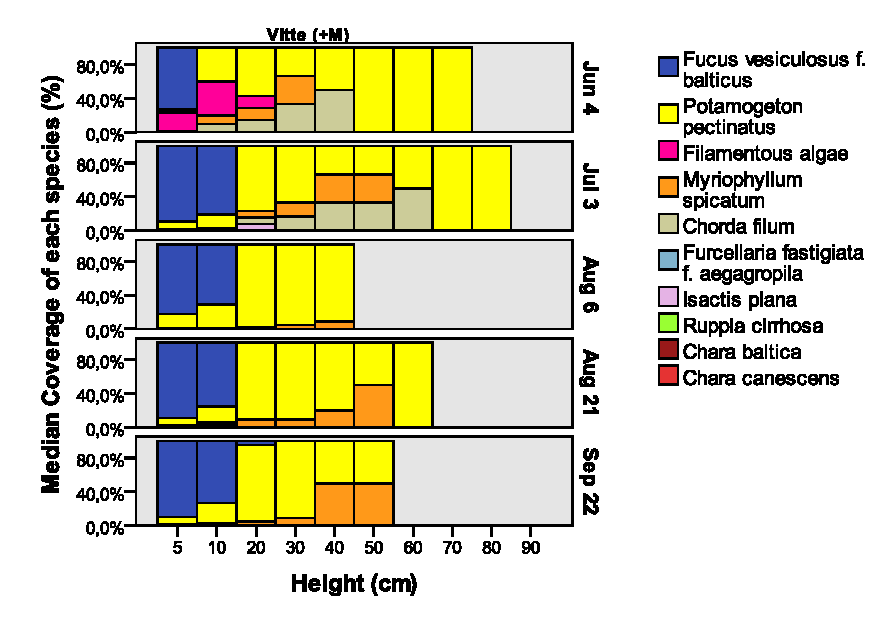
\includegraphics[width=0.90\textwidth]{images/Wuchshoehenkartierung/Vitte+Mb2.eps}
\caption[prozentuale Höhenstufenkartierung Vitte (+M)]{Prozentuale Deckungen aller Arten, bezogen auf die Gesamtdeckung auf jeder Höhenstufe, vom Grund bis zur Oberfläche, Vitte, dicht bewachsener Standort}
\label{fig:wuchshoehen_vitte_+m2}
\end{figure}

\FloatBarrier

\begin{figure}[!htb]
\centering
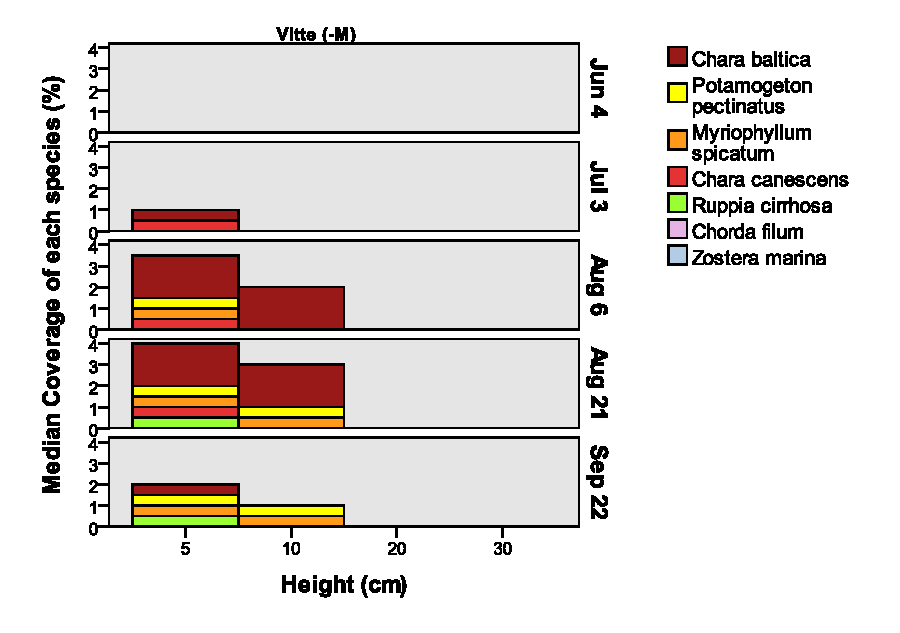
\includegraphics[width=0.90\textwidth]{images/Wuchshoehenkartierung/Vitte-M1.eps}
\caption[Höhenstufenkartierung Vitte (-M)]{Deckungen aller Arten auf Höhenstufen vom Grund bis zur Oberfläche, Vitte, spärlich bewachsener Standort}
\label{fig:wuchshoehen_vitte_-m1}
\end{figure}
\\
\begin{figure}[!htb]
\centering
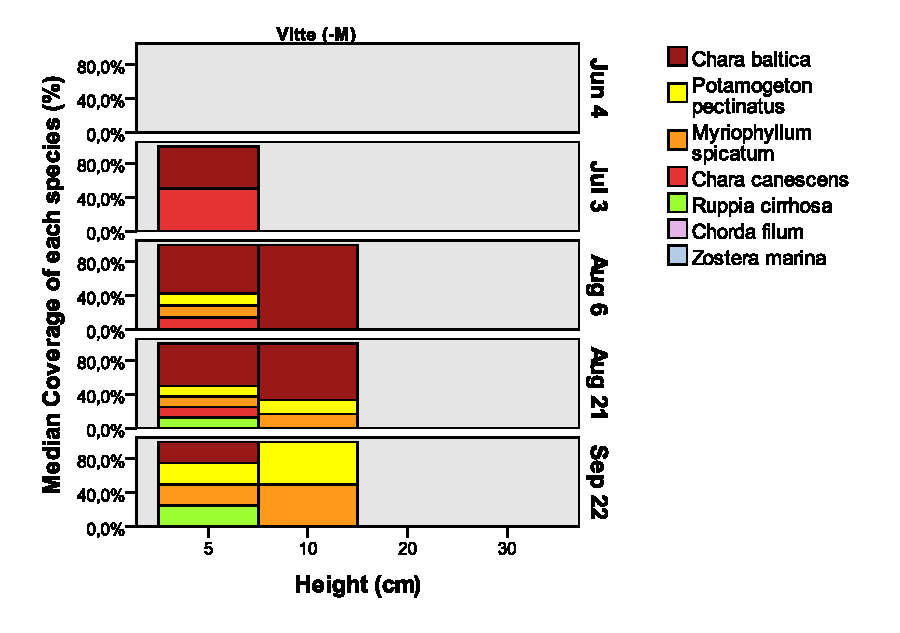
\includegraphics[width=0.90\textwidth]{images/Wuchshoehenkartierung/Vitte-M2.eps}
\caption[prozentuale Höhenstufenkartierung Vitte, vegetationsarmer Standort]{Prozentuale Deckungen aller Arten, bezogen auf die Gesamtdeckung auf jeder Höhenstufe vom Grund bis zur Oberfläche, Vitte, spärlich bewachsener Standort}
\label{fig:wuchshoehen_vitte_-m2}
\end{figure}
\\
\FloatBarrier


\subsubsection{Grieben, dicht bewachsener Standort}


\begin{figure}[!htb]
        \centering
        \begin{subfigure}[htb]{0.45\textwidth}
                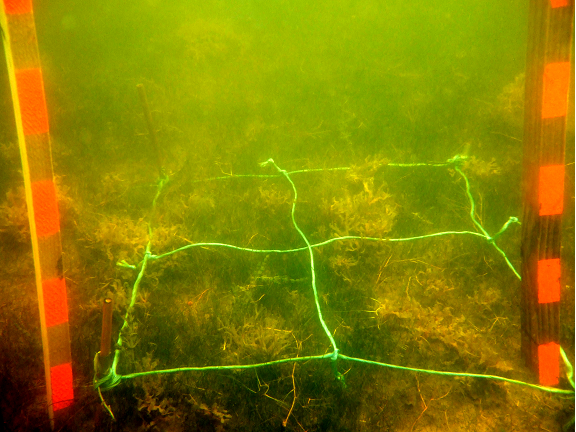
\includegraphics[width=\textwidth]{images/plotpictures/Bsp_G+M}
        \end{subfigure}
        \begin{subfigure}[htb]{0.45\textwidth}
                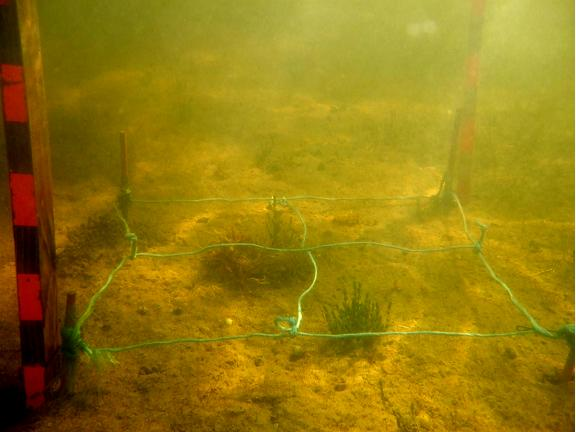
\includegraphics[width=\textwidth]{images/plotpictures/Bsp_G-M}
        \end{subfigure}
        \caption[Fotoaufnahmen der Vegetation in Grieben]{Vegetation in Grieben, vegetationsdominierter 						Standort (links) und  vegetationsarmer Standort (rechts), \unit{0,25}{\metre\squared}- 							Miniplots, Aufnahme August 2013}
        \label{fig:fotos_grieben}
\end{figure}

Die Vegetation am dicht bewachsenen Standort in Grieben ist sehr vielfältig. Im Verlauf der Wachstumssaisong wurden 11 Pflanzenarten kartiert, deren jeweiliges maximales Vorkommen sich abwechselt. Anfang Juni war der Standort zu \unit{30-50}{\%} bedeckt, davon machten ineinander verwobene, fädige Mikroalgen verschiedener Stämme und Arten mit \unit{20-40}{\%} den größten Anteil aus. Sie schwebten lose oder waren zwischen den Makrophyten verhakt. Die dominanten Makrophyten waren \textit{Ruppia cirrhosa} (\unit{10-20}{\%} Deckung) und \textit{Fucus vesiculosus} mit \unit{2-10}{\%} Deckung. An einem Plot war der Anteil von \textit{Fucus vesiculosus} mit \unit{40}{\%} höher. Außerdem wurden jeweils mit geringen Deckungsgraden die Arten \textit{Potamogeton pectinatus} und \textit{Myriophyllum spicatum} sowie \textit{Chara baltica} und \textit{Chorda filum} gefunden. Insgesamt nimmt die Deckung im Juni überhalb \unit{5}{\centri\metre} Höhe vom Grund stark ab. Ab \unit{20}{\centi\metre} Wuchshöhe kommen nur noch \textit{Potamogeton pectinatus} und die fadenförmige Alge \textit{Chorda filum} mit jeweiligen Deckungen unter einem Prozent vor.

Im Juli ging der Anteil filamentöser Algen stark zurück. Sie wurden ans Ufer gespült und starben dort ab. Die Bestände wurden nun hauptsächlich durch die rasig wachsende schraubige Salde \textit{Ruppia cirrhosa} (im Mittel \unit{40}{\%}Deckung)und durch \textit{Potamogeton pectinatus} (\unit{10-30}{\%} Deckung) gebildet. Während \textit{Ruppia cirrhosa} auf \unit{5}{\centi\metre}-Wuchshöhe beschränkt bleibt, ist \textit{Potamogeton pectinatus} deutlich aufgewachsen. Die Pflanzen verzweigen sich im unteren Bereich am Grund und das Volumen nimmt zur Oberfläche hin ab. Auf \unit{10 und 20} {\centi\metre} deckt \textit{Potamogeton pectinatus} durchschnittlich \unit{10 bzw. 2}{\%} der Fläche ab. Mit bis zu \unit{10}{\%} Deckung und bis zu \unit{20}{\centi\metre} tritt erstmals \textit{Chara horrida} im Juli auf.

Anfang August beträgt die Gesamtdeckung auf den Plots bereits \unit{60 bis 70}{\%}. Mit im Mittel \unit{30}{\%} Deckung hat sich \textit{Fucus vesiculosus f. balticus} ausgebreitet und ist bis auf \unit{30}{\centi\metre} vom Grund aufgewachsen. Er zeigt hier seine maximale Deckung. Auch die Bedeckung durch Characeen hat zugenommen. \textit{Chara baltica}, \textit{Chara horrida} und neu hinzugekommen \textit{Chara canescens} bedecken bis zu \unit{5}{\%} die Plots. Während sich \textit{Chorda filum} bereits zurückzog, erschien \textit{Chaetomorpha linum} neu auf den Flächen. Die losen, tellerartig ineinander verschlungenen fadenförmigen Algen wurden auf die Plots verdriftet. \textit{Myriophyllum spicatum} zeigte bei gleichbleibend geringer Gesamtdeckung von unter einem Prozent ihre maximale Wuchshöhe von bis zu \unit{40}{\centi\metre}.

Bis zum September breitete sich \textit{Ruppia cirrhosa} stark aus und bedeckte etwa \unit{60}{\%} der Flächen. Mit Ausnahme einer Aufnahmefläche, deren Gesamtdeckung sich auf \unit{40}{\%} reduzierte, waren die Flächen im September mit \unit{70-100}{\%} maximal mit Pflanzen bedeckt. Die Art blieb während des gesamten Untersuchungszeitraumes kleinwüchsig, selten über die \unit{5}{\centi\metre} Wuchshöhe hinauswachsend und sie bildete keine Fruchtstände. Auffällig war jedoch, dass sie Turionen ausgebildet hatte.

Die zweite Bestandbildende Art im September mit \unit{2-30}{\%} Deckung war \textit{Fucus vesiculosus}. Im Vergleich zum Juli befindet sich die Vegetation auf \unit{5}{\centi\metre} Wuchshöhe konzentriert, auf \unit{10}{\centi\metre} beträgt die Deckung durch Pflanzen lediglich \unit{5}{\%}. Die Characeen sowie \textit{Myriophyllum spicatum} und \textit{Potamogeton pectinatus} haben sich stark zurückgezogen. Neu erschienen sind Algenbüschel von \textit{Polysiphonia violacea}, die sich losgerissen zwischen den Pflanzen und sowie festgewachsen an der Schnur der Schwimmboje befanden. 



\subsubsection{Grieben, spärlich bewachsener Standort}


Zu Beginn der Felduntersuchungen im Juni waren die Flächen vollkommen vegetationsfrei. Bis zum August hat sich dies geändert: \textit{Fucus-vesiculosus}-Bällchen sind an den Standort gedriftet und verursachen Bedeckungen von \unit{2-10}{\%}. Daneben gibt es spärliche Bestände von \textit{Ruppia cirrhosa}, \textit{Chara canescens} und \textit{Chara baltica} mit jeweils unter einem bis zehn Prozent Deckung. \textit{Myriophyllum spicatum} und \textit{Potamogeton pectinatus} sind mit unter einem Prozent Deckung vertreten und wachsen am Höchsten (bis \unit{20}{\centi\metre}) auf. Im Mittel ist der Standort Anfang August zu \unit{5}{\%} mit Pflanzen bedeckt.

Die Vegetationsbedeckung nimmt im weiteren Jahresverlauf zu. Im September wurde die maximale Bedeckung von im Mittel \unit{30}{\%} beobachtet. Maximale und minimale Bedeckungen auf den Plots betrugen \unit{60 bzw. 10}{\%}. Der Anstieg des Anteils der Vegetation wird durch \textit{Fucus vesiculosus f. filiformis }verursacht, der vermehrt auf den Standort verdriftet wurde.\\



\begin{figure}[!htb]
\centering
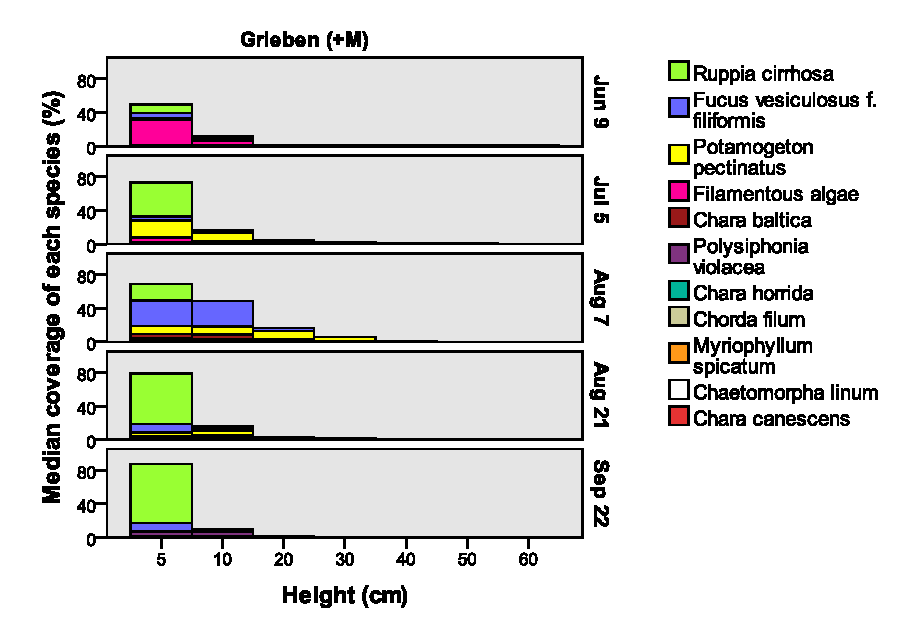
\includegraphics[width=0.90\textwidth]{images/Wuchshoehenkartierung/Grieben+M1.eps}
\caption[Höhenstufenkartierung Grieben (+M)]{Deckungen aller Arten auf Höhenstufen vom Grund bis zur Oberfläche, Grieben, dicht bewachsener Standort}
\label{fig:wuchshoehen_grieben_+m1}
\end{figure}
\\
\begin{figure}[!htb]
\centering
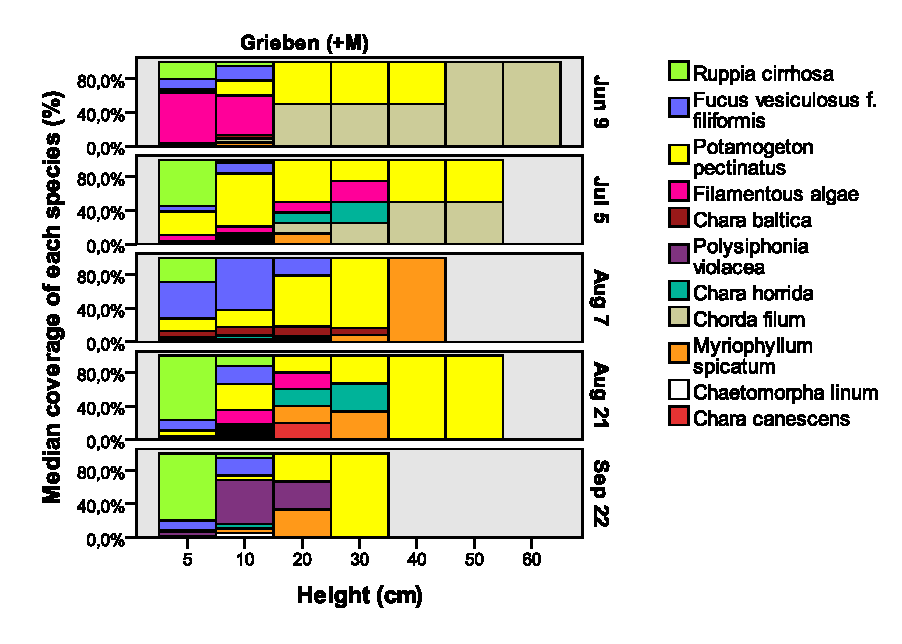
\includegraphics[width=0.90\textwidth]{images/Wuchshoehenkartierung/Grieben+M2.eps}
\caption[prozentuale Höhenstufenkartierung Grieben (+M)]{Prozentuale Deckungen aller Arten, bezogen auf die Gesamtdeckung auf jeder Höhenstufe, vom Grund bis zur Oberfläche, Grieben, dicht bewachsener Standort}
\label{fig:wuchshoehen_grieben_+m2}
\end{figure}

\FloatBarrier

\begin{figure}[!htb]
\centering
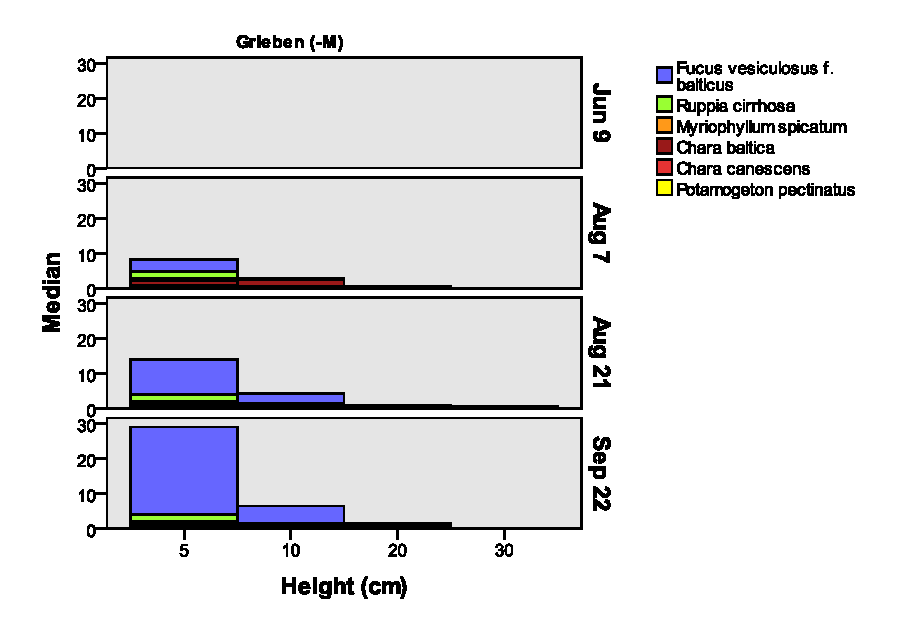
\includegraphics[width=0.90\textwidth]{images/Wuchshoehenkartierung/Grieben-M1.eps}
\caption[Höhenstufenkartierung Grieben (-M)]{Deckungen aller Arten auf Höhenstufen vom Grund bis zur Oberfläche, Grieben, spärlich bewachsener Standort}
\label{fig:wuchshoehen_grieben_-m1}
\end{figure}
\\
\begin{figure}[!htb]
\centering
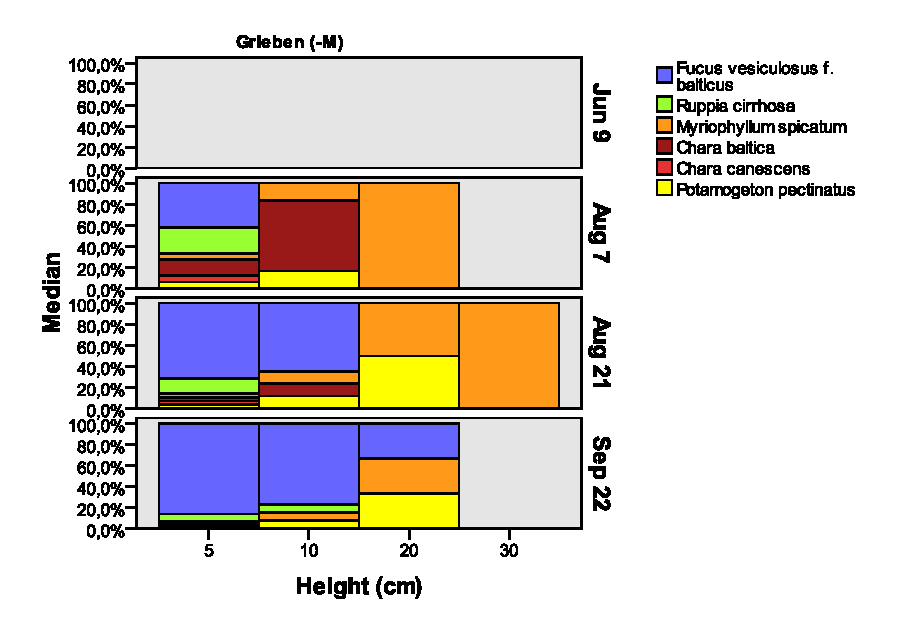
\includegraphics[width=0.90\textwidth]{images/Wuchshoehenkartierung/Grieben-M2.eps}
\caption[prozentuale Höhenstufenkartierung Grieben (-M)]{Prozentuale Deckungen aller Arten, bezogen auf die Gesamtdeckung auf jeder Höhenstufe, vom Grund bis zur Oberfläche, Grieben, spärlich bewachsener Standort}
\label{fig:wuchshoehen_grieben_-m2}
\end{figure}


\FloatBarrier


\subsection{Deckung und PVI}

Sowohl im Vitter Bodden als auch in der Griebener Bucht gab es ganzjährig einen Unterschied in der Bedeckung mit Phytobenthos zwischen den zu Beginn der Vegetationsperiode dicht und spärlich besiedelten Standorten.\\
Im Vitter Bodden war der Unterschied im Juni besonders groß. Die Plots waren vollständig bedeckt beziehungsweise komplett vegetationsfrei. Am vegetationsdominierten Standort verändert sich die Deckung im Jahresverlauf nicht, nur einmal im Juli ist aufgrund eines Ankerwurfes ein Loch in der \textit{Fucus vesiculosus}- dominierten Vegetationsdecke entstanden. Anfang August hatte sich die Decke durch den beweglichen \textit{Fucus} wieder geschlossen.
In der zu Beginn der Studie unbesiedelten Kontrollgruppe im Vitter Bodden hat sich bis Anfang August eine spärliche Vegetationsdecke mit einer mittleren Deckung von \unit{5}{\%} herausgebildet, welche sich bis Ende September aufrecht erhielt.

In der Griebener Bucht war der Unterschied in der Bedeckung zwischen den beiden Untersuchungsgruppen zu Beginn der Studie nicht so groß wie im Vitter Bodden. Die Gruppe auf der Ostseite der Bucht war im Juni vegetationsfrei und die andere zu \unit{30-40}{\%} mit Phytobenthos bedeckt. An beiden Standorten erhöhte sich die Deckung signifikant im Verlauf der Wachstumsperiode. Der dicht besiedelte Bereich war bereits im Juli zu \unit{60}{\%} mit Makrophyten bedeckt, bis Ende September stieg die Deckung allmählich auf \unit{90}{\%} an. Auf dem vorerst nicht besiedelten Bereich entwickelte sich bis Anfang August eine Bedeckung von \unit{5}{\%}. Bis Ende September stieg die Bedeckung auf \unit{30}{\%} an.

Nicht nur die Bedeckung mit Phytobenthos verändert sich im Jahresverlauf, sondern auch dessen Anteil an der Wassersäule. Neben der Wassertiefe, die als mehrjähriger Mittelwert in die Berechnung eingeht, nimmt die zunehmende Wuchshöhe einen Einfluss auf das PVI.

Obwohl das Wasser im Vitter Bodden im dicht besiedelten Bereich mit \unit{83}{\centi\metre} vergleichsweise tief ist, fanden sich hier deutlich höhere Anteile an Makrophytn in der Wassersäule. Im Juni waren es im Mittel \unit{7,7}{\%}. Bis Anfang August stieg der Anteil auf über \unit{15}{\%}. Der spärlich besiedelte Bereich ist mit \unit{62}{\centi\metre} flacher als der dicht besiedelte. Aufgrund der geringen Deckung und der geringen Wuchshöhe betrug das maximale PVI im August und im September \unit{0,6}{\%}. 

In der Griebener Bucht steigt das PVI im Verlauf der Wachstumssaisong in beiden Untersuchungsgruppen deutlich. Bei einer Wassertiefe von \unit{87}{\centi\metre} betrug der Anteil im dicht besiedelten Bereich im Juni \unit{2,4}{\%}. Anfang August erhöhte sich der Anteil auf \unit{7,1}{\%}. Bis zum September nimm das PVI leicht ab, jedoch bewegt sich diese Abnahme auf \unit{5,5}{\%} außerhalb des signifikanten Bereiches.
Der Spärlich besiedelte Bereich ist mit einer durchschnittlichen Tiefe von \unit{65}{\centi\metre} deutlich flacher als der dichtbesiedelte Bereich. Das PVI steigt hier im Verlauf der Wachstumssaisong auf \unit{1,2}{\%} im September an. Ende September gibt es keinen signifikanten Unterschied mehr zwischen dem PVI des dicht und des spärlich besiedelten Bereiches.


\begin{figure}[!htb]
\centering
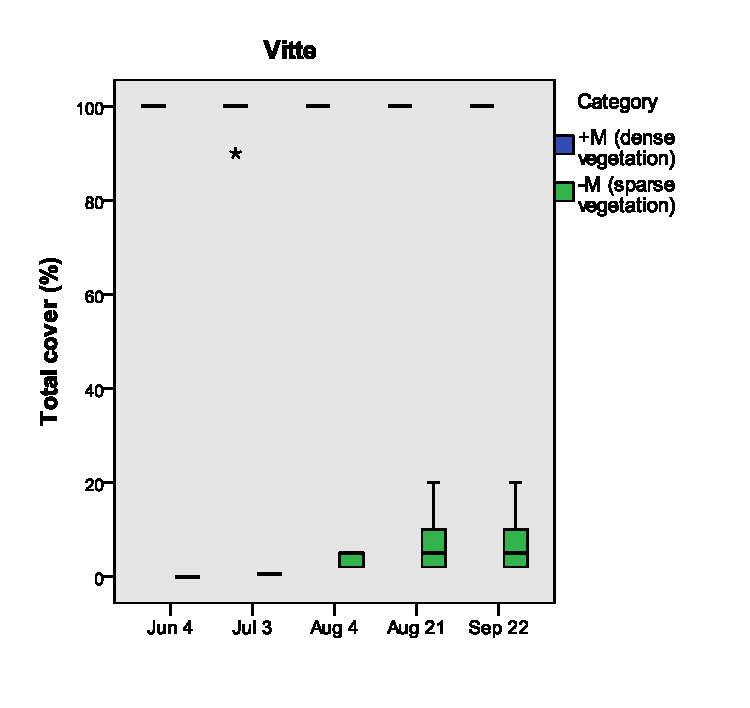
\includegraphics[width=0.70\textwidth]{images/total_cover/Boxplots_G_V1.eps}
\caption[Bedeckung mit Makrophyten, Vitte]{Bedeckung der Hauptuntersuchungs-Plots (\unit{4}{\metre\squared} im Vitter Bodden im Verlauf der Wachstumssaisong 2013}
\label{fig:cover_vitte}
\end{figure}

\begin{figure}[!htb]
\centering
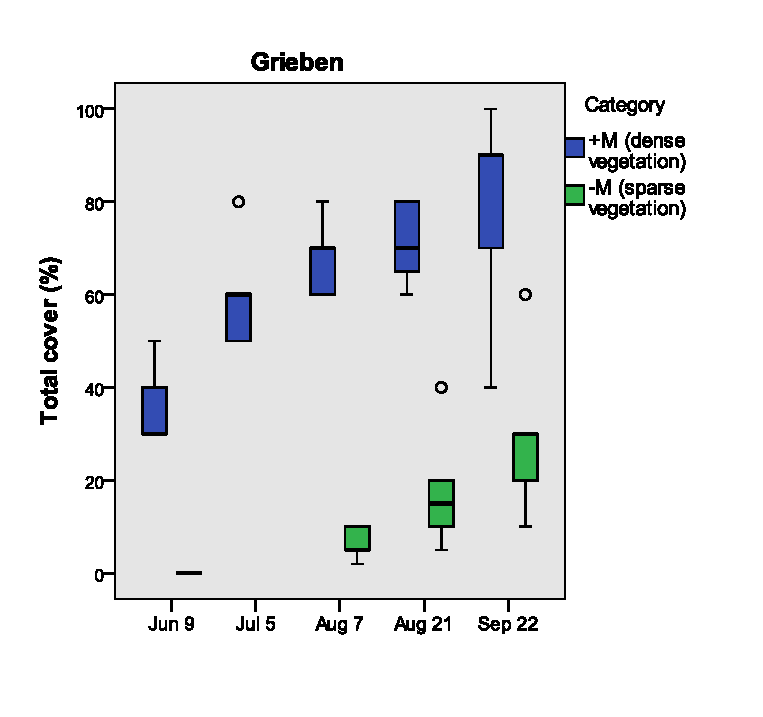
\includegraphics[width=0.70\textwidth]{images/total_cover/Boxplots_G_V2.eps}
\caption[Bedeckung mit Makrophyten, Grieben]{Bedeckung der Hauptuntersuchungs-Plots (\unit{4}{\metre\squared} in der Griebener Bucht im Verlauf der Wachstumssaisong 2013}
\label{fig:cover_grieben}
\end{figure}



\begin{figure}[!htb]
\centering
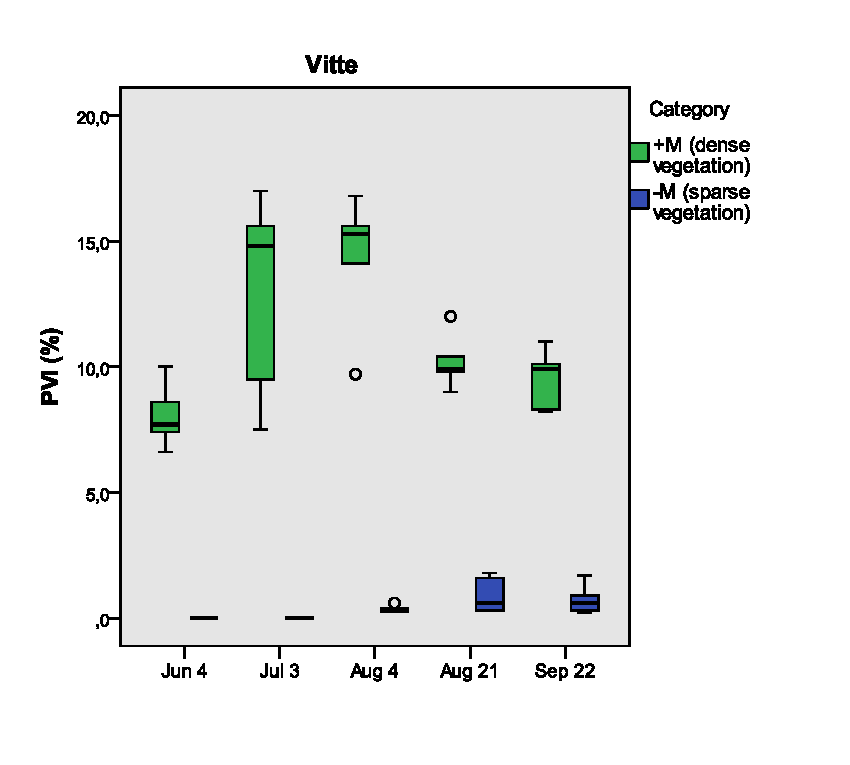
\includegraphics[width=0.70\textwidth]{images/pvi/boxplot_pvi1.eps}
\caption[PVI, Vitte]{Anteil des Phytobenthos an der Wassersäule (PVI nach \cite{jeppesen_1998}) im Vitter Bodden im Verlauf der Wachstumssaisong 2013}
\label{fig:pvi_vitte}
\end{figure}

\begin{figure}[!htb]
\centering
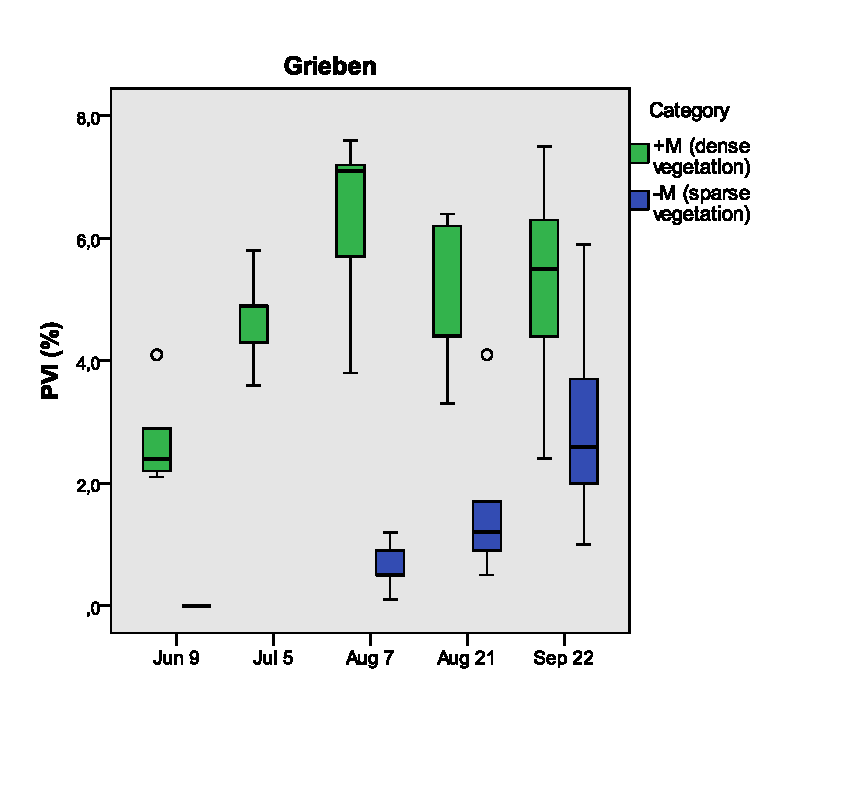
\includegraphics[width=0.70\textwidth]{images/pvi/boxplot_pvi2.eps}
\caption[PVI, Grieben]{Anteil des Phytobenthos an der Wassersäule (PVI nach \cite{jeppesen_1998}) in der Griebener Bucht im Verlauf der Wachstumssaisong 2013}
\label{fig:pvi_vitte}
\end{figure}

\FloatBarrier




\begin{table}[!htb]{\textwidth}
\centering
\caption[Teststatistik Unterschiede zwischen -M und +M in Grieben und Vitte]{Mann-Whithney-Teststatistik zur Ermittlung von Unterschieden in Deckung und PVI zwischen dicht und spärlich mit Phytobenthos besiedelten Standorten im Vitter Bodden und in der Griebener Bucht}
\begin{tabular}{lrrrrrr}
\toprule

Location					& Date		& \multicolumn{2}{c}{Total Cover} 	& \multicolumn{2}{c}{PVI}\\
\midrule
							&	& \multicolumn{1}{c}{Z} & \multicolumn{1}{c}{\textit{p}}& \multicolumn{1}{c}{Z}	& \multicolumn{1}{c}{\textit{p}}\\
\midrule
\multirow{5}{*}{Vitter Bodden}& Jun 04 	& -3.000 		& 0.008\ast			& -2.785			& 0.008\ast\\
 							& Jul 03    & -2.887	    & 0.008\ast 		& -2.783			& 0.008\ast\\
							& Aug 04	& -2.835		& 0.008\ast	     	& -2.643 			& 0.008\ast\\
							& Aug 21	& -2.798 		& 0.008\ast		    & -2.619			& 0.008\ast\\
							& Sep 22	& -2.795 		& 0.008\ast			& -2.611			& 0.008\ast\\
\midrule
\multirow{5}{*}{Griebener Bucht}& Jun 09& -2.825		& 0.008\ast		    & -2.785		& 0.008\ast\\
							& Aug 07	& -2.643		& 0.008\ast		    & -2.619		& 0.008\ast\\
							& Aug 21	& -2.619		& 0.008\ast		    & -2.410		& 0.016\ast\\
							& Sep 22	& -2.417		& 0.016\ast		    & -1.567		& 0.151\\
							
\bottomrule
\end{tabular}
\label{tab:mann_whithney_v,g}
\end{table}



\begin{table}[!htb]{\textwidth}
\centering
\caption[Deskriptive Statistik, Deckung und PVI in Grieben und Vitte]{Deskriptive Statistik zu Deckung und PVI in Vitter Bodden und Griebener Bucht; +M = dichte Vegetation, -M = spärliche Vegetation, MAD = Mittlere Abweichung vom Median}
\begin{tabular}{lrrrrr}
\toprule
Location & \multicolumn{1}{c}{Date}	& \multicolumn{2}{c}{Total Cover} 	& \multicolumn{2}{c}{PVI}\\
\midrule
							&			& Median 		& MAD				& Median		& MAD\\
\midrule
\multirow{5}{*}{Vitter Bodden (+M)} & Jun 04 	& 100.00 		& 0.00				& 7.70			& 0.92\\
 							& Jul 03    & 100.00	    & 2.00				& 14.80			& 3.12\\
							& Aug 04	& 100.00		& 0.00				& 15.30			& 1.72\\
							& Aug 21	& 100.00		& 0.00				& 9.90			& 0.72\\
							& Sep 22	& 100.00		& 0.00				& 9.90			& 0.92\\
\midrule
\multirow{5}{*}{Vitter Bodden (-M)} & Jun 04	& 0.00			& 0.00				& 0.00			& 0.00\\
							& Jul 03	& 0.00			& 0.00				& 0.00			& 0.00\\
							& Aug 06	& 5.00			& 1.20				& 0.30			& 0.08\\
							& Aug 21	& 5.00			& 5.20				& 0.60			& 0.56\\
							& Sep 22	& 5.00			& 5.20				& 0.60			& 0.42\\
\midrule
\multirow{5}{*}{Griebener Bucht (+M)}& Jun 09	& 30.00			& 6.00				& 2.42			& 0.54\\
							& Jul 05	& 60.00			& 8.00				& 4.90			& 0.56\\
							& Aug 07	& 70.00			& 6.00				& 7.10			& 1.06\\
							& Aug 21	& 70.00			& 7.00				& 4.40			& 0.98\\
							& Sep 22	& 90.00			& 16.00				& 5.50			& 1.40\\
\midrule	
\multirow{4}{*}{Griebener Bucht (-M)}& Jun 09	& 0.00			& 0.00				& 0.00			& 0.00\\
							& Aug 07	& 5.00			& 2.60				& 0.50			& 0.30\\
							& Aug 21	& 15.00			& 9.00				& 1.20			& 0.88\\
							& Sep 22	& 30.00			& 12.00				& 2.60			& 1.32\\
\bottomrule
\end{tabular}
\label{tab:statistik_G,V_Deckung,PVI}
\end{table}

\FloatBarrier


\begin{table}[!htb]{\textwidth}
\centering
\caption[Teststatistik Unterschiede in der Deckung im Jahresverlauf in Grieben und Vitte]{Kruskal-Wallis-Teststatistik zur Ermittlung von Unterschieden in der Bedeckung mit Phytobenthos im Jahresverlauf sowie Multiple Vergleiche mit dem Dunn's Test bei Signifikanz (\textit{p} < 0,05; Kennzeichnung mit Stern) im Vitter Bodden und in der Griebener Bucht}
\begin{tabular}{lrcrlr}

\toprule

Location & \multicolumn{3}{c}{Kruskal Wallis Test} 	& \multicolumn{2}{c}{Dunn's Multiple Comparisons Test}\\
\midrule
& \multicolumn{1}{c}{\chi\squared} & df & \multicolumn{1}{c}{\textit{p}-Value} & \multicolumn{1}{c}{Date} & \multicolumn{1}{c}{\textit{p}-Value}\\
&&& (Asymptotic) && \multicolumn{1}{c}{(Adjusted)}\\
\midrule
Vitte (+M)	& 4.000 & 4 & 0.406 \\
\midrule
\multirow{10}{*}{Vitter Bodden (-M)}	& 19.384 & 4 & 0.001\ast & Jun 4 vs. Jul 03 & > 0.999\\
														&&&& Jun 04 vs. Aug 06 & 0.025\ast\\
														&&&& Jun 04 vs. Aug 21& 0.006\ast\\
														&&&& Jun 04 vs. Sep 22&	0.006\ast\\
														&&&& Jul 03 vs. Aug 06&	0.540\\
														&&&& Jul 03 vs. Aug 21&	0.203\\
														&&&& Jul 03 vs. Sep 22&	0.203\\
														&&&& Aug 06 vs. Aug 21&	> 0.999\\
														&&&& Aug 06 vs. Sep 22&	> 0.999\\
														&&&& Aug 21 vs. Sep 22&	> 0.999\\
\midrule
\multirow{10}{*}{Griebener Bucht (+M)} & 13.283 & 4 & 0.010\ast & Jun 09 vs. Jul 05 & 0.906\\
															&&&& Jun 09 vs. Aug 07 & 0.119\\
															&&&& Jun 09 vs. Aug 21 & 0.048\ast\\
															&&&& Jun 09 vs. Sep 22 & 0.001\ast\\
															&&&& Jul 05 vs. Aug 07 & > 0.999\\
															&&&& Jul 05 vs. Sep 22 & > 0.999\\
															&&&& Aug 07 vs. Aug 21 & > 0.999\\
															&&&& Aug 07 vs. Sep 22 & > 0.999\\
															&&&& Aug 21 vs. Sep 22 & > 0.999\\
\midrule
\multirow{6}{*}{Griebener Bucht (-M)} & 15.112 & 3 & 0.002\ast & Jun 09 vs. Aug 07	& 	0.624\\
															&&&& Jun 09 vs. Aug 21	&	0.025\ast\\
															&&&& Jun 09 vs. Sep 22	&	0.002\ast\\
															&&&& Aug 07 vs. Aug 21	&	> 0.999\\
															&&&& Aug 07 vs. Sep 22	&	0.270\\
															&&&& Aug 21 vs. Sep 22	&	> 0.999\\
															
\bottomrule
\end{tabular}
\label{tab:kruskal_wallis_deckung_v,g}
\end{table}





\begin{table}[!htb]{\textwidth}
\centering
\caption[Teststatistik: Unterschiede des PVI im Jahresverlauf in Grieben und Vitte]{Kruskal-Wallis-Teststatistik zur Ermittlung von Unterschieden im Anteil des Phytobenthos an der Wassersäule (PVI) sowie Multiple Vergleiche mit dem Dunn's Test bei Signifikanz (\textit{p} < 0,05, Kennzeichnung mit Stern)im Vitter Bodden und in der Griebener Bucht}
\begin{tabular}{lrcrlr}

\toprule

Location & \multicolumn{3}{c}{Kruskal Wallis Test} 	& \multicolumn{2}{c}{Dunn's Multiple Comparisons Test}\\
\midrule
& \multicolumn{1}{c}{\chi\squared} & df & \multicolumn{1}{c}{\textit{p}-Value} & \multicolumn{1}{c}{Date} & \multicolumn{1}{c}{\textit{p}-Value}\\
&&& (Asymptotic) && (Adjusted)\\
\midrule
Vitte (+M)	& 4.000 & 4 & 0.406 \\
\midrule
\multirow{10}{*}{Vitter Bodden (+M)} & 9.836 & 4 & 0.043\ast & Jun 04 vs. Jul 03 & 0.269\\
&&&& Jun 04 vs. Aug 06	&	0.032\ast\\
&&&& Jun 04 vs. Aug 21	&	> 0.999\\
&&&& Jun 04 vs. Sep 22	&	> 0.999\\
&&&& Jul 03 vs. Aug 06	&	> 0.999\\
&&&& Jul 03 vs. Aug 21	&	> 0.999\\
&&&& Jul 03 vs. Sep 22	&	> 0.999\\
&&&& Aug 06 vs. Aug 21	&	> 0.999\\
&&&& Aug 06 vs. Sep 22	&	0.780\\
&&&& Aug 21 vs. Sep 22	&	> 0.999\\													
\midrule
\multirow{10}{*}{Vitter Bodden (-M)} & 19.276 & 4 & 0.025\ast & Jun 04 vs. Jul 03 &	> 0.999\\
&&&& Jun 04 vs. Aug 06	&	0.157\\
&&&& Jun 04 vs. Aug 21	&	0.019\ast\\
&&&& Jun 04 vs. Sep 22	&	0.042\ast\\
&&&& Jul 03 vs. Aug 06	&	0.157\\
&&&& Jul 03 vs. Aug 21	&	0.019\ast\\
&&&& Jul 03 vs. Sep 22	&	0.042\ast\\
&&&& Aug 06 vs. Aug 21	&	> 0.999\\
&&&& Aug 06 vs. Sep 22	&	> 0.999\\
&&&& Aug 21 vs. Sep 22	&	> 0.999\\
\midrule
\multirow{10}{*}{Griebener Bucht (+M)} & 11.164 & 4 & 0.025\ast & Jun 09 vs. Jul 05 & 0.613\\
															&&&& Jun 09 vs. Aug 07 & 0.014\ast\\
															&&&& Jun 09 vs. Aug 21 & 0.332\\
															&&&& Jun 09 vs. Sep 22 & 0.180\\
															&&&& Jul 05 vs. Aug 07 & > 0.999\\
															&&&& Jul 05 vs. Sep 22 & > 0.999\\
															&&&& Aug 07 vs. Aug 21 & > 0.999\\
															&&&& Aug 07 vs. Sep 22 & > 0.999\\
															&&&& Aug 21 vs. Sep 22 & > 0.999\\
\midrule
\multirow{6}{*}{Griebener Bucht (-M)} & 14.926 & 3 & 0.002\ast & Jun 09 vs. Aug 07	& 	0.565\\
															&&&& Jun 09 vs. Aug 21	&	0.035\ast\\
															&&&& Jun 09 vs. Sep 22	&	0.002\ast\\
															&&&& Aug 07 vs. Aug 21	&	> 0.999\\
															&&&& Aug 07 vs. Sep 22	&	0.275\\
															&&&& Aug 21 vs. Sep 22	&	> 0.999\\
															
\bottomrule
\end{tabular}
\label{tab:kruskal_wallis_pvi_v,g}
\end{table}
\\
\\
\\
\\
\\

\FloatBarrier


\subsection{Biomasse}

Bereits Anfang Juli gab es im Vitter Bodden auf den vegetationsdominierten Untersuchungsflächen im Mittel Biomassewerte von \unit{558}{\gram\per\metre\squared} Trockensubstanz. Dabei ist die mittlere Abweichung vom Median recht groß, auf einer Untersuchungsfläche fanden sich sogar etwa \unit{800}{\gram\per\metre\squared}. Bis zum August erhöht sich die Biomasse auf den Plots auf im Mittel \unit{890}{\gram\per\metre\squared}. Es gibt einen deutlichen Unterschied zu der vegetationsarmen Untersuchungsgruppe. Hier gab es im Mittel \unit{15}{\gram\per\metre\squared} Trocken-Biomasse im August. Etwa gleich viel (\unit{16,5}{\gram\per\metre\squared}) fanden sich auch in der Griebener Bucht im spärlich bewachsenen Bereich. 

Auch die Biomasse in der Griebener Bucht unterscheidet sich signifikant zwischen den beiden Untersuchungsgruppen, jedoch waren hier die Biomassewerte im dicht bewachsenen Bereich von im Mittel \unit{132}{\gram\per\metre\squared} im Juli und \unit{126}{\gram\per\metre\squared} im August  deutlich geringer als die des dicht bewachsenen Bereiches im \textit{Fucus vesiculosus }-dominierten Vitter Bodden. Es gab hier keine signifikante Zunahme der Biomasse von Anfang Juli bis Anfang August.

Der Organische Gehalt der Biomasse unterscheidet sich zwischen den Standorten im Vitter Bodden \unit{60-68}{\gram\per\metre\squared} und in der Griebener Bucht \unit{80-81}{\gram\per\metre\squared}. Es gibt jedoch jeweils keine signifikanten Unterschiede zwischen den vegetationsarmen und vegetationsreichen Untersuchungsgruppen.


\begin{figure}[!htb]
\centering
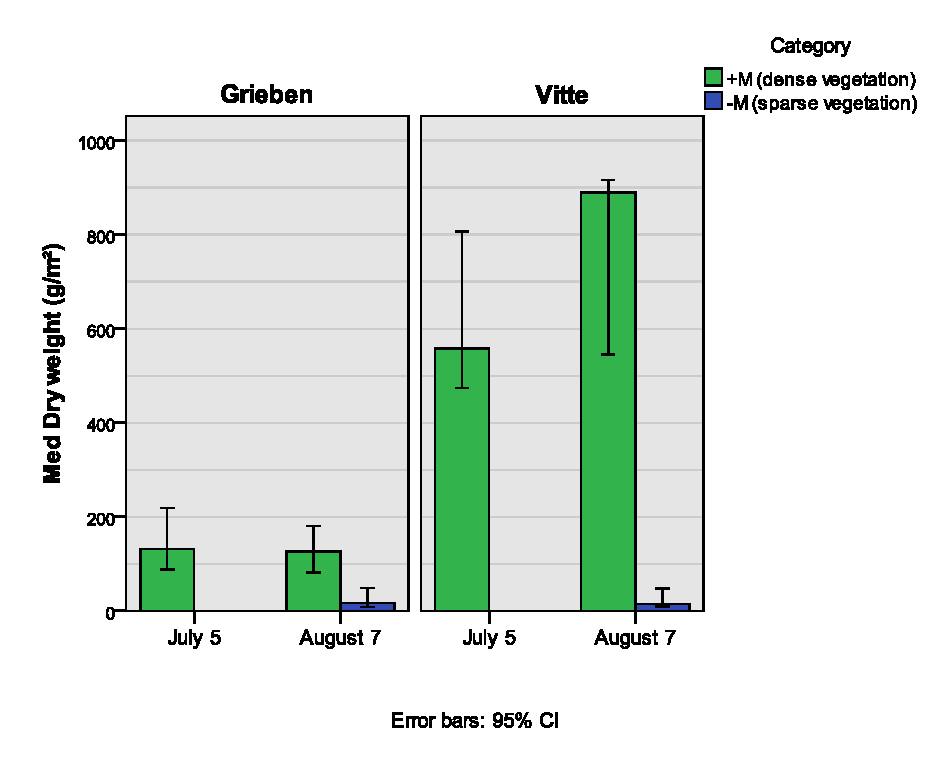
\includegraphics[width=0.80\textwidth]{images/biomass/biomasse_berichtigt1.eps}
\caption[Biomasse an den Hiddenseer Standorten]{Biomasse (Trockengewicht) geerntet auf Miniplots (\unit{0,25}{\metre\squared} neben den Hauptuntersuchungsplots in Grieben und Vitte, Probenahme Anfang Juli (nur dicht bewachsene Standorte) und Anfang August (dicht und spärlich bewachsene Standorte); Median (Balken) und \unit{95}{\%}-Bereich(Antennen) der Daten von jeweils 5 Replikaten}
\label{fig:biomasse}
\end{figure}

\begin{figure}[!htb]
\centering
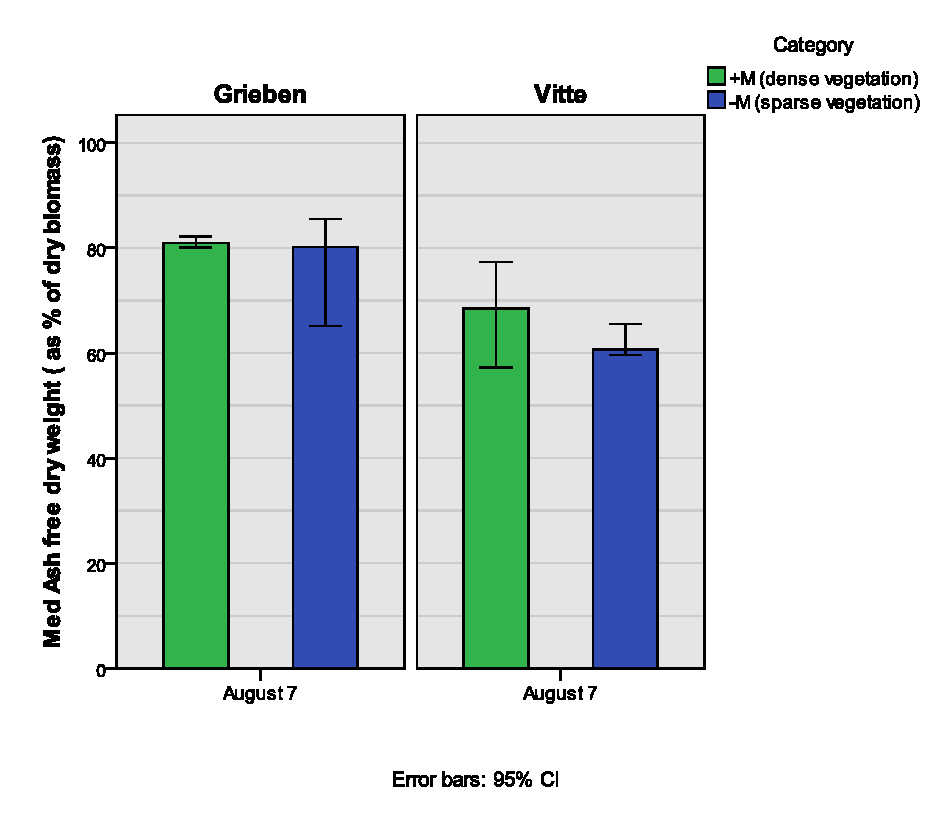
\includegraphics[width=0.80\textwidth]{images/biomass/biomasse_afdg_berichtigt1.eps}
\caption[Organischer Anteil der Biomasse an den Hiddenseer Standorten]{Organischer Anteil (ermittelt als aschfreies Trockengewicht) der Biomasse auf den Miniplots (\unit{0,25}{\metre\squared} in Grieben und Vitte, Probenahme Anfang August; Median (Balken) und \unit{95}{\%}-Bereich(Antennen) der Daten von jeweils 5 Replikaten}
\label{fig:biomasse_verascht}
\end{figure}


\FloatBarrier
\\


\begin{table}[!htb]{\textwidth}
\centering
\caption[Deskriptive Statistik, Biomasse und deren organischer Gehalt in Grieben und Vitte]{Deskriptive Statistik zur Biomasse (Dry Weight, Trockengewicht) und Organischer Gehalt (AFDW) im Vitter Bodden und in der Griebener Bucht; +M = dichte Vegetation, -M = spärliche Vegetation, MAD = Mittlere Abweichung vom Median}
\begin{tabular}{llrrrr}
\toprule
Location & Date	& \multicolumn{2}{c}{Dry Weight} 	& \multicolumn{2}{c}{AFDW}\\
&& \multicolumn{2}{c}{(\gram\per\metre\squared)} & \multicolumn{2}{c}{(\%)}\\
\midrule
							&			& Median 		& MAD				& Median		& MAD\\
\midrule
\multirow{2}{*}{Vitter Bodden (+M)}& July 	& 558.48		& 100.92			\\
 								 & August	& 890.28		& 119.74			& 68.47			& 4.77\\
\midrule
\multirow{1}{*}{Vitter Bodden (-M)}& August & 15.08			& 9.42				& 60.70			& 1.35\\
\midrule
\multirow{2}{*}{Griebener Bucht (+M)}& July & 132.12		& 30.81				\\
									& August & 126.48		& 36.50				& 80.95			& 0.62\\
\midrule	
\multirow{1}{*}{Griebener Bucht (-M)}& August & 16.52		& 9.23				& 80.16			& 5.94\\
\bottomrule
\end{tabular}
\label{tab:statistik_biomasse}
\end{table}

\FloatBarrier


\subsection{Sediment}



\begin{table}[!htb]{\textwidth}
\centering
\caption[Deskriptive Statistik, Korngrößenverteilung in Grieben und Vitte]{Deskriptive Statistik zu den Korngrößenverteilungen im Vitter Bodden (V) und in der Griebener Bucht (G); +M = dichte Vegetation, -M = spärliche Vegetation, MD = Median, MAD = Mittlere Abweichung vom Median, die Schiefe (Skewness) bezieht sich auf die Phi-Korngrößen}
\begin{tabular}{ccrrrrrrrrrr}
\toprule
Location & \multicolumn{1}{c}{Date}	& \multicolumn{2}{c}{MD Grain} 	& \multicolumn{2}{c}{Sorting} & \multicolumn{2}{c}{Skewness} & \multicolumn{2}{c}{\unit{< 63}{\mu\metre}} & \multicolumn{2}{c}{AFDW}\\
&& \multicolumn{2}{c}{Size ($ \phi $)} &&&&& \multicolumn{2}{c}{(\%)} & \multicolumn{2}{c}{(\%)}\\
\midrule
                      && MD	& MAD	& MD	&	MAD		& MD	&	MAD		& MD	&	MAD	& 	MD	&	MAD\\
\midrule
\multirow{3}{*}{V (+M)}	& Jul 05 & 2.13 & &0.54 &&&&6.04 &&1.23\\
						& Aug 01 & 2.37 & 0.03 & 0.93 & 0.07 & 0.10 & 0.05 & 9.05 & 1.79 & 1.43 & 0.41\\
						& Aug 19 & 2.08 & 0.16 & 0.93 & 0.02 & 0.22 & 0.09 & 8.61 & 0.60 & 1.70 & 0.28\\
\midrule
\multirow{3}{*}{V (-M)}	& Jul 05 & 2.69 & 	   & 0.56 &      & 	    & 	   & 5.56 &	     & 0.91\\
						& Aug 01 & 2.10 & 0.14 & 0.74 & 0.06 & 0.15 & 0.10 & 4.24 & 0.97 & 0.79 & 0.15\\
						& Aug 19 & 2.1 & 0.08 & 0.74 & 0.06 & 0.18 & 0.03 & 4.11 & 1.15 & 0.95 & 0.15\\
\midrule
\multirow{3}{*}{G (+M)}	& Jun 11 & 3.65 & 0.04 & 0.94 & 0.13 & -0.16 & 0.08 & 32.05 & 2.77 & 4.77 & 0.42\\
						& Jul 30 & 3.61 & 0.96 & 0.95 & 0.31 & -0.17 & 0.05 & 28.31 & 3.09 & 4.19 & 0.44\\
						& Aug 17 & 3.63 & 0.06 & 1.11 & 0.19 & -0.29 & 0.11 & 30.15 & 3.57 & 4.18 & 0.20\\
\midrule
\multirow{3}{*}{G (-M)} & Jun 11 & 3.47 & 0.02 & 0.66 & 0.03 & -0.09 & 0.03 & 11.95 & 1.06 & 1.69 & 0.24\\
						& Jul 30 & 3.42 & 0.11 & 0.67 & 0.04 & -0.13 & 0.08 & 10.23 & 1.30 & 1.43 & 0.06\\
						& Aug 17 & 3.47 & 0.89 & 0.66 & 0.18 & -0.09 & 0.03 & 14.38 & 4.92 & 1.65 & 0.16\\		
						
\bottomrule
\end{tabular}
\label{tab:statistik_G,V_sedimentparameter}
\end{table}





\subsubsection{Vitte, dicht bewachsener Standort}

Das Sediment auf diesen Untersuchungsflächen ändert sich nicht signifikant im Jahresverlauf in Hinsicht auf den Median der Korngrößenverteilung, die Sortierung und die Schiefe. Mit einem Anteil von \unit{40-50}{\%} beziehungsweise von \unit{30-40}{\%} dominieren die Anteile von feinem Sand (\unit{2-3}{$\phi$}) und Mittelsand (\unit{1-2}{$\phi$}). Der Median der Korngröße beträgt \unit{2,08-2,13}{$\phi$}. Das Sediment ist mäßig gut sortiert und zeigt eine positive Schiefe, das heißt, der Median der Verteilungskurve ist nach rechts in den grobkörnigeren Bereich (auf der $\phi$- Verteilungskurve nach links) verschoben. Der Anteil der \unit{< 63}{\mu\metre}-Fraktion, welche den Silt- und Tongehalt repräsentiert, beträgt im Juli \unit{6}{\%} und im August \unit{8,6-9}{\%}, die Zunahme ist jedoch nicht signifikant. Etwa gleich viel sehr feiner Sand (3-4 $\phi$) ist enthalten, während der Gehalt an Grobsanden und sehr groben Sanden vernachlässigbar ist. Der organische Gehalt des Sedimentes beträgt zwischen \unit{1,2}{\%} im Juli und \unit{1,7}{\%} Ende August. Die Zunahme des organischen Gehaltes in der Vegetationsperiode ist nicht signifikant.

\begin{figure}[!htb]
\centering
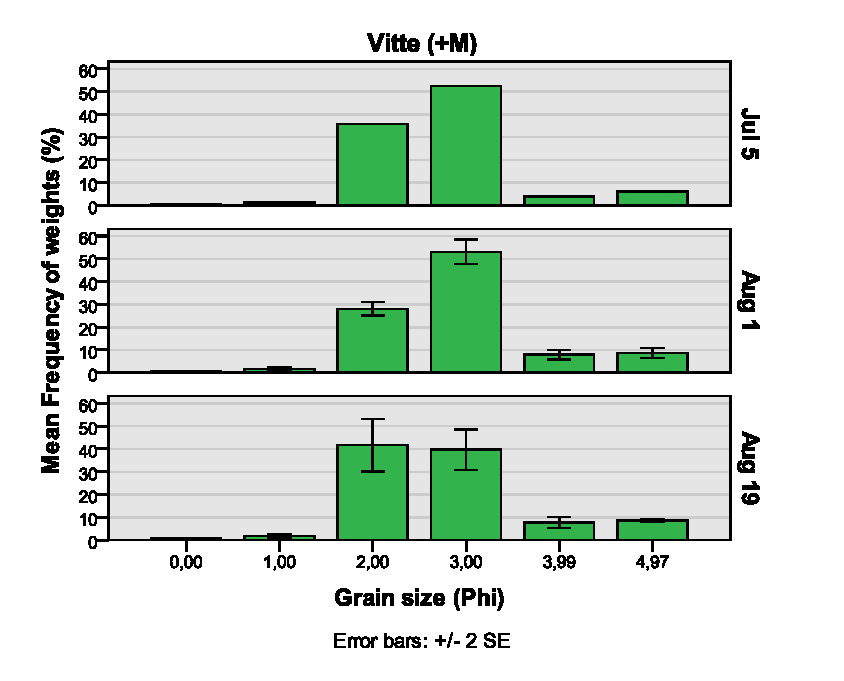
\includegraphics[width=0.70\textwidth]{images/grainsize/sediment_im_jahr1.eps}
\caption[Korngrößenverteilungen Vitte (+M)]{Korngrößenverteilungen am dicht bewachsenen Standort im Vitter Bodden; Juli: 3 Messparallelen aus einem Kern, August: Messparallelen aus 5 Sedimentkernen}
\label{fig:korngrössen_Vitte_+m}
\end{figure}



\subsubsection{Vitte, spärlich bewachsener Standort}

Die Sedimente an dieser Untersuchungsgruppe unterscheiden sich von denen auf den dicht bewachsenen Untersuchungsflächen im Vitter Bodden, jedoch mit Ausnahme des organischen Gehaltes, welcher im Mittel \unit{0,8-1}{\%} betrug. Die Verteilungskurve ist mäßig bis schlecht sortiert und ebenfalls in den grobkörnigen Bereich verschoben. Die Mittelsand und Feinsandanteile dominieren und nehmen zusammen über \unit{90}{\%} des Gesamtprobenmaterials ein. Sowohl grobe als auch sehr feine Sande sind kaum vorhanden und auch der Ton-und Silt-Anteil ist mit ca. \unit{4}{\%} etwas geringer. Das Verhältnis von Mittelsand zu Feinsand ist hier umgekehrt. Der Mittelsand hat einen größeren Anteil von etwa \unit{50}{\%} während der Feinsand einen geringeren Anteil von etwa \unit{40-45}{\%} hat. 


\begin{figure}[!htb]
\centering
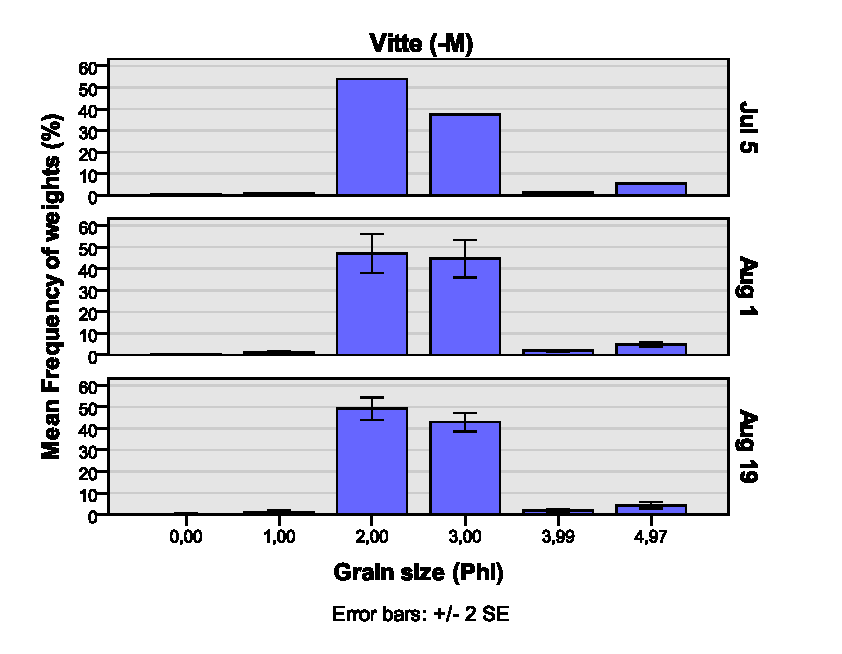
\includegraphics[width=0.70\textwidth]{images/grainsize/sediment_im_jahr2.eps}
\caption[Korngrößenverteilungen Vitte (-M)]{Korngrößenverteilungen am spärlich bewachsenen Standort im Vitter Bodden; Juli: 3 Messparallelen aus einem Kern, August: Messparallelen aus 5 Sedimentkernen}
\label{fig:korngrössen_Vitte_-m}
\end{figure}


\subsubsection{Grieben, dicht bewachsener Standort}

Die Sedimente auf den Flächen dieser Untersuchungsgruppe sind mäßig bis schlecht sortiert und zeigen eine negative Schiefe aufgrund der Dominanz der feinen Korngrößenfraktionen. Mit etwa \unit{50-52}{\%} ist sehr feiner Sand (3-4 $\phi$) am stärksten vertreten. Auch der Ton- und Siltanteil ist mit \unit{30-35}{\%} sehr hoch. Der Median der Korngröße beträgt im Mittel \unit{3,6}{$\phi$} und verringert sich zwischen Juni und Juli leicht im Jahresverlauf. Insgesamt verschiebt sich das Verteilungsmuster im Verlauf der Vegetationsperiode leicht in den feinkörnigeren Bereich. Mittelsand und Feinsand sind insgesamt mit nur etwa \unit{5 bzw 8}{\%} vertreten. Im Vergleich zu den Vitter Untersuchungsgruppen gab es eine geringe Menge (etwa \unit{2-6}{\%} sehr groben Sand beziehungsweise Kiessteinchen oder Muschelschalenreste. 
Der Organische Anteil des Sedimentes beträgt im Mittel \unit{0,2-0,4}{\%} und entspricht damit dem organischen Gehalt des vegetationsfreien Standortes im Vitter Bodden.



\begin{figure}[!htb]
\centering
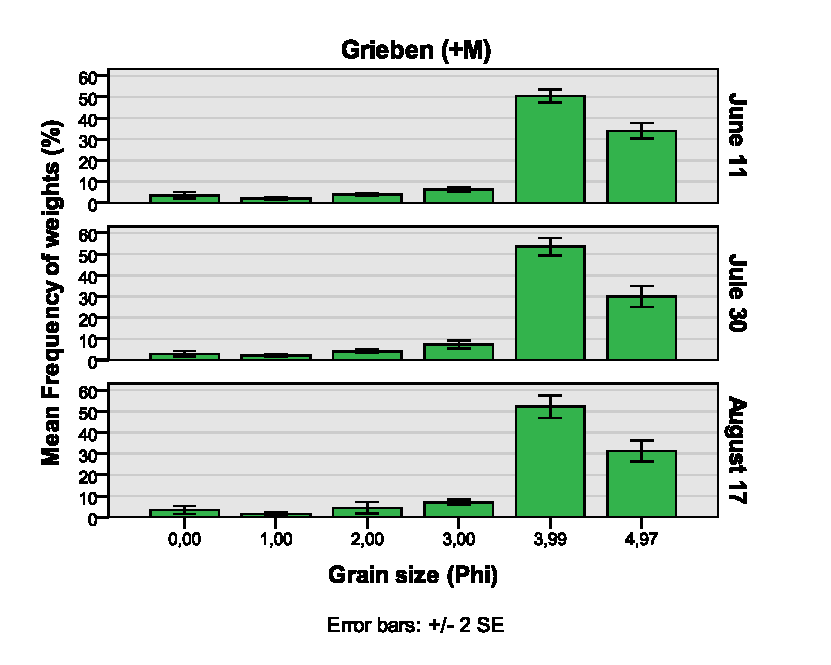
\includegraphics[width=0.70\textwidth]{images/grainsize/sediment_im_jahr3.eps}
\caption[Korngrößenverteilungen Grieben (+M)]{Korngrößenverteilungen am dicht bewachsenen Standort in der Griebener Bucht; Messparallelen aus 5 Sedimentkernen}
\label{fig:korngrössen_Grieben_+m}
\end{figure}




\subsubsection{Grieben, spärlich bewachsener Standort}

Hier ist die Korngrößenverteilung signifikant unterschiedlich gegenüber der der dicht mit Phytobenthos besiedelten Untersuchungsgruppe. Sie ist nur leicht linksschief, fast symmetrisch. Der Median der Korngröße beträgt \unit{3,42-3,47}{$\phi$}, wobei im Juli signifikant geringere Werte gefunden wurden als im Juni und im August. Das bedeutet, dass im Juli der Anteil der feinkörnigeren Fraktionen im Mittel etwas geringer war. Grund hierfür ist ein leichter Anstieg der Feinsandfraktion und ein Rückgang sehr feiner Sande, Tone und Silte. Im Mittel ist das Sediment hier etwas gröber als im dicht besiedelten Bereich der Bucht und der Silt-/ Tonanteil deutlich geringer. Grobsande sind kaum enthalten und das Sediment ist aufgrund der Dominanz der sehr feinen Sandfraktion mit einem Anteil von etwa \unit{60-70}{\%} an der Gesamtprobe mäßig sortiert. Der organische Anteil beträgt \unit{0,1-0,2}{\%} und ist deutlich geringer als am vegetationsdominierten Standort, jedoch mit dem vegetationsarmen Standort des Vitter Bodden vergleichbar.



\begin{figure}[!htb]
\centering
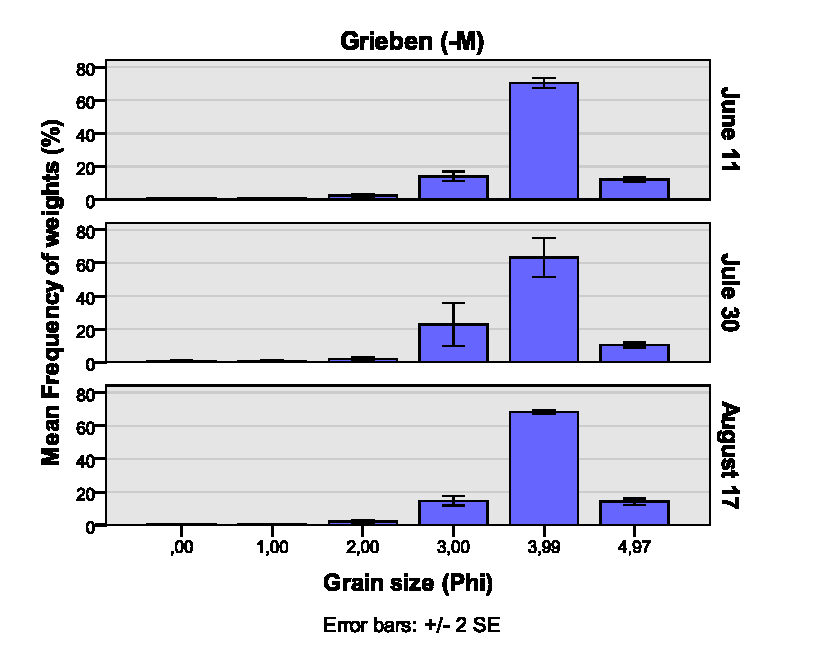
\includegraphics[width=0.70\textwidth]{images/grainsize/sediment_im_jahr4.eps}
\caption[Korngrößenverteilungen Grieben (-M)]{Korngrößenverteilungen am spärlich bewachsenen Standort in der Griebener Bucht; Messparallelen aus 5 Sedimentkernen}
\label{fig:korngrössen_Grieben_-m}
\end{figure}




\FloatBarrier



\begin{figure}[htb]
\centering
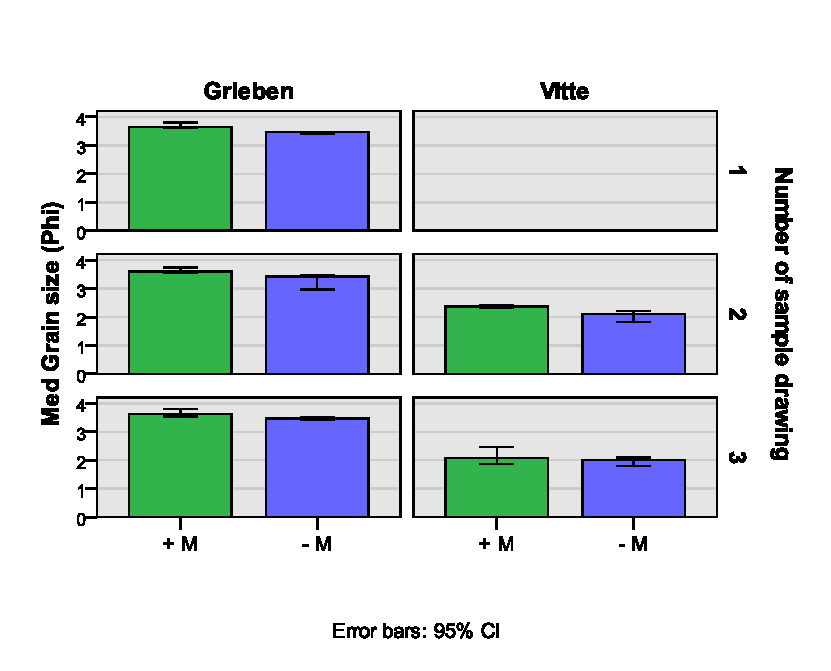
\includegraphics[width=0.70\textwidth]{images/sedimentparameter/S-Parameter_MD_KG_neu1.eps}
\caption[Median der Korngröße Grieben und Vitte]{Median der Korngröße an dicht (+M) und spärlich (-M) bewachsenen Standorten im Vitter Bodden und in der Griebener Bucht im Verlauf der Wachstumsperiode}
\label{fig:md_korngröße}
\end{figure}


\begin{figure}[htb]
\centering
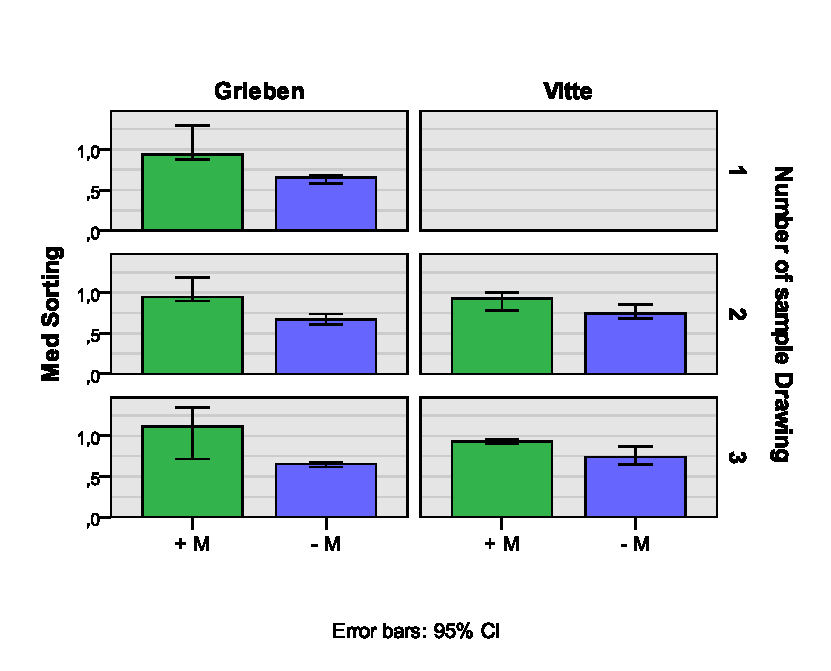
\includegraphics[width=0.70\textwidth]{images/sedimentparameter/S_Parameter_Sortierung_neu1.eps}
\caption[Sortierung der Sedimente in Grieben und Vitte]{Sortierung der Sedimente an dicht (+M) und spärlich (-M) bewachsenen Standorten im Vitter Bodden und in der Griebener Bucht im Verlauf der Wachstumsperiode}
\label{fig:sortierung}
\end{figure}



\begin{figure}[htb]
\centering
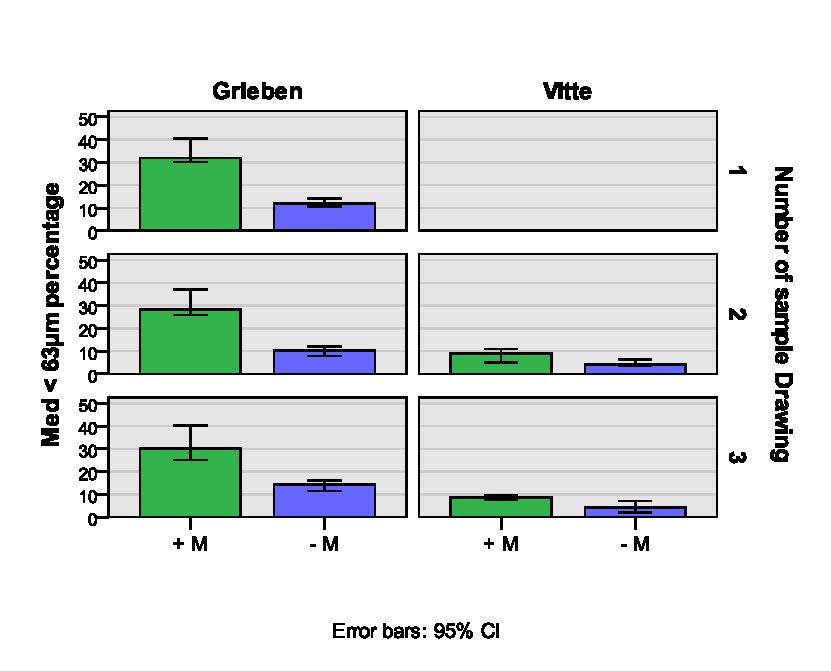
\includegraphics[width=0.70\textwidth]{images/sedimentparameter/S_Parameter_63_neu1.eps}
\caption[Anteil der \unit{<63}{\mu\metre}-Korngrößenfraktion in Grieben und Vitte]Anteil der \unit{<63}{\mu\metre}-Korngrößenfraktion an dicht (+M) und spärlich (-M) bewachsenen Standorten im Vitter Bodden und in der Griebener Bucht im Verlauf der Wachstumsperiode}
\label{fig:63}
\end{figure}


\begin{figure}[htb]
\centering
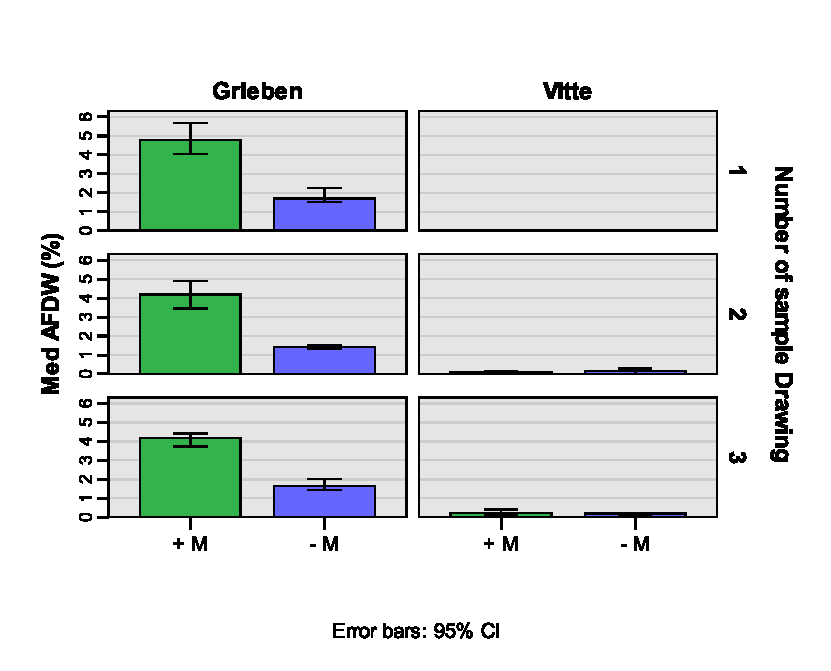
\includegraphics[width=0.70\textwidth]{images/sedimentparameter/afdg_neu1.eps}
\caption[Organischer Gehalt des Sedimentes in Grieben und Vitte]{Organischer Gehalt des Sedimentes, ermittelt als aschfreies Trockengewicht (AFDW) an dicht (+M) und spärlich (-M) bewachsenen Standorten im Vitter Bodden und in der Griebener Bucht im Verlauf der Wachstumsperiode}
\label{fig:afdg_sediment}
\end{figure}

\clearpage

\section{Ergebnisse - Standorte entlang des Salzgradienten}

\subsection{Detaillierte Vegetationsstruktur}

\subsubsection{Geltinger Bucht}

Die Vegetationsbestände in der Geltinger Bucht (dicht bewachsener Standort) setzen sich zusammen aus \textit{Zostera marina} und \textit{Fucus vesiculosus f. balticus}. Das Seegras wuchs bis \unit{30}{\centi\metre} vom Grund mit Deckungsgraden von \unit{70-80}{\%}. In den Wasserschichten \unit{30 bis 60}{\centi\metre} über dem Grund reduzierte sich die Deckung allmählich bis auf \unit{10}{\%}. Nur wenige der schmalen Blattspreiten erstreckten sich darüber hinaus bis zur Oberfläche. Das Wasser war hier etwa \unit{100}{\centi\metre} tief.

Der lose Blasentang ist von kräftigem Wuchs und bedeckt den Boden mit \unit{20}{\%}. Auf \unit{20 und 30}{\centi\metre} Höhe gehen die Pflanzen in die Breite und sorgen für Deckungen von \unit{30}{\%}, darüber verschmälert sich der Blasentang wieder. Große Exemplare erreichten Wuchshöhen von bis zu \unit{50}{\centi\metre}.
In der Mitte der Wassersäule befanden sich mit Deckungsgraden unter einem Prozent freischwimmende filamentöse Algen, die jedoch an zwei Plots Deckungen von \unit{10 und 20}{\%} ausmachten. Die Gesamtdeckung auf den Flächen betrug \unit{90}{\%}, diese wurden vom Grund bis \unit{20}{\centi\metre} Wuchshöhe kartiert, danach nahmen die Deckungen stetig bis zur Oberfläche ab.

\subsubsection{Orther Bucht}

Die Orther Bucht ist zu \unit{30-60}{\%}, im Mittel mit \unit{40}{\%} mit Pflanzen bedeckt. Auf \unit{10}{\centi\metre} Entfernung vom Grund sind \unit{30}{\%} der Wasserschicht bedeckt, darüber ragen nur noch einzelne Stängel von \textit{Potamogeton pectinatus} bis \unit{40}{\centi\metre} Höhe. Das Wasser an diesem Standort ist im Mittel \unit{70}{\centi\metre} tief. Bestandsbildende Art ist \textit{Zannichellia palustris} mit Deckungen von \unit{20-40}{\%}. An einem Plot fehlte die Art, dafür kam hier \textit{Ruppia cirrhosa} mit einer Deckung von \unit{40}{\%} vor. Ebenfalls deckten filamentöse Algen auf \unit{5 bis 10}{\centi\metre} Wuchshöhe zu \unit{20}{\%} den Standort ab. \textit{Potamogeton pectinatus} kam mit Deckungen von bis zu \unit{10}{\%} am Grund vor und verschmälerte sich in der Wassersäule. Von \textit{Chara canescens} und \textit{Tolypella nidifica} wurden vereinzelt Exemplare gefunden.

\subsubsection{Salzhaff}

Das Salzhaff ist zu \unit{80-90}{\%} mit Vegetation bedeckt. Davon machen nicht fest verankerte, filamentöse Algen mit \unit{80}{\%} Deckung auf \unit{5}{\centi\metre} Wuchshöhe den größten Anteil aus. Ihr Anteil reduziert sich in der Wassersäule allmählich bis auf \unit{50}{\centi\metre} Wuchshöhe. \textit{Potamogeton pectinatus} ist mit \unit{30-60}{\%} Deckung die bastandsbildene festsitzende Pflanzenart. Auch sein Anteil reduziert sich allmählich bis \unit{50}{\centi\metre} Wuchshöhe, darüber hinaus reichen wenige Äste bis zur Oberfläche. Das Wasser an diesem Standort ist \unit{80 bis 90}{\centi\metre} tief. Vereinzelt kam auch \textit{Zannichellia palustris} und lose am Grund die Grünalge \textit{Monostroma sp.} vor.

\subsubsection{Spandowerhagener Wiek}

Die gesamte Spandowerhagener Wiek war zu etwa \unit{90}{\%} mit Pflanzen bedeckt, es gab keine ausgedehnten freien Flächen. Den Hauptanteil der Vegetation bildete \textit{Potamogeton pectinatus} mit Deckungsgraden von im Mittel \unit{90}{\%} am Grund, sich allmählich in der Wassersäule reduzierend. Dabei trägt er auf \unit{30}{\centi\metre} Wuchshöhe noch zu einer mittleren Deckung von \unit{50}{\%} bei und wächst bis \unit{50}{\centi\metre} auf. Das Wasser ist \unit{80-85}{\centi\metre} tief. Außerdem kommen \textit{Myriophyllum spicatum} mit \unit{10 bis 20}{\%} Deckung und \textit{Potamogeton perfoliatus}, auf einigen Plots mit bis zu \unit{10}{\%} Deckung vor. \textit{Myriophyllum spicatum} bedeckt mit einem Grund-Abstand von \unit{10 und 20}{\centi\metre} noch \unit{10 bzw. 5}{\%} der jeweiligen Wasserschichten, nur vereinzelte Halme wachsen bis \unit{50}{\centi\metre} auf. \textit{Potamogeton perfoliatus} hingegen nimmt nur bis auf \unit{10}{\centi\metre} relevante Deckungen ein, darüber hinaus gehen wenige Zweige bis \unit{70}{\centi\metre} Wuchshöhe. Auf 2 Plots wurde auch mit \unit{10 bzw. 20}{\%} Anteil in der \unit{5 bis 10}{\centi\metre} -Wasserschicht \textit{Zannichellia palustris} gefunden und es gab wenige vereinzelte Exemplare von \textit{Najas marina}.





\begin{figure}[!htb]
\centering
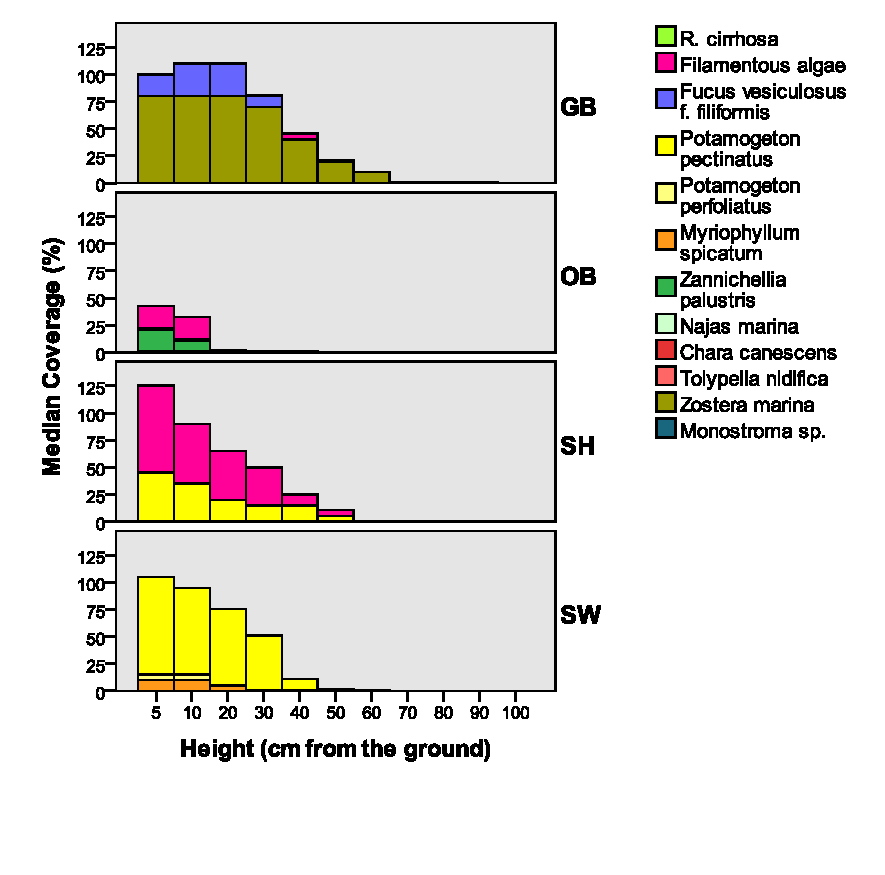
\includegraphics[0.90\textwidth]{images/Wuchshoehenkartierung/salzgradient_gross1.eps}
\caption[Höhenstufenkartierung an den Stationen des Salzgradienten (+M)]{Deckungen aller Arten auf Höhenstufen vom Grund bis zur Oberfläche an den dicht bewachsenen Standorten entlang des Salzgradienten; GB = Geltinger Bucht, OB = Orther Bucht; SH = Salzhaff; SW = Spandowerhagener Wiek}
\label{fig:wuchshoehen_salzgradient_1}
\end{figure}
\\
\begin{figure}[!htb]
\centering
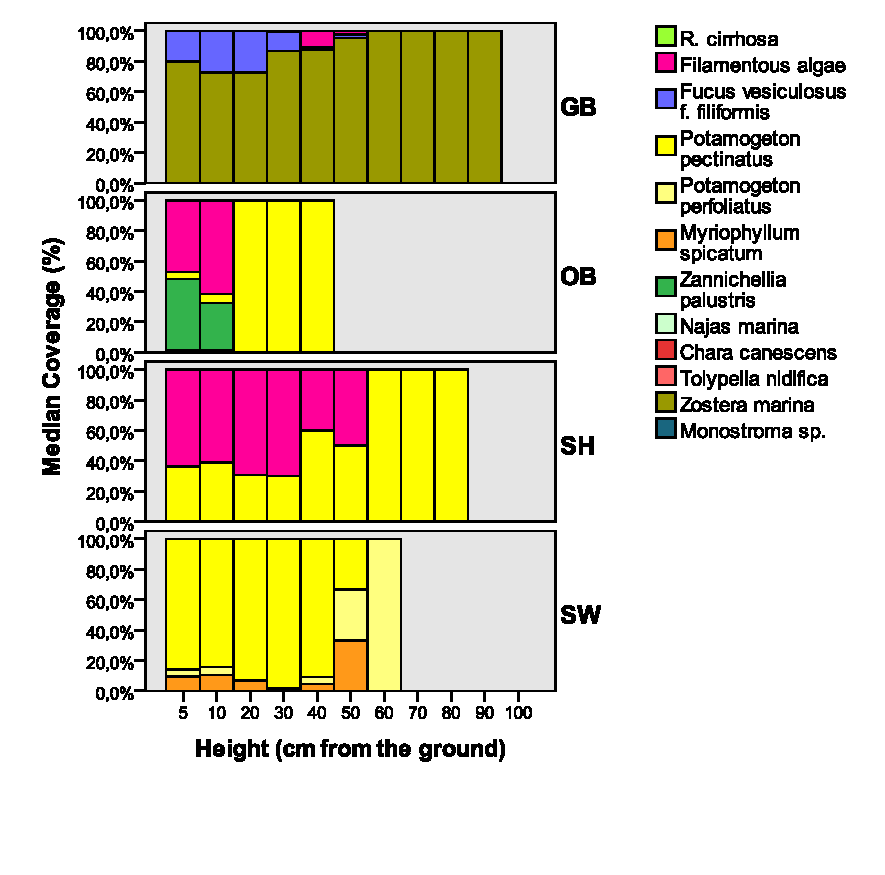
\includegraphics[0.90\textwidth]{images/Wuchshoehenkartierung/salzgradient_gross2.eps}
\caption[Prozentuale Höhenstufenkartierung an den Stationen des Salzgradienten (+M)]{Prozentuale Deckungen aller Arten, bezogen auf die Gesamtdeckung auf jeder Höhenstufe an den dicht bewachsenen Standorten entlang des Salzgradienten; GB = Geltinger Bucht, OB = Orther Bucht; SH = Salzhaff; SW = Spandowerhagener Wiek}
\label{fig:wuchshoehen_salzgradient_2}
\end{figure}

\FloatBarrier


\subsection{Deckung und PVI}

Zum Zeitpunkt der Probenahmen entlang des Salzgradienten waren sowohl die Deckung als auch das PVI an allen vegetationsarmen Untersuchungsgruppen sehr gering. Maximal \unit{2}{\%} der Fläche wurden von Phytobenthos eingenommen und es machte maximal \unit{0,3}{\%} der Wassersäulen aus.

Bei Betrachtung aller vegetationsdominierten Stationen des Salzgradienten im Vergleich zeigt sich, dass es 3 verschiedene Kategorien von Vegetationsbeständen gab. In die erste Kategorie fallen die Orther Bucht und die Griebener Bucht. Diese zeigten Deckungsgrade von \unit{40-60}{\%}. Auch ihre pflanzliche Zusammensetzung ist sich ähnlich. Es gibt grundrasenbildende Arten (\textit{Zannichellia palustris} in der Orther Bucht und\textit{ Ruppia cirrhosa} in der Griebener Bucht) sowie das höher aufwachsende Laichkraut \textit{Potamogeton pectintus} und dazwischen Matten aus fädigen Algen. In dem verhältnismäßig flachen Wasser von \unit{60-70}{\centi\metre} werden PVI-Werte von im Mittel \unit{5}{\%} erreicht. Das Maximum waren \unit{14,4}{\%} in der Orther Bucht.

Die Geltinger Bucht, das Salzhaff und die Spandowerhagener Wiek bilden die zweite Kategorie mit wesentlich höheren Deckungsgraden von \unit{80-95}{\%} und ebenfalls hohen PVI-Werten von \unit{20-30}{\%}. Diese Standorte befinden sich auch in etwas tieferem Wasser (\unit{80-110}{\centi\metre}). Die Geltinger Bucht und die Spandowerhagener Wiek sind sich auch in ihrer Vegetationsstruktur ähnlich. Beide beherbergen Makrophyten, die weit in die Wassersäule hineinreichen und auch in größerem Abstand vom Grund noch hohe Deckungsgrade verursachen. In der Geltinger Bucht ist dies \textit{Zostera marina} und in der Spandowerhagener Wiek sind es Parvopotamiden und \textit{Myriophyllum spicatum}. Im Salzhhaff hingegen werden die hohen Deckungsgrade und pflanzlichen Anteile in der Wassersäule neben dem hoch aufwachsenden \textit{Potamogeton pectintus} zu einem großen Teil von filamentösen Algen verursacht.

Die dritte Kategorie nimmt der Vitter Bodden ein. Bei einer Bedeckung von \unit{100}{\%} ist der Anteil des Phytobenthos an der Wassersäule mit \unit{8-17}{\%} deutlich weniger als bei den 3 zuvor genannten Standorten. Grund hierfür ist die dichte Bedeckung mit \textit{Fucus vesiculosus}, welcher zwar hohe Deckungsgrade verursacht, aber nicht weit in die etwa \unit{83}{\centi\metre} tiefe Wassersäule hineinreicht.



\begin{figure}[!htb]
\centering
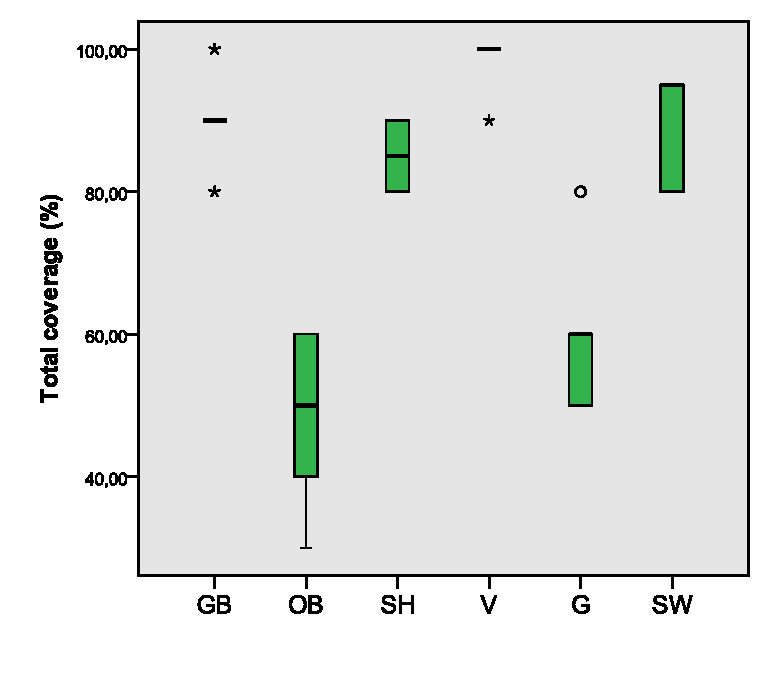
\includegraphics[width=0.80\textwidth]{images/total_cover/cover_salzgradient.eps}
\caption[Bedeckung mit Makrophyten an Standorten entlang des Salzgradienten]{Gesamtbedeckung der Plots mit Makrophyten an den dicht bewachsenen Standorten entlang des Salzgradienten; GB = Geltinger Bucht, OB = Orther Bucht; SH = Salzhaff; SW = Spandowerhagener Wiek}
\label{fig:cover_salzgradient}
\end{figure}

\begin{figure}[!htb]
\centering
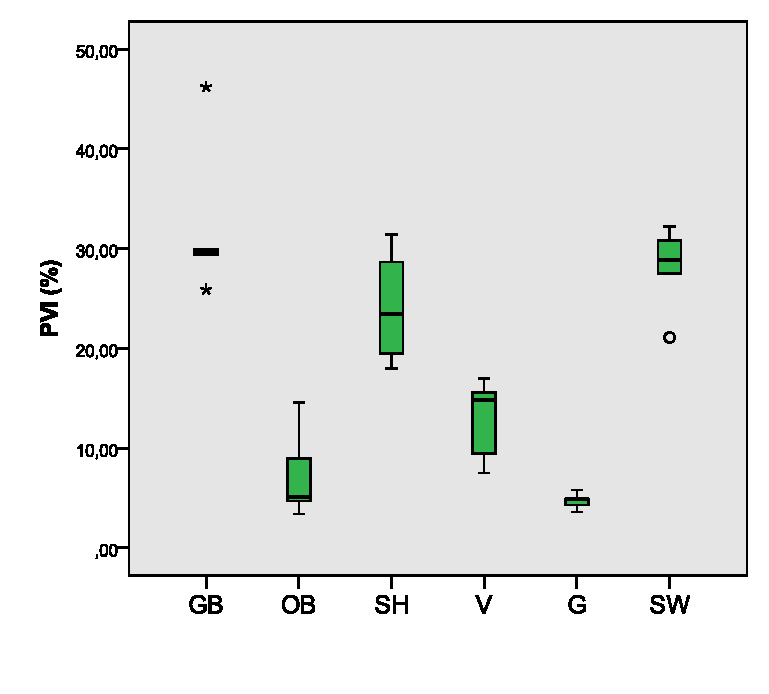
\includegraphics[width=0.80\textwidth]{images/pvi/pvi_salzgradient.eps}
\caption[PVI an Standorten entlang des Salzgradienten]{Anteil des Phytobenthos an der Wassersäule (PVI nach \cite{jeppesen_1998}) an den dicht bewachsenen Standorten entlang des Salzgradienten; GB = Geltinger Bucht, OB = Orther Bucht; SH = Salzhaff; SW = Spandowerhagener Wiek}
\label{fig:pvi_salzgradient}
\end{figure}



\begin{table}[!htb]
\centering
\caption[Deskriptive Statistik, Deckung und PVI entlang des Salzgradienten]{Deskriptive Statistik zu Deckung und PVI an Standorten entlang des Salzgradienten; MAD = Mittlere Abweichung vom Median}
\begin{tabular}{llllll}
\toprule
Category & Location 							& \multicolumn{2}{l}{Total Cover} & \multicolumn{2}{l}{PVI}\\
		 &											& Median	& MAD			  & Median	& MAD\\
\midrule
\multirow{6}{*}{Dense Vegetation}& Geltinger Bucht	& 90.00		& 4.00			  & 29.60	& 4.16\\
								 & Orther Bucht		& 50.00		& 10.00			  & 5.10	& 3.10\\
								 & Salzhaff			& 85.00		& 5.00			  & 23.35	& 4.58\\
								 & Vitter Bodden	& 100.00	& 2.00			  & 14.80	& 3.12\\
								 & Griebener Bucht	& 60.00		& 8.00			  & 4.90	& 0.56\\
								 & Spandowerhagener Wiek & 95.00 & 6.00			  & 28.90	& 2.88\\
\midrule
\multirow{5}{*}{Sparse Vegetation}&Geltinger Bucht	& 2.00		& 0.00			  & 0.18	& 0.00\\
								 & Orther Bucht		& 2.00		& 				  & 0.30\\
								 & Salzhaff			& 0.50		& 0.00			  & 0.10	& 0.00\\
								 & Vitter Bodden	& 0.50		& 0.00			  & 0.00	& 0.00\\
								 & Griebener Bucht	& 2.50		& 1.30			  & 0.33	& 0.01\\
\bottomrule
\end{tabular}
\label{tab:statistik_salzgradient_Deckung,PVI}
\end{table}
\FloatBarrier



\subsection{Sediment}

\subsubsection{Geltinger Bucht}

Das Sediment am dicht mit Phytobenthos besiedelten Standort ist mäßig sortiert und die Verteilungskurve etwas in den grobkörnigen Bereich verschoben. Feinsand und Mittelsand haben mit \unit{45 und 27,5}{\%} den größten Anteil am Gesamt-Korngrößenspektrum. Mit \unit{9 und 8,3}{\%} sind auch sehr grobe und grobe Sande im Sediment enthalten und mit je etwa \unit{5}{\%} sind Feinsand und Ton-/Siltfraktionen vertreten. Der Median der Korngrößenverteilung beträgt $ \Phi $ = 2,1 und der organische Gehalt \unit{1,4}{\%}.

Das Sediment der kaum mit Phytobenthos besiedelten Untersuchungsgruppe war besser sortiert als die der dicht besiedelten Gruppe. Feinsande und Mittelsande hatten hier einen größeren Anteil von \unit{53 und 34}{\%}. Sehr grober Sand war fast nicht und grober Sand nur zu \unit{3}{\%} enthalten. Es waren weniger feine Sande (\unit{2,5}{\%}) aber dafür mit etwa \unit{7}{\%} mehr Ton und Silt enthalten. Der Organische Gehalt ist mit \unit{0,7}{\%} geringer als bei den Sedimenten der dicht mit Seegras und \textit{Fucus vesiculosus} besiedelten Fläche.



\subsubsection{Orther Bucht}

Auf der Phytobenthos-dominierten Untersuchungsfläche ist das Sediment sehr gut sortiert und die Feinsandfraktion dominiert mit \unit{72}{\%}. Daneben kommen zu \unit{16 und 7}{\%} sehr feine und Mittelsande vor. Der Anteil der \unit{<63}{\mu\metre}-Fraktion beträgt hier nur \unit{3}{\%}. Insgesamt ist die Verteilungskurve leicht linksschief (in den feinkörnigen Bereich verschoben) und der Median der Korngröße beträgt $ \Phi $ = 2,6. Der organische Gehalt des Sedimentes ist mit \unit{0,5}{\%} sehr gering.

Das Sediment der vegetationsreichen Untersuchungsgruppe hingegen ist weniger gut sortiert. Mit \unit{62}{\%} ist der Feinsand ebenfalls die am meißten vertretene Korngrößenfraktion, jedoch ist auch der Anteil des Mittelsandes mit etwa \unit{18}{\%} höher. Der Median der Korngröße beträgt $ \Phi $ = 2,5. 

\subsubsection{Salzhaff}

Hier sind sich die Korngrößenfraktionen der dicht und spärlich besiedelten Untersuchungsflächen ähnlich. Die Sedimente sind gut sortiert. Mit \unit{63,5}{\%} (vegetationsarme Gruppe) bzw. \unit{72}{\%} (vegetationsreiche Gruppe) dominieren sehr feine Sande. Daneben kommen Silte und Tone mit \unit{10 bis 12}{\%} sowie Feinsande mit  \unit{15-25}{\%} vor. Im wenig besiedelten Bereich ist der Anteil der Silte und Tone geringer und der Anteil der Feinsande deutlich höher als im dicht besiedelten Bereich. Mittel-bis Grobsande haben keine Bedeutung in den  Korngrößenverteilungen beider Gruppen. Der Median der Korngröße ist in der dicht besiedelten Gruppe mit $ \Phi $ = 3,5 etwas höher als der der spärlich besiedelten Gruppe ($ \Phi $ = 3,4). Das bedeutet, dass Sediment ist in der dicht besiedelten Gruppe etwas feiner. Der organische Gehalt der Sedimente beträgt \unit{1,2 und 0,8}{\%}. Er ist in der dicht besiedelten Untersuchungsgruppe etwas höher. 


\subsubsection{Spandowerhagener Wiek}

In der durchgängig von dichter Vegetation geprägten Spandowerhagener Wiek war das Sediment gut sortiert und die Korngrößenverteilung annähernd symmetrisch. Mit \unit{72,5}{\%} dominiert der Anteil der Feinsandfraktion. 
Daneben haben Mittelsande, sehr feine Sande und Silte / Tone mit \unit{17}{\%}, \unit{6}{\%}, und \unit{3}{\%} ihre jeweiligen Anteile am Sediment. Der Median der Korngrößenverteilung liegt bei $ \Phi $ = 2,4 und der organische Gehalt beträgt \unit{0,9}{\%}.

\begin{table}[!htb]
\centering
\caption[Deskriptive Statistik zu den Korngrößenverteilungen entlang des Salzgradienten]{Deskriptive Statistik zu den Korngrößenverteilungen an den Standorten entlang des Salzgradienten; MAD = Mittlere Abweichung vom Median; +M = dichte Vegetation, -M = spärliche Vegetation; Kennwerte aus den obersten \unit{2}{\centi\metre} des Sedimentkörpers}
\begin{tabular}{lcrrrr}

\toprule

\multicolumn{1}{c}{Location}  & \multicolumn{1}{c}{Category} & \multicolumn{1}{c}{Med Grain Size} & \multicolumn{1}{c}{Sorting} & \multicolumn{1}{c}{< \unit{63}{\mu\metre}} & \multicolumn{1}{c}{AFDW}\\

& 	& \multicolumn{1}{c}{$ (\Phi) $} & & \multicolumn{1}{c}{(\%)} & \multicolumn{1}{c}{(\% DW)}\\

\midrule
\multirow{2}{*}{Geltinger Bucht} & +M & 2.12 & 0.71 & 4.94 & 1.42\\
								 & -M & 2.24 & 0.54 & 6.88 & 0.72\\
\midrule
\multirow{2}{*}{Orther Bucht} & +M  & 2.57 & 0.35 & 3.03 & 0.52\\
							& -M  & 2.46 & 0.41 & 4.00 & 0.55\\
\midrule
\multirow{2}{*}{Salzhaff} & +M & 3.47 & 0.35 & 12.15 & 1.21\\
						& -M & 3.37 & 0.40 & 10.45 & 0.78\\
\midrule
\multirow{2}{*}{Vitter Bodden} & +M & 2.23 & 0.54 & 6.04 & 1.23\\
								& -M & 1.89 & 0.56 & 5.56 & 0.91\\
\midrule
\multirow{2}{*}{Griebener Bucht} & +M & 3.61 & 0.95 & 28.31 & 4.19\\
								& -M & 3.42 & 0.67 & 10.23 & 1.43\\
\midrule
\multirow{1}{*}{Spandowerhagener Wiek} & +M & 2.44 & 0.36 & 2.84 & 0.93\\
\bottomrule

\end{tabular}
\label{tab:statistik_salzgradient_sedimentparameter}
\end{table}
\\


\begin{figure}[!htb]
\centering
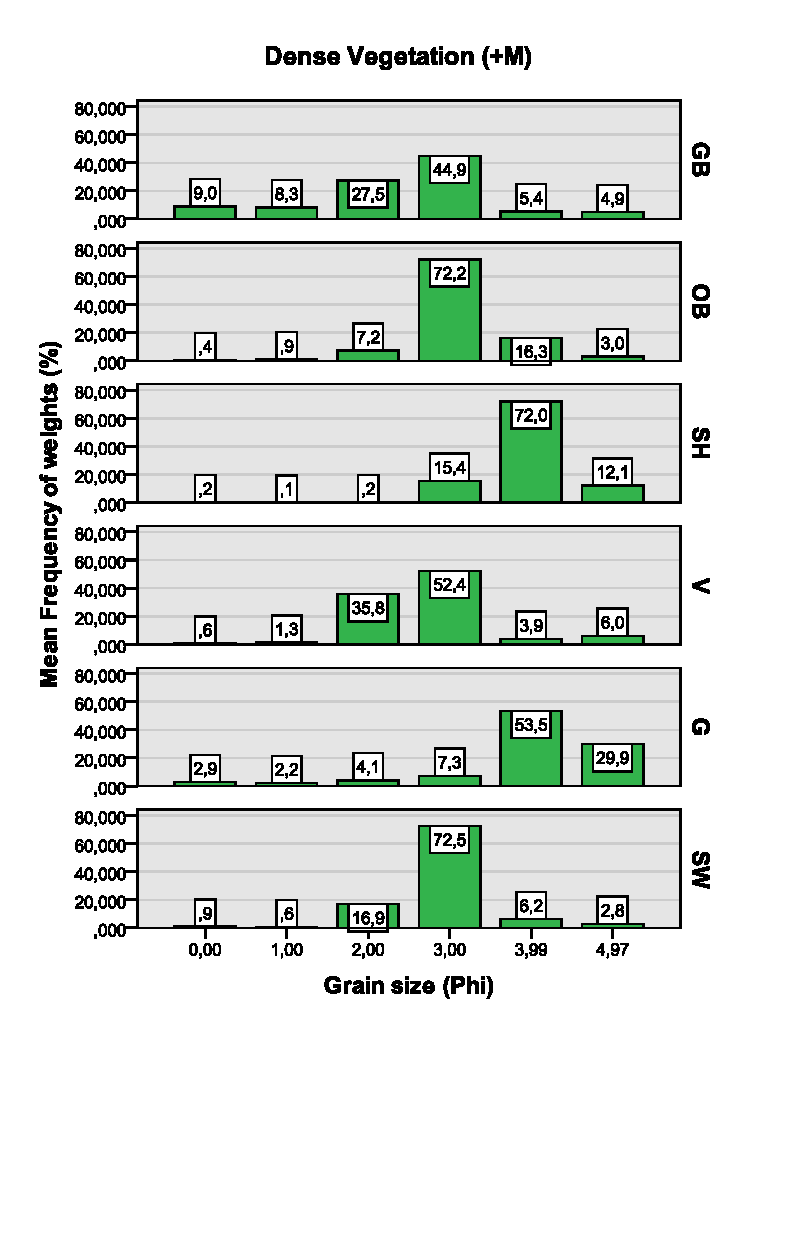
\includegraphics[trim = 0mm 35mm 0mm 0mm, clip, width=0.90\textwidth]{images/grainsize/korngroessenverteilungen_sg1.eps}
\caption[Korngrößenverteilungen entlang des Salzgradienten (+M)]{Korngrößenverteilungen an dicht bewachsenen Standorten entlang des Salzgradienten (+M); GB = Geltinger Bucht, OB = Orther Bucht; SH = Salzhaff; V = Vitter Bodden (5.7.2013), G = Griebener Bucht (30.7.2013), SW = Spandowerhagener Wiek}
\label{fig:korngrössen_salzgradient_+m}
\end{figure}

\begin{figure}[!htb]
\centering
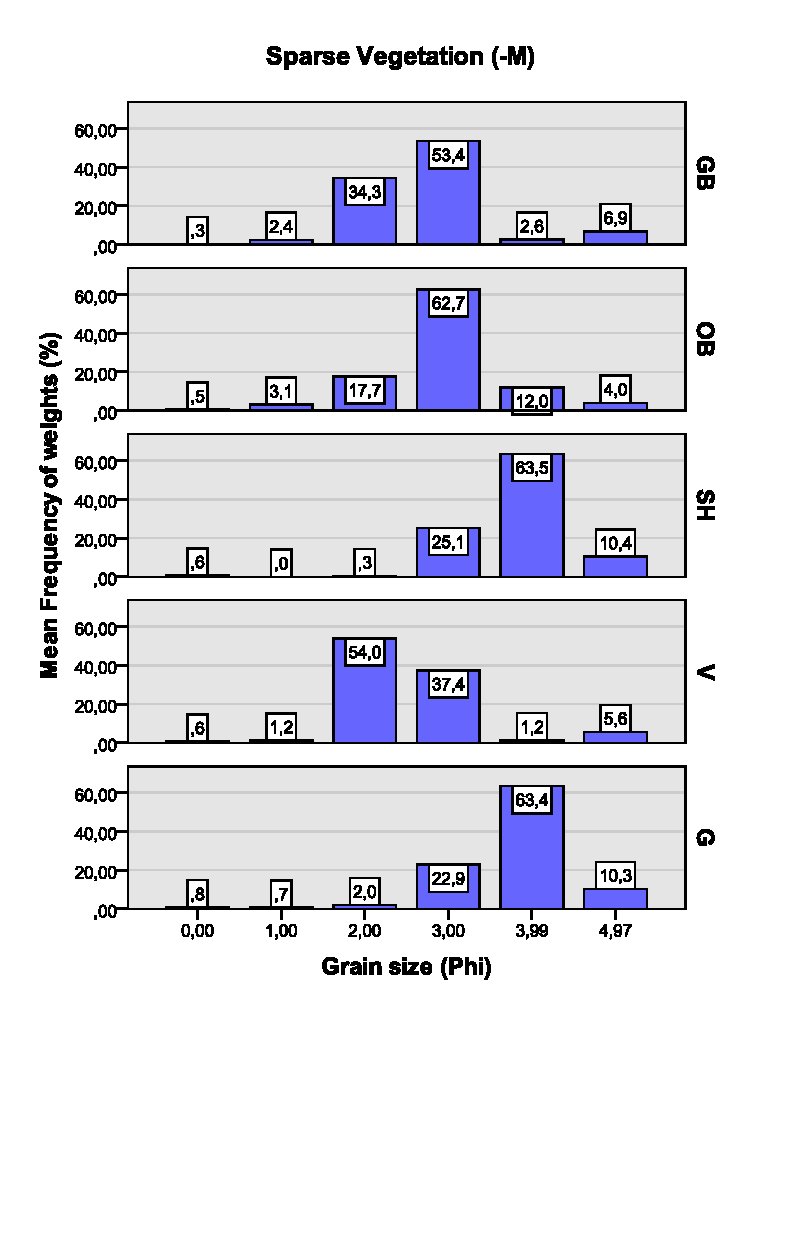
\includegraphics[trim = 0mm 35mm 0mm 0mm, clip, width=0.90\textwidth]{images/grainsize/korngroessenverteilungen_sg2.eps}
\caption[Korngrößenverteilungen entlang des Salzgradienten (-M)]{Korngrößenverteilungen an spärlich bewachsenen Standorten entlang des Salzgradienten (-M); GB = Geltinger Bucht, OB = Orther Bucht; SH = Salzhaff; V = Vitter Bodden (5.7.2013), G = Griebener Bucht (30.7.2013), SW = Spandowerhagener Wiek}
\label{fig:korngrössen_salzgradient_-m}
\end{figure}

\begin{figure}[!htb]
\centering
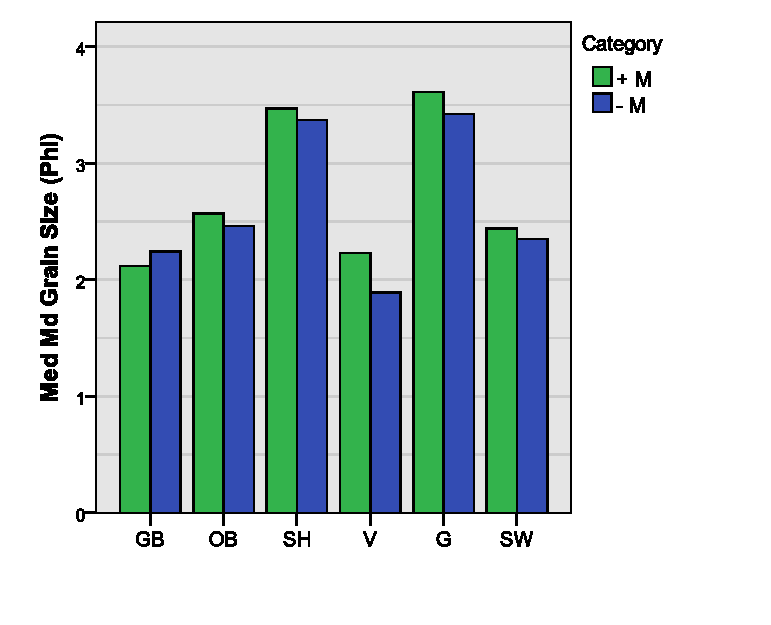
\includegraphics[width=0.75\textwidth]{images/salzsedimentauswertung/bar_mgsize.eps}
\caption[Median der Korngrößen an Stationen des Salzgradienten]{Median der Korngrößen an Stationen des Salzgradienten; GB = Geltinger Bucht, OB = Orther Bucht; SH = Salzhaff; V = Vitter Bodden (5.7.2013), G = Griebener Bucht (30.7.2013), SW = Spandowerhagener Wiek}
\label{fig:sg:mittlere_kg}
\end{figure}

\begin{figure}[!htb]
\centering
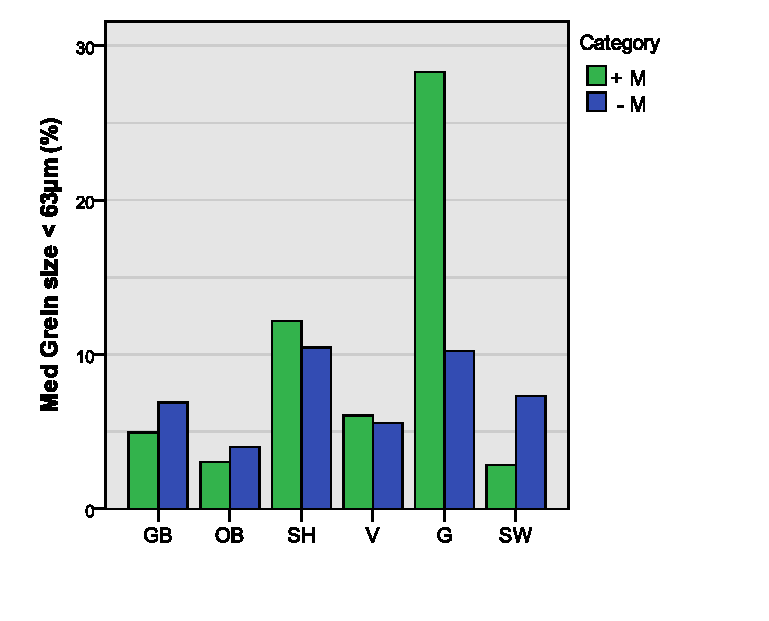
\includegraphics[width=0.75\textwidth]{images/salzsedimentauswertung/bar_63.eps}
\caption[Anteil der \unit{<63}{\mu\metre}-Korngrößenfraktion an Stationen des Salzgradienten]{Anteil der \unit{<63}{\mu\metre}-Korngrößenfraktion an Stationen des Salzgradienten; GB = Geltinger Bucht, OB = Orther Bucht; SH = Salzhaff; V = Vitter Bodden (5.7.2013), G = Griebener Bucht (30.7.2013), SW = Spandowerhagener Wiek}
\label{fig:sg:kleiner_63}
\end{figure}

\begin{figure}[htb]
\centering
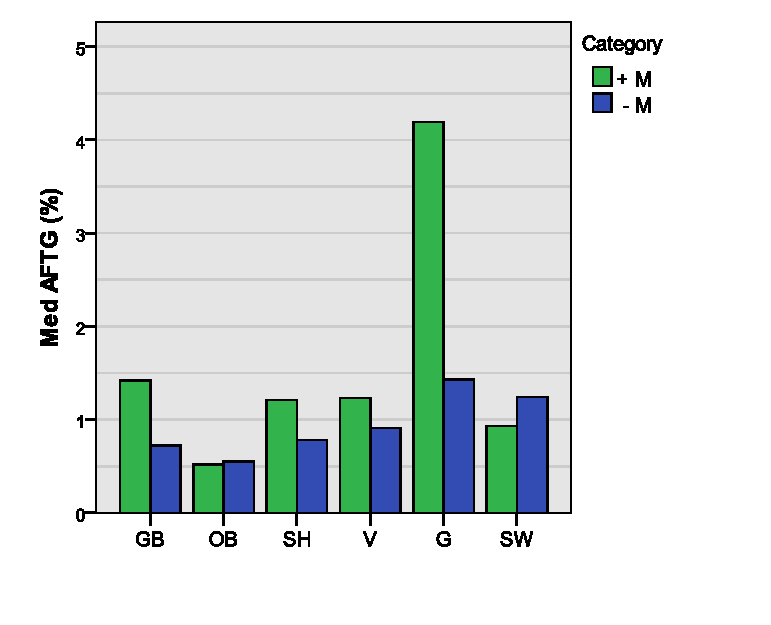
\includegraphics[width=0.75\textwidth]{images/salzsedimentauswertung/bar_aftg.eps}
\caption[Organischer Gehalt der Sedimente an Stationen des Salzgradienten]{Organischer Gehalt der Sedimente  an Stationen des Salzgradienten; GB = Geltinger Bucht, OB = Orther Bucht; SH = Salzhaff; V = Vitter Bodden (5.7.2013), G = Griebener Bucht (30.7.2013), SW = Spandowerhagener Wiek}
\label{fig:sg:afdg}
\end{figure}
\FloatBarrier

\subsubsection{Zusammenhänge zwischen Vegetation und Korngrößen}

Im Vergleich der Vegetation (Deckung und PVI) mit dem Median der Korngröße aller Standorte entlang des Salzgradienten ergibt sich keine lineare Abhängigkeit zwischen den Parametern (vgl. Abbildung \ref{fig: Regression_Vegetation_Korngroesse}). Das heißt es gibt keine tendenzielle Abnahme der Korngröße bei zunehmenden Deckungsgraden oder Anteilen der Vegetation an der Wassersäule. 

Werden alle Stationen einzeln betrachtet, fällt auf, dass der Median der Korngrößen, mit Ausnahme der Geltinger Bucht, an den spärlich bewachsenen Stellen um 0,1 bis 0,34 $ \Phi$-Einheiten niedriger, das Sediment also etwas grobkörniger ist (Vgl. Abbildung \ref{fig:sg:mittlere_kg}).

Auch beim Vergleich der feinsten Siebfraktion (\unit{<63}{\mu\metre}) mit den Vegetationsparametern Deckung und PVI ergibt sich keine lineare Beziehung (Vgl. Abbildung \ref{fig: Regression_Vegetation_63}). Im Vergleich zwischen dicht und spärlich besiedelten Untersuchungsgruppen ist ebenfalls kein Hinweis darauf zu finden, dass  es einen Zusammenhang zwischen dem Bewuchs mit Phytobenthos und dem Anteil der Ton/Siltfraktion gäbe. 



\begin{figure}[htb]
        \centering
        \begin{subfigure}[htb]{0.45\textwidth}
                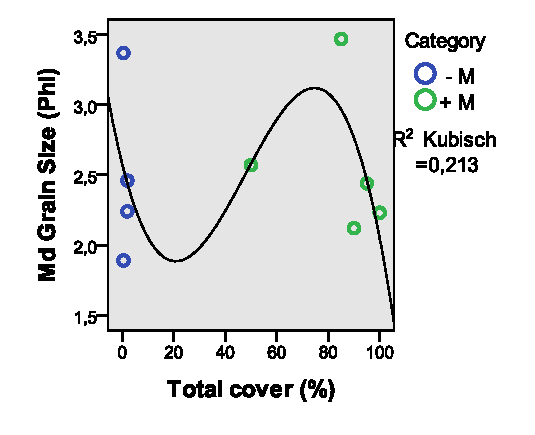
\includegraphics[width=\textwidth]{images/salzsedimentauswertung/gz_vs_cover.eps}
        \end{subfigure}
        \begin{subfigure}[htb]{0.45\textwidth}
                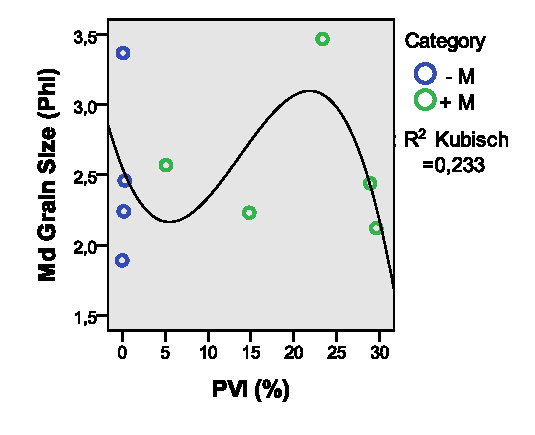
\includegraphics[width=\textwidth]{images/salzsedimentauswertung/gz_vs_pvi.eps}
        \end{subfigure}
        \caption[Regressionsmodell: Vegetation und Median der Korngröße für Stationen des Salzgradienten]												{Zusammenhang zwischen Median der Korngröße und den 																vegetationsbeschreibenden Parametern Deckung (links) und PVI (rechts) für 											Standorte entlang des Salzgradienten}
        \label{fig: Regression_Vegetation_Korngroesse}
\end{figure}

\begin{figure}[!htb]
        \centering
        \begin{subfigure}[htb]{0.45\textwidth}
                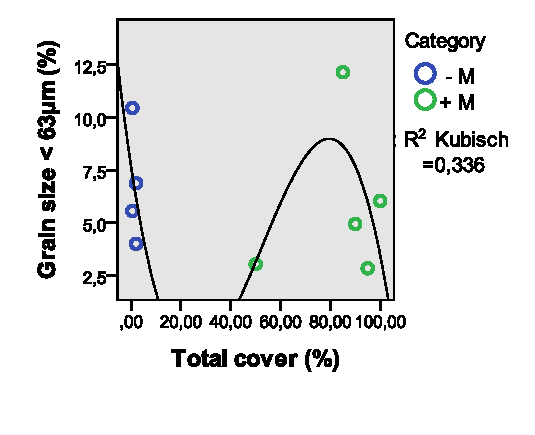
\includegraphics[width=\textwidth]{images/salzsedimentauswertung/63_vs_cover.eps}
        \end{subfigure}
        \begin{subfigure}[htb]{0.45\textwidth}
                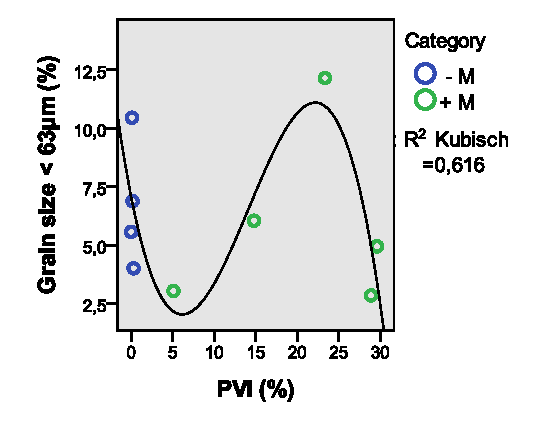
\includegraphics[width=\textwidth]{images/salzsedimentauswertung/63_vs_pvi.eps}
        \end{subfigure}
        \caption[Regressionsmodell: Vegetation und \unit{<63}{\mu\metre}-Korngrößenanteil für Stationen des 											Salzgradienten]{Zusammenhang zwischen \unit{<63}{\mu\metre}-Korngrößenanteil 									und den vegetationsbeschreibenden Parametern Deckung (links) und PVI 												(rechts) für Standorte entlang des Salzgradienten}
        \label{fig: Regression_Vegetation_63}
\end{figure}

\FloatBarrier

In Abbildung \ref{fig:matrixplot} sind verschiedene Parameter bzw. Prädikatoren (Salinität, Wassertiefe, Fetch, Cover, PVI) eingezeichnet, die einen Einfluss auf die mittlere Korngröße haben könnten. Es lässt sich bereits erkennen, dass keine der untersuchten Prädikatoren eine starke lineare Abhängigkeit zur mittleren Korngröße aufweist. Die Windlauflänge (Fetch) sowie die Salinität zeigen in einer Spearman-Rang-Korrelation die größten Abhängigkeiten mit Koeffizienten von -0,6 und 0,6, jedoch mit Irrtumswahrscheinlichkeiten von \unit{7-15}{\%}, dass heißt, diese Parameter könnten die mittlere Korngröße, im Gegensatz zu den Vegetationsparametern beeinflussen, jedoch reichen sie nicht aus, um das Vorhandensein bestimmter mittlerer Korngrößen zu erklären.


\begin{figure}[!htb]
\centering
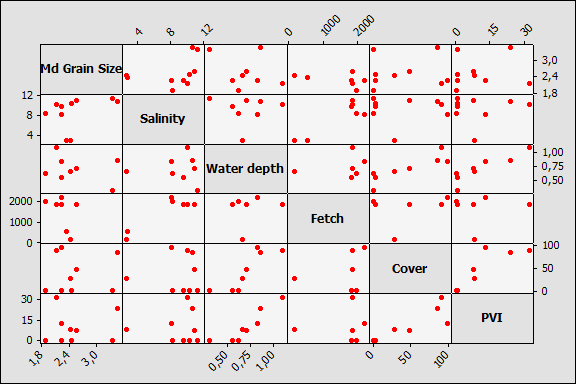
\includegraphics[width=0.75\textwidth]{images/matrixplot/Matrixplot_ohne_Grieben_neu2.png}
\caption[Korrelationsmatrix: Median der Korngröße und 5 Prädikatoren]{Korrelationsmatrix: Median der Korngröße und 5 Prädikatoren: Salinität, Wassertiefe, Fetch, Bedeckung mit Phytobenths und PVI}
\label{fig:matrixplot}
\end{figure}

\FloatBarrier


\begin{table}[!htb]
\centering
\caption[Spearman Rang-Korrelationen zur mittleren Korngröße entlang des Salzgradienten]{Spearman Rang-Korrelationen zur mittleren Korngröße entlang des Salzgradienten; 5 Prädikatoren: Salinität, Wassertiefe, Fetch, Bedeckung mit Phytobenthos, PVI}
\begin{tabular}{lrrrrr}

\toprule
& \multicolumn{5}{c}{Correlation / \textit{p}-Value} \\
\midrule
& \multicolumn{1}{c}{Md Grain Size}  & \multicolumn{1}{c}{Salinity} & \multicolumn{1}{c}{Water Depth} & \multicolumn{1}{c}{Fetch} & \multicolumn{1}{c}{Cover} \\

\midrule

Salinity        &       0,600\\
                &       0,067\\
\midrule
Water depth	    &     	-0,095           &-0,075\\
                &     	0,823            &0,860\\
\midrule
Fetch  	        &   	-0,608           &0,315            &0,371 \\
                &   	0,147            &0,491            &0,468 \\
\midrule
Cover  	        &     	-0,079           &-0,188           &0,888 		&0,282\\
                &     	0,840            &0,628            &0,003 		&0,589\\
\midrule
PVI	            &     	0,057            &-0,124           &0,915			&0,022            &0,924\\
                &     	0,884            &0,750            &0,001			&0,968            &0,000\\                    
\bottomrule

\end{tabular}
\label{tab:spearman_rank_correlations}
\end{table}



\begin{table}[!htb]
\centering
\caption[Schrittweise Regression: Median der Korngröße im Vergleich zu 4 Prädikatoren]{Schrittweise Regression (Rückwärts-Selektion, Alpha für Abnahme: 0,1, N = 6-10): Median der Korngröße im Vergleich zu Salinität, Wassertiefe, Fetch und PVI, die Bedeckung mit Phytobenthos wurde aufgrund der Korrelation zum PVI aus dem Modell entfernt}
\begin{tabular}{lrrrrr}

\toprule

Step    &        1 &     2   &   3    &  4    &  5\\
Constant &   4,509 & 5,093 & 5,636 & 7,157 & 4,000\\
\midrule

Salinity       &   0,52 &  0,42  & 0,42\\
T-Value    &  0,74  & 0,93 &  1,12\\
P-Value   &  0,594 & 0,452 & 0,345\\
\midrule
Water Depth     &   -0,8\\
T-Value   &  -0,29\\
P-Value   &  0,819\\
\midrule
Fetch       &  -0,56 & -0,83 & -0,83 & -0,73\\
T-Value   &  -0,46 & -1,45 & -1,75 & -1,51\\
P-Value   &  0,723 & 0,283 & 0,179 & 0,205\\
\midrule
PVI          &  0,66  & 0,11\\
T-Value     &0,33  & 0,25\\
P-Value     &0,795 & 0,823\\
\midrule
\midrule
S           & 3,69  & 2,72 &  2,25 &  2,32  & 2,61\\
$R^2$        &59,97 & 56,55 & 55,15 & 36,43  & -0,00\\
$R^2$(adjusted)    &\textbf{0,00}  & \textbf{0,00} & \textbf{25,25} & \textbf{20,54}   & \textbf{0,00}\\
Mallows Cp    &5,0    &3,1  &  1,1 &  -0,4   &-1,5\\
\bottomrule

\end{tabular}
\label{tab:spearman_rank_correlations}
\end{table}




\subsubsection{Zusammenhang zwischen Vegetation und organischem Gehalt der Sedimente}

Für die Standorte des Salzgradienten gibt es eine schwache Korrelation ($ Pearsson-R^2 = 0,56 $) zwischen dem Anteil der Pflanzen in der Wassersäule und dem organischen Gehalt der Sedimente. Der PVI zeigt einen größeren Einfluss auf den organischen Gehalt der Sedimente als die Bedeckung mit Makrophyten ($Pearsson-R^2 = 0,5$). Das heißt die Wuchshöhen und/ oder die Wassertiefe haben ebenfalls einen Einfluss (Vgl. Abbildung \ref{fig:sg:afdg_regressionen}). 
Das Regressionsmodell nach Spearman unter der Berücksichtigung der Prädikatoren Salinität, Wassertiefe, Fetch und Vegetation (Bedeckung mit Phytobenthos), zeigt, dass sich der organische Gehalt der Sedimente am Besten mit den Parametern Wassertiefe, Bedeckung mit Phytobentos und Salinität erklären lässt. Das Modell zeigt den besten Kompromiss zwischen geringer Prädikatorenaufnahme in das Modell (Mallow's Cp) und hohen korrigierten \textit{p}-Werten.

\begin{figure}[!htb]
\centering
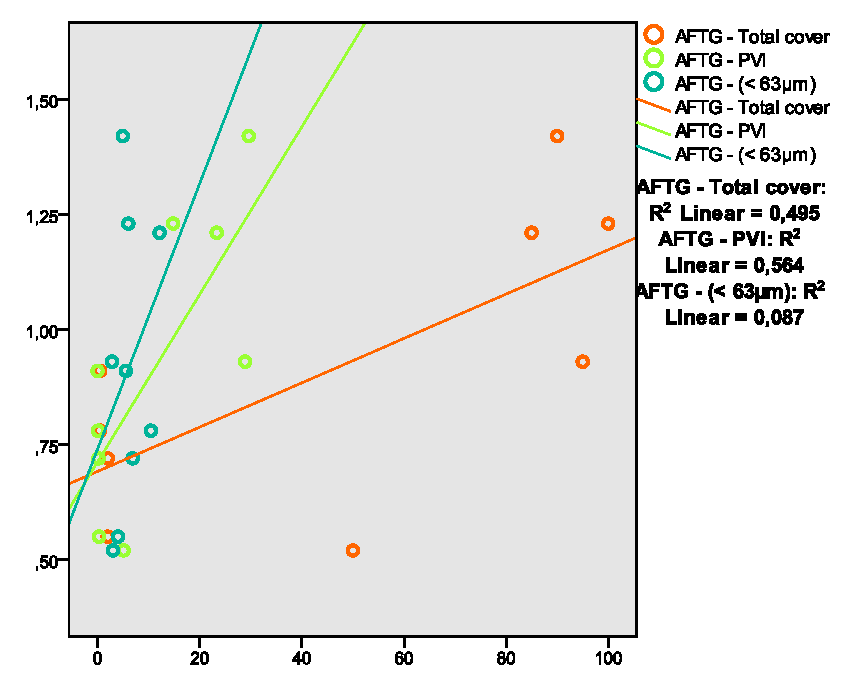
\includegraphics[width=0.75\textwidth]{images/salzsedimentauswertung/afdg1.eps}
\caption[Zusammenhang zwischen organischem Gehalt,\unit{<63}{\mu\metre}-Korngrößenfraktion und Vegetation]{Zusammenhang zwischen organischem Gehalt,\unit{<63}{\mu\metre}-Korngrößenfraktion und Vegetation (Deckung und PVI) an Stationen des Salzgradienten; GB = Geltinger Bucht, OB = Orther Bucht; SH = Salzhaff; V = Vitter Bodden (5.7.2013), G = Griebener Bucht (30.7.2013), SW = Spandowerhagener Wiek}
\label{fig:sg:afdg_regressionen}
\end{figure}

\begin{figure}[!htb]
\centering
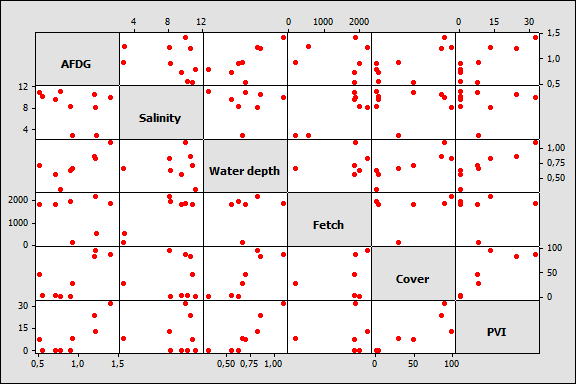
\includegraphics[width=0.75\textwidth]{images/matrixplot/afdg_matrixplot.png}
\caption[Korrelationsmatrix: Organischer Gehalt der Sedimente und 5 Prädikatoren]{Korrelationsmatrix: Median der Korngröße und 5 Prädikatoren ( Salinität, Wassertiefe, Fetch, Bedeckung mit Phytobenths und PVI)}
\label{fig:sg:afdg_matrixplot}
\end{figure}



\begin{table}[!htb]
\centering
\caption[Spearman Rang-Korrelationen zum organischen Gehalt der Sedimente]{Spearman Rang-Korrelationen zum organischen Gehalt der Sedimente (AFDG) entlang des Salzgradienten; 5 Prädikatoren: Salinität, Wassertiefe, Fetch, Bedeckung mit Phytobenthos, PVI}
\begin{tabular}{lrrrrr}

\toprule
& \multicolumn{5}{c}{Correlation / \textit{p}-Value} \\
\midrule
& \multicolumn{1}{c}{AFDG}  & \multicolumn{1}{c}{Salinity} & \multicolumn{1}{c}{Water Depth} & \multicolumn{1}{c}{Fetch} & \multicolumn{1}{c}{Cover} \\

\midrule

Salinity        &       -0,491\\
                &       0,150\\
\midrule
Water depth	    &     	0,669  			&-0,075\\
        		&		0,070   		&0,860\\
\midrule
Fetch  	        &   	0,118   		&0,315			   &0,371\\
        		&		0,801  			&0,491   			&0,468 \\
\midrule
Cover  	        &     	0,596  			&-0,188   			&0,888   		&0,282\\
        		&		0,090   		&0,628   			&0,003   		&0,589\\
\midrule
PVI	            &     	0,669  			&-0,124   			&0,915   		&0,022  	& 0,924\\
        		&		0,049   		&0,750   			&0,001   		&0,968   	&0,000\\
\bottomrule

\end{tabular}
\label{tab:spearman_rank_correlations_afdg}
\end{table}




\begin{table}[!htb]
\centering
\caption[Schrittweise Regression: Organischer Gehalt der Sedimente im Vergleich zu 4 Prädikatoren]{Schrittweise Regression (Rückwärts-Selektion, Alpha für Abnahme: 0,1, N = 4-10): Median der Korngröße im Vergleich zu Salinität, Wassertiefe, Fetch und Bedeckung mit Phytobenthos, das PVI  wurde aufgrund der Korrelation zum PVI und zur Wassertiefe aus dem Modell entfernt}
\begin{tabular}{lrrr}
\toprule
Step      	&     1  &    2     & 		3\\
Constant   	& 2,895  &	3,519  	&	3,231\\
\midrule
Salinity         & -0,81  &	-0,78  	&	-0,74\\
T-Value     & -1,93  &	-2,39  	&	-2,55\\
P-Value     & 0,305  &	0,139  	&	0,084\\
\midrule
Water depth       & 1,56   &	1,67   	&	1,23\\
T-Value     & 1,55   &	2,17   	&	3,34\\
P-Value     &0,364  &	0,162  	&	0,044\\
\midrule
Fetch       &   0,27\\
T-Value    &  0,49\\
P-Value    & 0,711\\
\midrule
Cover      &   -0,38  &	-0,40\\
T-Value   &  -0,51  &	-0,68\\
P-Value   &  0,700  &	0,568\\
\midrule
\midrule
S        &    2,44   &	1,92   	&	1,74\\
$R^2$      &  88,85  &	86,20  	&	83,04\\
$R^2$(adjusted) &  44,26  &	65,50  	&	71,73\\
Mallows Cp  &  5,0  &  	3,2    	&	1,5 \\
\bottomrule
\end{tabular}
\label{tab:spearman_rank_correlations}
\end{table}








   

\clearpage

\section{Diskussion}
\subsection{Zusammenhänge zwischen Vegetation und Sediment in den Hiddenseer Boddengewässern}

Die Vegetation auf den Untersuchungsflächen in der Griebener Bucht und im Vitter Bodden repräsentiert gut die für die Hiddenseer Boddengewässer typischen Artenzusammensetzungen, verglichen mit Beobachtungen von \cite{flugge_2004}, \cite{kunzenbach_1955} und \cite{muller-stoll_1961}.
\\
Im Vitter Bodden, in etwa \unit{80}{\centi\metre} Wassertiefe fanden sich dichte, lose auf dem Boden aufliegende Matten des Blasentanges \textit{Fucus vesiculosus} welcher in dieser Wassertiefe zwischen der Fährinsel und dem Hafen in Vitte das Vegetationsbild prägt und zusammen mit Begleitarten wie \textit{Furcellria fastigiata} \textit{Potamogeton pectinatus}, \textit{Myriophyllum spicatum} und \textit{Chorda filum} vorkommt. Bei \unit{100}{\%}. Das Laichkraut und das Tausendblatt sind sehr häufige und typische Vertreter der Bodden, sie konnte ihr Vorkommen in der Griebener Bucht und im Vitter Bodden ab etwa \unit{50}{\centi\metre} Wassertiefe oft beobachtet werden. Für \textit{Myriophyllum spicatum}, nicht jedoch für \textit{Potamogeton pectinatus} fand \cite{flugge_2004} in der Griebener Bucht eine positive Korrelation mit der Wassertiefe. 
\cite{muller-stoll_1961}  beschreibt \textit{Potamogeton pectinatus} als dominante bestandsbildende Art in \unit{1,5 bis 4}{\metre} Wassertiefe und grenzt dies als Zone zu Beständen aus \textit{Chara baltica} und \textit{Fucus vesiculosus f. filiformis} ab. Die zuletzt genannten Arten kommen nach  \cite{muller-stoll_1961} in einer Wassertiefe von \unit{0,5 bis 2,5}{\metre} vor. 

Obwohl das Phytobenthos des vegetationsdominierten Standortes in Vitte nur einen Anteil von \unit{8-17}{\%} an der Wassersäule hat, ist die Biomasse auf den Flächen mit im Mittel \unit{890}{\gram\per\metre\suqared} (Trockensubstanz) im August extrem hoch. Auf gleich großen Ernteflächen im Golf von Riga fand \cite{martin_1999} ebenfalls sehr hohe Biomassewerte in festsitzenden \textit{Fucus vesiculosus} -Beständen. Zwischen Ainazhi und Kabli in \unit{1,5}{\metre} Tiefe fand er die höchsten Biomassewerte im Golf von Riga von \unit{2700}{\gram\per\metre\suqared} (Feuchtgewicht). Grund für die hohen Biomassewerte könnten die Derbheit der Thalli und das große Masse-Volumen-Verhältnis sein, denn die Individuen waren annähernd kugelförmig mit einer in sich hohen Dichte. Die Flächen waren zudem zu \unit{100}{\%} bedeckt und die Braunalgen zu solch dichten Matten zusammengeschoben, dass  der Wasseraustausch zwischen den Wasserschichten innerhalb des Algenbettes und darüber erschwert war, sodass sich nach eigenen Beobachtungen von Mai bis Anfang Juni eine deutliche Thermokline feststellen ließ (in gleicher Wassertiefe ohne dichte \textit{Fucus vesiculosus f. balticus} -Bestände wurde diese Thermokline nicht festgestellt). 

Sowohl die Biomasse als auch das PVI veränderten sich in der Untersuchungsgruppe. Von Juni bis August stieg der Anteil der Pflanzen in der Wassersäule um \unit{7,3}{\%} und auch in den 2 Biomassekartierungen im Juni und im August wurde ein mittlerer Biomassezuwachs von \unit{90}{\gram\per\metre\squared} (Trockengewicht) festgestellt. 
In dem von Feinsand und Mittelsand geprägten Sediment konnte jedoch keine Veränderung der mittleren Korngröße festgestellt werden. Ebenso änderte sich der Anteil der \unit{<63}{$\mu$\metre} Fraktion und der organische Gehalt nicht im Jahresverlauf. 
\\
Die spärlich besiedelte Vergleichsgruppe des Vitter Standortes befand sich etwa \unit{300}{\metre} weiter östlich auf einer Sandbank, das Wasser war hier mit einer mittleren Tiefe von \unit{62}{\centi\metre} etwa \unit{20}{\centi\metre} flacher. An einigen Untersuchungstagen mit Wasserständen unter dem Mittel wurden hier teilweise nur \unit{30-40}{\centi\metre} Tiefe gemessen. Erst ab Juli befanden sich hier lichte Characeen-Bestände von \textit{Chara canescens} und \textit{Chara baltica}, typische Brackwassercharaceen, die auch stark schwankende Salzgehalte vertragen \citep{blindow_2003, blumel_2003}. 

\textit{Chara canescens} kommt hauptsächlich in Flachwasserbereichen unter \unit{50}{\centi\metre}  bis maximal \unit{1}{\metre} Wassertiefeiefe \citep{blindow_2003} vor und überwintert hauptsächlich in Form von Oosporen \cite{wahlstedt_1862}. Auch \textit{Chara baltica} ist typisch für Flachwasserbeiche, sowohl in geschützten Buchten als auch an exponierten Ufern \citep{blumel_2003}. Die Art überwintert hauptsächlich in Form von Bulbillen, selten als Pflanze oder in Form von Oosporen \cite{blumel_2003}. Während \cite{flugge_2004} beide Characeenarten  bereits Ende Mai kartieren konnte, waren sie im Untersuchungsjahr 2013 erst ab Juni in den Hiddenseer Bodden zu beobachten. Daraus lässt sich schließen, dass sich die Characeen-Vegetation aufgrund des lang anhaltenden Winters allgemein erst recht spät im Jahr entwickelt hat.
Neben den Characeen fanden sich ab August auch \textit{Ruppia cirrhosa}, \textit{Potamogeton pectinatus} und \textit{Myriophyllum spicatum} auf den Flächen im spärlich besiedelten Bereich des Vitter Boddens. Die Tatsache, dass sie erst so spät im Jahr kartiert wurden, lässt darauf schließen, dass sie im Gegensatz zu den Pflanzen im dicht besiedelten Bereich aus Samen ausgekeimt sind und nicht als Sporophyt überwintert haben.

Wähhrend sich die Bedeckung und das PVI an dieser Untersuchungsgruppe von unit{0}{\%} auf \unit{5 bzw. 0,6}{\%} erhöht haben, ändert sich die Korngrößenverteilung, der Median der Korngröße der mittel- und feinsanddominierten Sedimente nicht im Verlauf der Wachstumssaison.

Im Vergleich beider Untersuchungsgruppen in Vitte wurde festgestellt, dass das Sediment in der östlich gelegenen vegetationsarmen Gruppe im Mittel etwas gröber ist, der Anteil des organischen Gehaltes jedoch identisch. 

Sowohl für die Griebener Untersuchungsgebiete als auch für die Vitter Untersuchungsgebiete kann gesagt werden, dass sich die Vegetationsstruktur (mittlere Wuchshöhen und PVI) im Jahresverlauf ändern und dass es einen Wechsel an Dominanzen verschiedener Arten im Verlauf der Wachstumssaison gibt. Die Sedimentstruktur jedoch ändern sich nicht im Verlauf der Wachstumsperiode. Dies hängt damit zusammen, dass andere Faktoren wie Wassertiefe und Fetch neben weiteren nicht in Betracht bezogenen Faktoren einen Einfluss auf die Korngrößenverteilung haben können. 



\subsection{Diskussion der Ergebnisse für für die Stationen entlang des Salzgradienten}

Zum Zeitpunkt der Untersuchungen entlang des Salzgradienten Ende Juni/ Anfang Juli gab es an allen 6 Stationen überall einen deutlichen Unterschied in der Bedeckung mit Makrophytobenthos und in deren Anteil an der Wassersäule zwischen den Untersuchungsgruppen. Ausgenommen hiervon ist die Spandowerhagener Wiek, an der kein vegetationsarmer Standort vorgefunden werden konnte. Die Deckung betrug an allen spärlich besiedelten Stellen maximal \unit{2,5}{\%} und das PVI maximal \unit{0,3}{\%}. Aufgrund der sehr verschiedenen PVI- Werte und Deckungsgrade der dicht besiedelten Standorte war es interressant mithilfe von nichtparametrischen Regressionsanalysen zu untersuchen, ob und in welchem Maß die genannten Vegetationsparameter die mittlere Korngröße beeinflussen. Da das Verhältnis von Bedeckungsgrad und PVI stark schwankt (in Vitte ist es beispielsweise wesentlich größer als in der Orther Bucht), wurde der Einfluss beider Vegetationsparameter auf das Sediment getrennt voneinander betrachtet. 

Es zeigt sich, dass es keinen Zusammenhang gibt, sowohl zwischen dem PVI und dem Median der Korngröße als auch zwischen der Bedeckung mit Phytobenthos und dem Median der Korngröße. Ebenso konnte kein Zusammenhang zwischen den Vegetations-Strukturparametern und dem Siltanteil der Sedimente gefunden werden.

Die Tatsache, dass sich neben der Vegetationsstruktur und Artenzusammensetzung die Standorte weiterhin in vielen anderen Aspekten voneinander unterscheiden macht es schwierig, allgemeingültige Schlüsse aus diesen Regressionsanalysen zu ziehen und auf den Zusammenhang bzw. auf eine Unabhängigkeit zwischen der Makrophytobenthosstruktur und dem Sediment zu schließen. Die Stationen unterscheiden sich nämlich auch in ihrer Wassertiefe voneinander. Diese wiederum hat einen direkten Einfluss auf die Fließgeschwindigkeit am Grund und damit auf die Bodenschubspannung. Aufgrund der unterschiedlichen geografischen Lage ist auch der Fetch aus der allgemeinen Hauptwindrichtung sowie der aktuelle Fetch während des Untersuchungszeitpunktes sehr unterschiedlich. Der Fetch ist nach \cite{laenen_1996} jedoch ein Parameter, der ebenfalls in die Berechnung der Bodenschubspannung eingeht, demzufolge müsste eine zusätzliche Abhängigkeit der Korngröße vom Fetch bestehen. Außerdem unterscheidet sich der Salzgehalt der Stationen voneinander, welcher wiederum nach \cite{schwenke_1995}  den Wuchs der Algen beeinträchtigt und für eine Veränderung der Artengemeinschaften im Ökosystem führt, da der Salzgehalt und seine Schwankungen eine von Organismen nur in bestimmten Toleranzbereichen ertragen wird. So könnte der Salzgehalt beispielsweise auch einen Einfluss auf die Benthosfauna haben.

In der schrittweise durchgeführten Regression unter Einbeziehung der Parameter Salinität, Wassertiefe, Fetch und PVI zeigt sich, dass eine Abhängigkeit der mittleren Korngröße von der den Faktoren Fetch und Salinität in Kombination die höchste Wahrscheinlichkeit aufweist. Es ist jedoch möglich, dass andere, unbekannte Faktoren wie zum Beispiel anthropogene lokale Einflüsse eine Rolle spielen.

Betrachtet man die Standorte und deren Untersuchungsgruppen separat voneinander, so lässt sich feststellen, dass  an 4 von 5 Stationen das Sediment in der dicht besiedelten Untersuchungsgruppe im Mittel feiner war, nämlich an den zwei Hiddenseer Standorten, im Salzhaff und in der Griebener Bucht. In der Geltinger Bucht war das Sediment in der spärlich besiedelten Untersuchungsgruppe etwas feiner. Aufgrund der geringern Stichprobengröße (n=1) für die Sedimentanalyse (die Hiddenseer Standorte werden hiervon ausgeschlossen) lässt sich nicht mit Sicherheit sagen, ob es sich in jedem Fall um einen signifikanten Unterschied handelt, jedoch stellt sich die Tendenz heraus, dass in Makrophytenbeständen das Sediment feiner ist. Nach \cite{lindner_1978} kann es jedoch auch sein, dass nicht der Makrophytenbestand die Korngröße beeinflusst, sondern dass die Pflanzen feine Korngrößen bevorzugen, weil sie hier optimale Strukturen und Nährstoffgehalte vorfinden.

Aus den Analyseergebnissen lässt sich also unter Vorbehalt schließen, dass die erste Hypothese dieser Arbeit zutrifft. Die Hypothese, dass der Anteil der Makrophyten an der Wassersäule negativ bzw. überhaupt mit der mittleren Korngröße korreliert, muss jedoch abgelehnt werden.

Bei Betrachtung des Siltanteils wurde ein ähnliches Ergebnis gefunden. Während es keine Korrelation zwischen den Parametern der Vegetationsstruktur und dem Siltanteil der Sedimente gibt, zeichnet sich ebenfalls eine leichte Tendenz zwischen dicht und spärlich besiedelten Standorten heraus: In der Gribener Bucht und dem Vitter Bodden wurde im dicht besiedelten Bereich ein signifikant höherer Anteil der Siltfraktion festgestellt als im spärlich besiedelten Bereich, das gleiche, jedoch nicht statistisch abgesichert, gilt auch für das Salzhaff. In der Geltinger Bucht und der Orther Bucht wurden umgekehrte Verhältnisse festgestellt. 

Auch der Anteil zwischen der Vegetationsstruktur und dem Organischen Gehalt des Sedimentes wurden untersucht. Nach \cite{steinhardt_2001} verringert ein großer Anteil der organischen Substanz die mittlere Korngröße, da sie aus kleinen Partikeln besteht. Deren Einfluss auf die gemessene mittlere Korngröße kann jedoch verfälscht sein, da die organischen Partikel häufig zu Aggregaten verbunden sind und diese mit dem Nassiebe-Verfahren nicht in ihre Bestandteile zerlegt wurden. Mittels Veraschung der Proben konnte festgestellt werden, dass der organische Gehalt, mit Ausnahme dem in der Orther Bucht, an den makrophytendominierten Standorten stets erhöht war. Eine mäßige Erhöhung um \unit{32 bis 43}{\%} des Trockengewichtes wurden in den Sedimentes des Vitter Boddens und des Salzhaffes gefunden. Dies waren Seegras- und Blasentang-dominierte Standorte mit extrem hohen Deckungsgraden von  \unit{80 bis 90 bzw. 100}{\%} ,im Salzhaff war ebenfalls der Anteil der Makrophyten an der Wassersäule mit\unit{20-30}{\%} sehr hoch. Der Unterschied des organischen Gehaltes in der Orther Bucht war mit \unit{3}{\%}  Trockensubstanz nur sehr gering. Grund dafür, dass der Gehalt nicht erhöht war, könnte sein, dass der Großteil der allgemein nicht sehr dichten Vegetation (es wurden Deckungsgrade von durchschnittlich \unit{50}{\%} und PVI-Werte von \unit{5}{\%} vorgefunden) zum großen Teil durch Matten freischwimmender, filamentöser Algen verursacht wurde, die vermutlich ebenso wie die filamentösen Algen bei Hiddensee nicht so weit in die Wachstumssaison hinein überdauern. In Grieben war der organische Anteil bei der vegetationsreichen Untersuchungsgruppe mit einer Differenz von \unit{276}{\%} Trockengewicht extrem erhöht. Diese hohen Werte sind vermutlich anthropogen oder durch die Abtrabung humusreichen Oberbodens verursacht, denn die Untersuchungsgruppen in Grieben lagen auf unterschiedlichen Seiten der Bucht und der vegetationsdominierte Bereich nahe des Ortes Grieben. Dahinter schließen sich durchlässige sandige Böden und die Dornbusch-Erhebung an. Auch könnte es sein, dass aufgrund der Dorfnähe in früheren Zeiten Abwässer in die Griebener Bucht eingeleitet wurden. 

In den Regressionsanalysen zeigt sich nur ein mäßiger Zusammenhang zwischen dem organischen Gehalt des Sedimentes und der Deckung sowie zwischen Organik und PVI. Auch die These bezüglich des Zusammenhangs zwischen Feinpartikelanteil (Silte) und organischem Gehalt der Sedimente  von \cite{steinhardt_2001} bestätigt sich nicht, was jedoch an den bereits erwähnten Problemen der Nassiebung liegen könnte. 

Im schrittweise durchgeführten Regressionsmodell unter Berücksichtigung der Parameter Salinität, Wassertiefe, Fetch und Bedeckung durch Makrophyten wurde festgestellt, dass die alleinige Berücksichtigung der Parameter Salinität und Wassertiefe die organischen Gehalte der Sedimente am besten erklären. Dies deckt sich mit den Untersuchungsergebnissen von \cite{steinhardt_2001}, der ebenfalls keinen Zusammenhang zwischen der Makrophytenbedeckung und der mittleren Korngröße im Salzhaff gefunden hat, jodoch eine starke Abhängigkeit der mittleren Korngröße und des organischen Gehalts mit der Wassertiefe. Nach eigenen Ergebnissen korreliert die mittlere Wassertiefe positiv und die Salinität negativ mit dem organischen Gehalt. Das gleiche Ergebnis für den organischen Gehalt erhielt auch  \cite{steinhardt_2001}.





\clearpage

\section{Zusammenfassung}
Die Stationen entlang des Salzgradienten ....

\clearpage

%%%%%%%%%%%%%%%%%%%%%%%%%%%%%%%%%%%%%%%%%%%%%%%%
% Ende des Textkörpers
%%%%%%%%%%%%%%%%%%%%%%%%%%%%%%%%%%%%%%%%%%%%%%%%


%%% Literatur-Verzeichnis 

% damit wird die Datei literature.bib aus dem gleichen Verzeichnis benutzt. Zum Bearbeiten der Datei empfehle ich pybliographer oder Zotero!
\bibliography{literature_30th_march_mendeley.bib}

% hier einen passenden Stil für die Darstellung der Zitate im Text und im Lit.-Verz. angeben!
\bibliographystyle{munich} 

\newpage

%%% Anhang %%%%%%%%%%%%%%%%%%%%%%%%%%%%%%%%%%%%%

\pagestyle{plain} 

\section*{Anhang} % Kapitel ohne Nummerierung
\addcontentsline{toc}{section}{Anhang}

\begin{appendix}

% Hier können jetzt nach belieben Bilder, Tabellen, Karten und sogar ganze PDF-Dokumente eingebunden werden! Z.B.:


%\begin{figure}[htb]
%\centering
%\includegraphics[width=\textwidth]{images/map.png}
%\caption{Bildunterschrift}
%\label{fig:map.png}
%\end{figure}


% EInbindung PDF Seiten according to : http://gb01.blogspot.de/2008/03/include-pdf-in-latex.html
% Globals: include all pages, don't auto scale
%\includepdfset{pages=-}

% Include the PDF files, scaling as required
%% \includepdf[scale=1.25]{title.pdf}
%\includepdf[landscape, fitpaper]{images/map.pdf}



\end{appendix}
%%%%%%%%%%%%%%%%%%%%%%%%%%%%%%%%%%%%%%%%%%%%%%%%%
\end{document}
